\section{Introduction}

Sections of this chapter appear in a manuscript submitted to Springer link as part of the International Conference on Computational 
Science (ICCS) 2025 in the Computing and Data Science for Materials Discovery and Design track, submission number 259 and is
% [author and/or editor(s) of contribution], [volume and/or contribution title], [year of publication], [publisher (as it appears on our copyright page)] \
reproduced with permission of Palgrave Springer Nature. 

Emulsions can adopt a variety of microstructures depending on fluid volume fractions and the affinity of stabilizing agents for each phase. Among these, bicontinuous 
interfacially jammed emulsion gels (bijels) are characterized by a tortuous, co-continuous network of immiscible fluid domains stabilized by colloidal particles. This 
unique architecture lends itself to numerous advanced applications, including membrane fabrication, catalyst supports, battery electrodes, and pharmaceutical delivery 
systems. Bijels form through the arrest of spinodal decomposition in partially miscible fluid mixtures: as phase separation proceeds, the interface sweeps through the 
system, adsorbing particles until the interfacial area becomes saturated, resulting in jamming. Microstructural features such as domain size, continuity, and interfacial 
curvature critically influence material performance, affecting properties like mass transport, mechanical stability, and surface reactivity. Since their discovery via 
simulation and subsequent experimental realization, research on bijels has expanded significantly, exploring diverse synthesis conditions and scalable processing methods.

The functional properties of bijels are inherently linked to their internal structure. For instance, lower tortuosities in the direction of ion transport yield improved 
charge rates and cycling stability in battery electrodes \cite{ebner_tortuosity_2014, samdani_bicontinuous_2017}. In liquid-liquid extraction, the characteristic pore 
lengthscale determines molecular selectivity \cite{khan_nanostructured_2022}, while in pharmaceutical applications, domain size influences drug release rates and cellular 
behavior \cite{vanoli_bijels_2022, thorson_bijel-templated_2019}. Given the sensitivity of these properties to microstructural characteristics, the ability to dynamically 
modify the morphology of bijels presents a promising strategy to adapt their behavior in situ for targeted performance.

Stimuli-responsive emulsions have garnered increasing interest for applications requiring dynamic control over material properties, including enhanced oil recovery, reaction 
separation, and therapeutic delivery \cite{tham_magnetophoresis_2021, cui_stabilizing_2013, rozynek_opening_2019, lu_controllable_2020}. These systems operate by using 
external stimuli to alter interfacial configurations, enabling modulation of permeability, interfacial area, and morphology. For example, in emulsions stabilized by 
spherical particles, electric fields can induce droplet deformation via particle unjamming and migration before re-establishing interfacial jamming \cite{cui_stabilizing_2013}. 
Among various external stimuli, magnetic fields are particularly attractive due to their remote addressability, material compatibility, and bio-relevance. 
Core-shell ferrite-hydroxyapatite nanorods, for instance, exhibit reversible morphological changes depending on initial particle orientation and field direction 
\cite{nakayama_stimuli-responsive_2018}. In magnetically stabilized Pickering emulsions, magnetophoresis has been shown to drive particle migration and interfacial 
distortion or collapse \cite{tham_magnetophoresis_2021, yang_rapid_2020, misra_magnetic_2020}. Notably, Karthikeyan and Schiller demonstrated that magnetic fields applied 
during bijel formation can bias domain coarsening, producing anisotropic microstructures via orientation-specific jamming \cite{karthikeyan_formation_2024}. However, the 
structural response of bijels to magnetic fields after formation remains poorly understood.

This study investigates the post-formation structural response of bijels stabilized by ellipsoidal magnetic particles under the influence of externally applied magnetic fields. 
Using a hybrid Lattice Boltzmann Method coupled with Molecular Dynamics, we simulate the formation and evolution of bijel structures stabilized by rod-like particles modeled as 
magnetic dipoles. We find that increasing the applied magnetic field after formation induces significant microstructural changes, including increased domain anisotropy and 
coarsening, up to a saturation threshold. In contrast, decreasing or removing the magnetic field results in minimal morphological change, suggesting a strong hysteresis effect. 
Analysis reveals that particle unjamming, reorientation at the interface, and subsequent re-jamming are responsible for these structural transformations.

To understand the saturation behavior, we applied magnetic fields of varying strength to bijel templates formed under increasing initial field conditions. We observed that 
a greater initial nematic order parameter negatively correlated with the extent of microstructure change. Finally, switching off the magnetic field in pre-aligned bijels had little 
impact on the microstructure, indicating that the jammed interfacial network prevents reversal of anisotropic features. These findings underscore the importance of processing 
history and demonstrate how magnetic field manipulation, in combination with anisotropic particle stabilization, enables tunable, on-demand microstructure control in bijels, 
offering new capabilities for adaptive material design.

\section{Results}\label{sec:results_p2}
\subsection{Hysteresis curve}\label{section:hysteresis_curve}

Bijels have proposed applications as soft matter based material templates, drug delivery vectors and separations systems. The materials 
performance in each application is dependent upon the microstructure of the bijel template. Many of the applications listed above benefit 
from stimuli response, allowing for in-situ microstructure tuning to offer reversible modifications of material permeability. In this section, we analyze
whether stimuli responsive bijels provide access to reversible structural modifications.

We begin our investigation by characterizing the microstructure changes observed on bijels stabilized with prolate ellipsoids with a 
particle volume fraction of $\phi_p = 0.1$. We only focus on one system here as the mechanism for stimuli response shown in Aim 1 is identical
for both systems. Therefore We expect that the qualitative trends between prolate and oblate particles will be matched. We select prolate particles
as they are more readily synthesizable in experiments. 

We apply a constant magnetic field of $\bar{B}_z = 0.2$ onto bijels that were simulated 
with no magnetic field. Once the microstructure has reached its new state, we ramp up the magnetic field to $\bar{B}_z = 0.5$ and 
finally $\bar{B}_z = 1$. We then apply the opposite procedure to reduce the applied field strength, resulting in a magnetic field 
ramp of $\bar{B}_z: 0 \rightarrow 0.2 \rightarrow 0.5 \rightarrow 1 \rightarrow 0.5 \rightarrow 0.2 \rightarrow 0$. We characterize the 
microstructure changes observed through calculating the domain size, defined as the first moment of the spherically averaged structure factor. 
We calculate the hysteresis 
curve by selecting the domain size at the final timestep of each magnetic field change. We then plot these domain sizes against the magnetic field 
applied to obtain them and split them in the descending and ascending magnetic field directions to demonstrate the differences observed. We plot 
these results in Figure \ref{fig:hysteresis_curve}

\begin{figure} 
    \centering 
    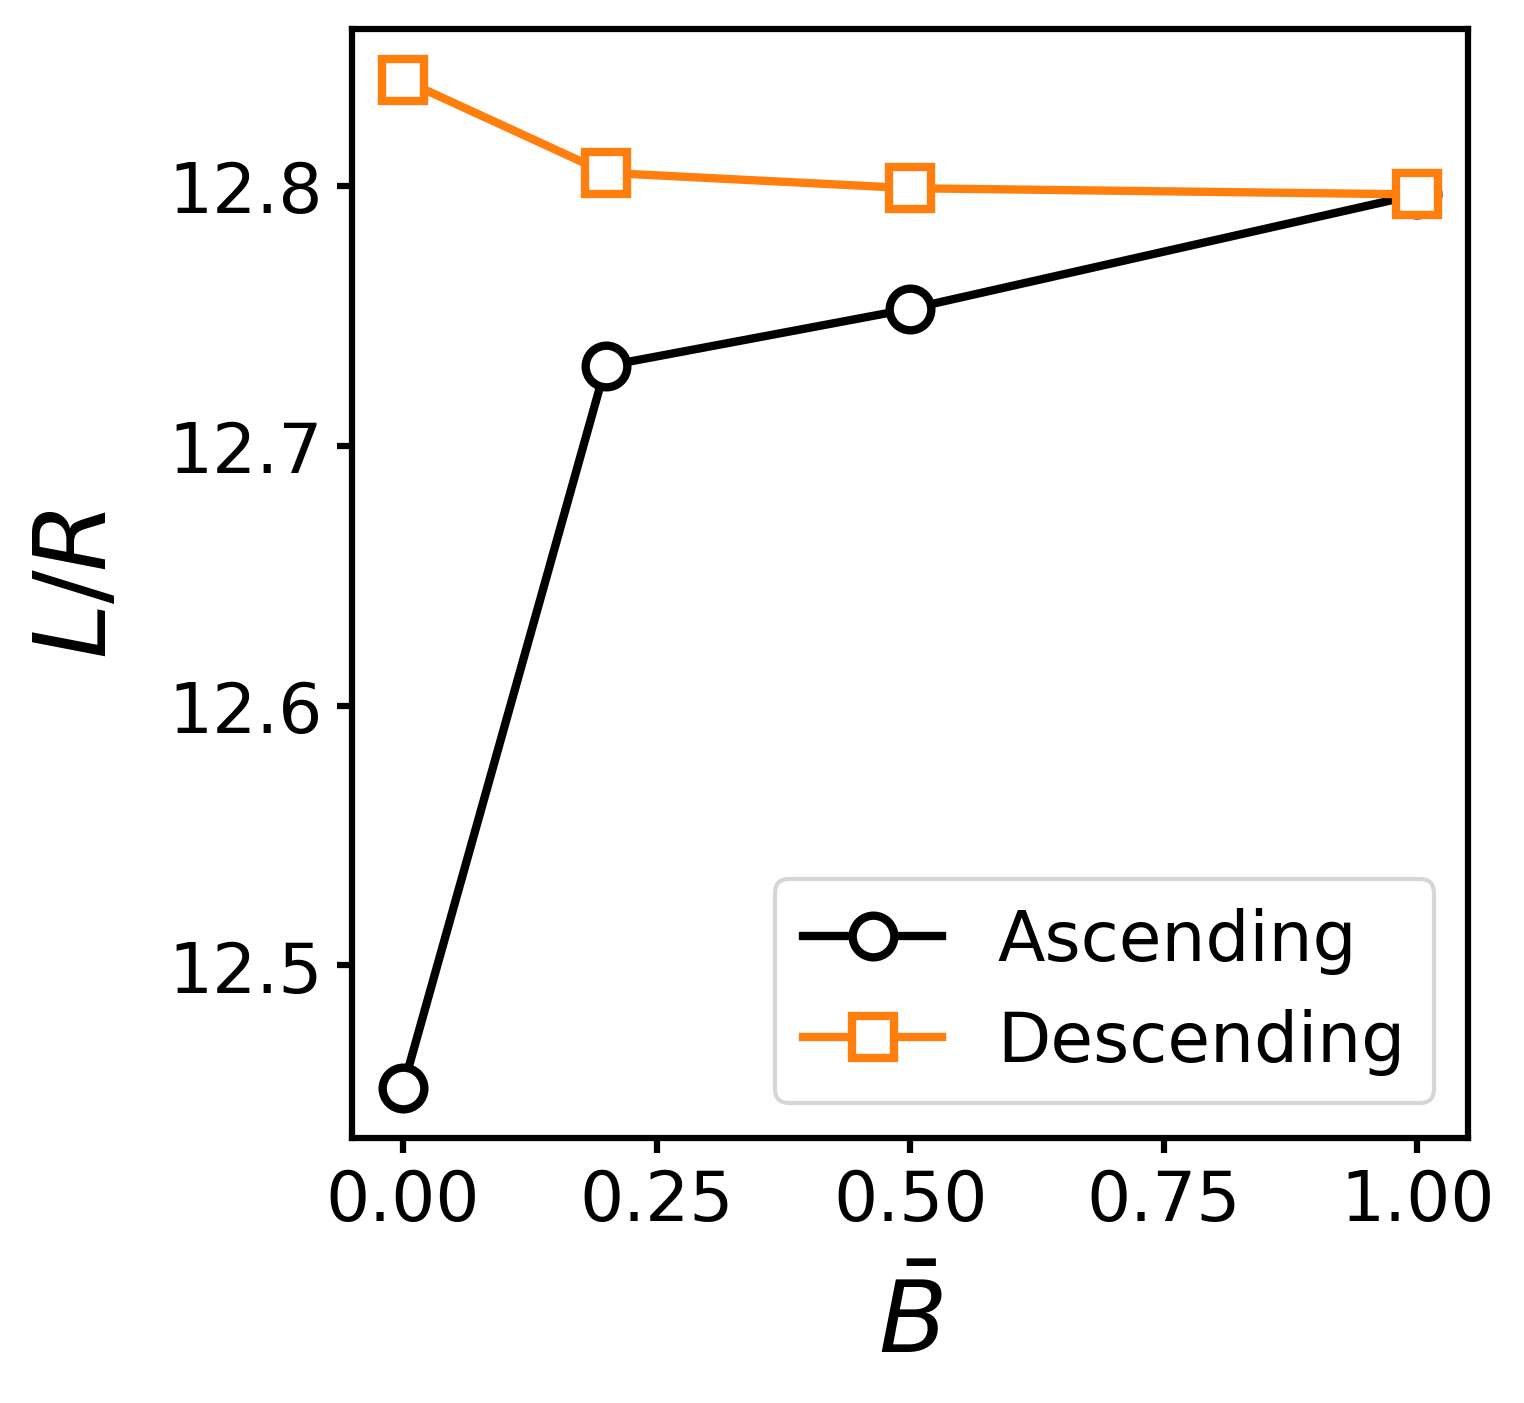
\includegraphics[scale=0.5]{../figures/results/paper2/hysteresis_curve.png} 
    \caption{Plot of the hysteresis curve of a bijel stabilized by magnetically responsive prolate particles. We observe that the domain size increases as we 
    increase the applied magnetic field strength. However, upon decrease of the applied field strength the microstructure does not return to its previous value,
    demonstrating microstructure hysteresis.} 
    \label{fig:hysteresis_curve} 
\end{figure}

Figure \ref{fig:hysteresis_curve} demonstrates the hysteresis response of the bijel microstructure, characterized by a difference in the average domain size
when increasing and decreasing the magnetic field. The increase in the average domain size when applying the magnetic field is due to domain coarsening caused by 
reorientation of particles to the magnetic field strength, reducing the interfacial coverage. When decreasing the magnetic field strength, 
the domain size does not return to the original value meaning that that the microstructure of the bijel is unaffected by 
the reduction and eventual removal of the applied magnetic field. 

This behavior is also observed in past work investigating the shape deformation of particle stabilized emulsions under 
electric fields. \cite{cui_stabilizing_2013} Cui et al. demonstrated that the particles unjammed and rejammed into a new kinetically arrested state resulting in
the droplet being elongated in the direction of the applied field. This suggests that the particles at the interface of magnetically responsive bijels are in
in a kinetically trapped configuration. Cui et al. used spherical particles in their emulsion response experiments while we use ellipsoidal particles. Additionally,
Figure \ref{fig:hysteresis_curve} shows that the response of the bijel is dependent upon the field strength applied.
In the following sections, we investigate the impact of magnetic field strength and the initial ordering of the particle monolayer on the observed stimuli response.

\subsection{Field strength dependence on domain size}
\label{section:field-strength-dependence-on-domain-size}

From the results in Figure \ref{fig:hysteresis_curve}, we show that the domain size change is dependent upon the applied magnetic field. As porous materials templates,
the microstructure of the material is of interest as it controls the performance of the material. Additionally, in many of the proposed stimuli responsive applications
for bijels, the timescales of response is important to characterize and would also provide a mechanistic understanding of the reasons why the microstructure changes 
occur. In this section, we analyze the structural response of bijels by assessing the response of bijels stabilized by particles with volume fraction of 
$\phi_p = 0.1$ simulated under no applied field to an applied field in the range $\bar{B} = 0, 0.2, 0.5, 1$. We begin our investigation by visualizing the structure before 
and after the application of magnetic fields.

\begin{figure} 
\centering 
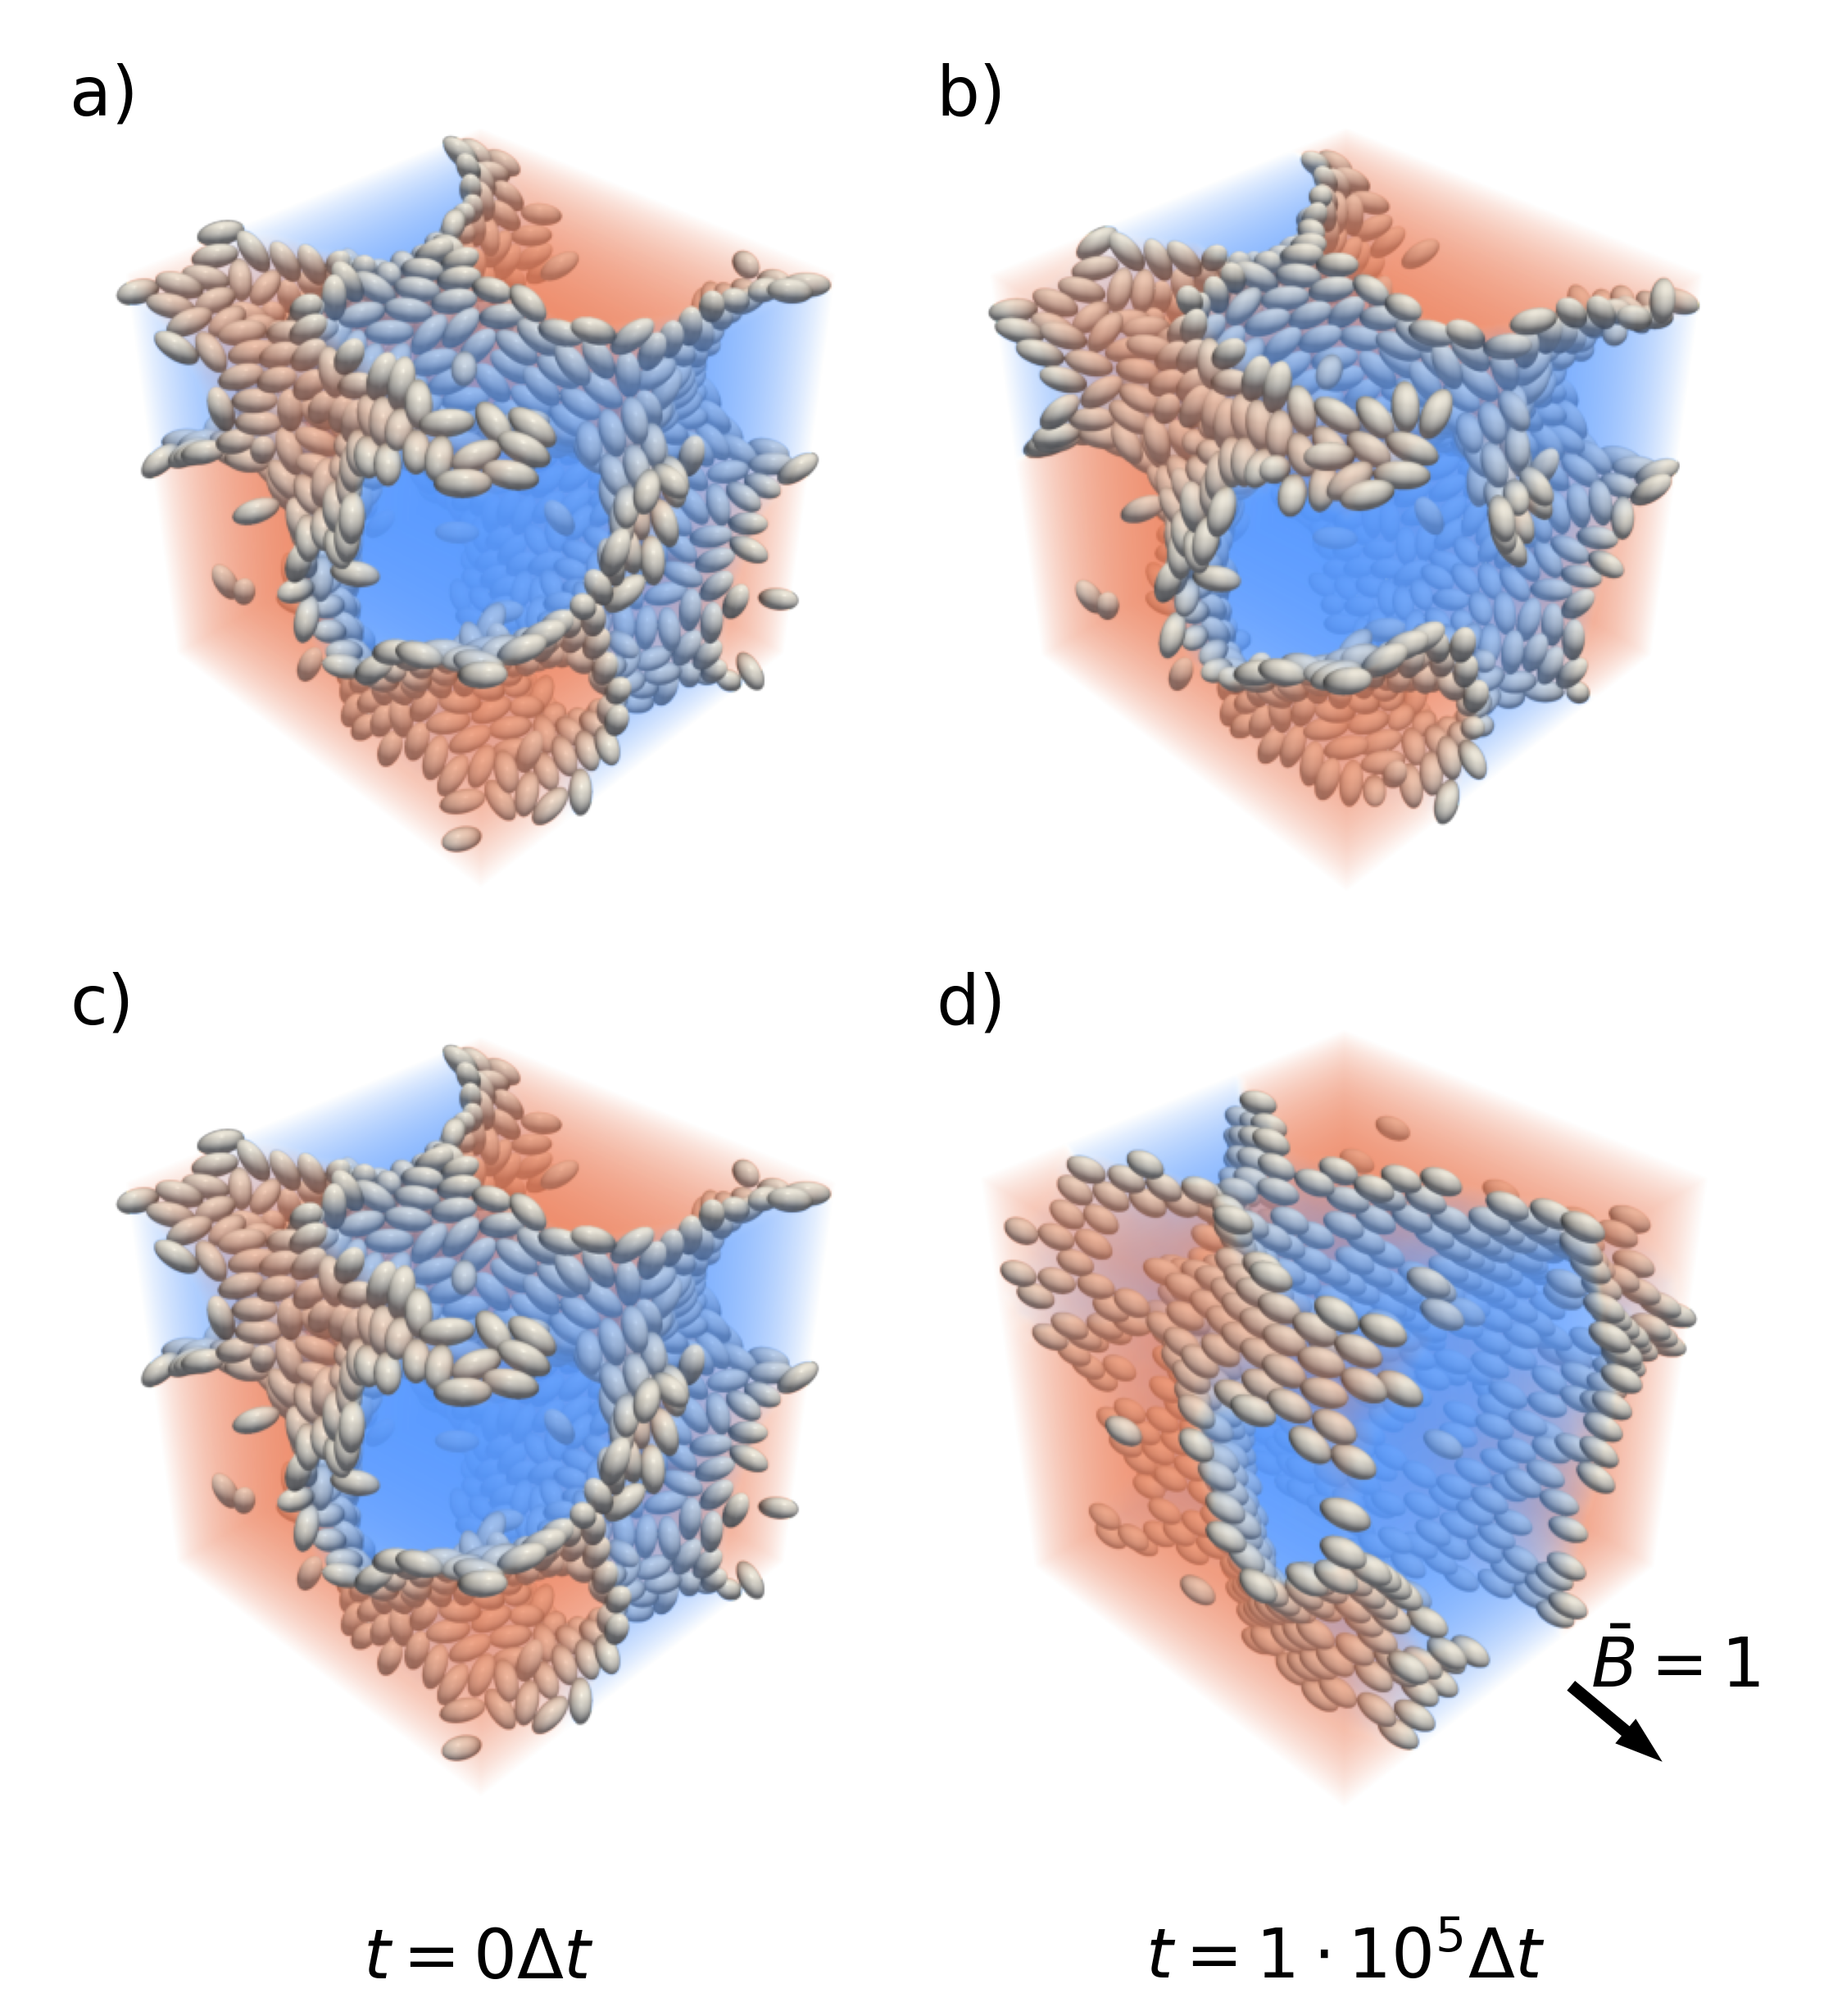
\includegraphics[scale=0.4]{../figures/results/paper2/microstructure_viz-field_on.png} 
\caption{Visualizations of bijels stabilized by oblate and prolate particles simulated under no fields at $t = 0$ (left columns) and $t = 10^5$ (right columns). The first 
         and third row detail the microstructure evolution for oblate and prolate particle stabilized bijels with no applied field while the second and fourth rows show 
         bijels stabilized by oblate and prolate particles respectively with a field strength of $\bar{B} = 1$ applied. Particle reorientation to the direction of the 
         field can be seen upon application of the magnetic field, resulting in microstructure changes driven through domain coarsening until the particles jam. We see 
         similar behavior in bijels stabilized by oblate particles upon application of the magnetic field.}
\label{fig:microstructure_viz-field_on} 
\end{figure}

In Figure \ref{fig:microstructure_viz-field_on} we show representative snapshots of the bijel at the initial and final timestep with $\bar{B}_z = 0$ and $\bar{B}_z = 1$. 
Upon application of the field, particles align to the direction of the field. As the particles orient to the field, they disrupt the packing of particles at
the interface. This causes domain coarsening as the particles rearrange into new positions before rejamming in place once the interfacial
area and particle cross sectional area match. Domain coarsening observed in the figure can be explained through the ordering of particles at the interface, causing a 
reduction in the available area that the particles have for stabilization. To characterize the length scale of the microstructure upon application of the magnetic field,
we calculate the domain size. To correlate the microstructure evolution to the ordering of the particle monolayer to the magnetic field, we overlay the time evolution of the
nematic order parameter on the domain size. \cite{veerman_phase_1992} 

\begin{figure} 
\centering 
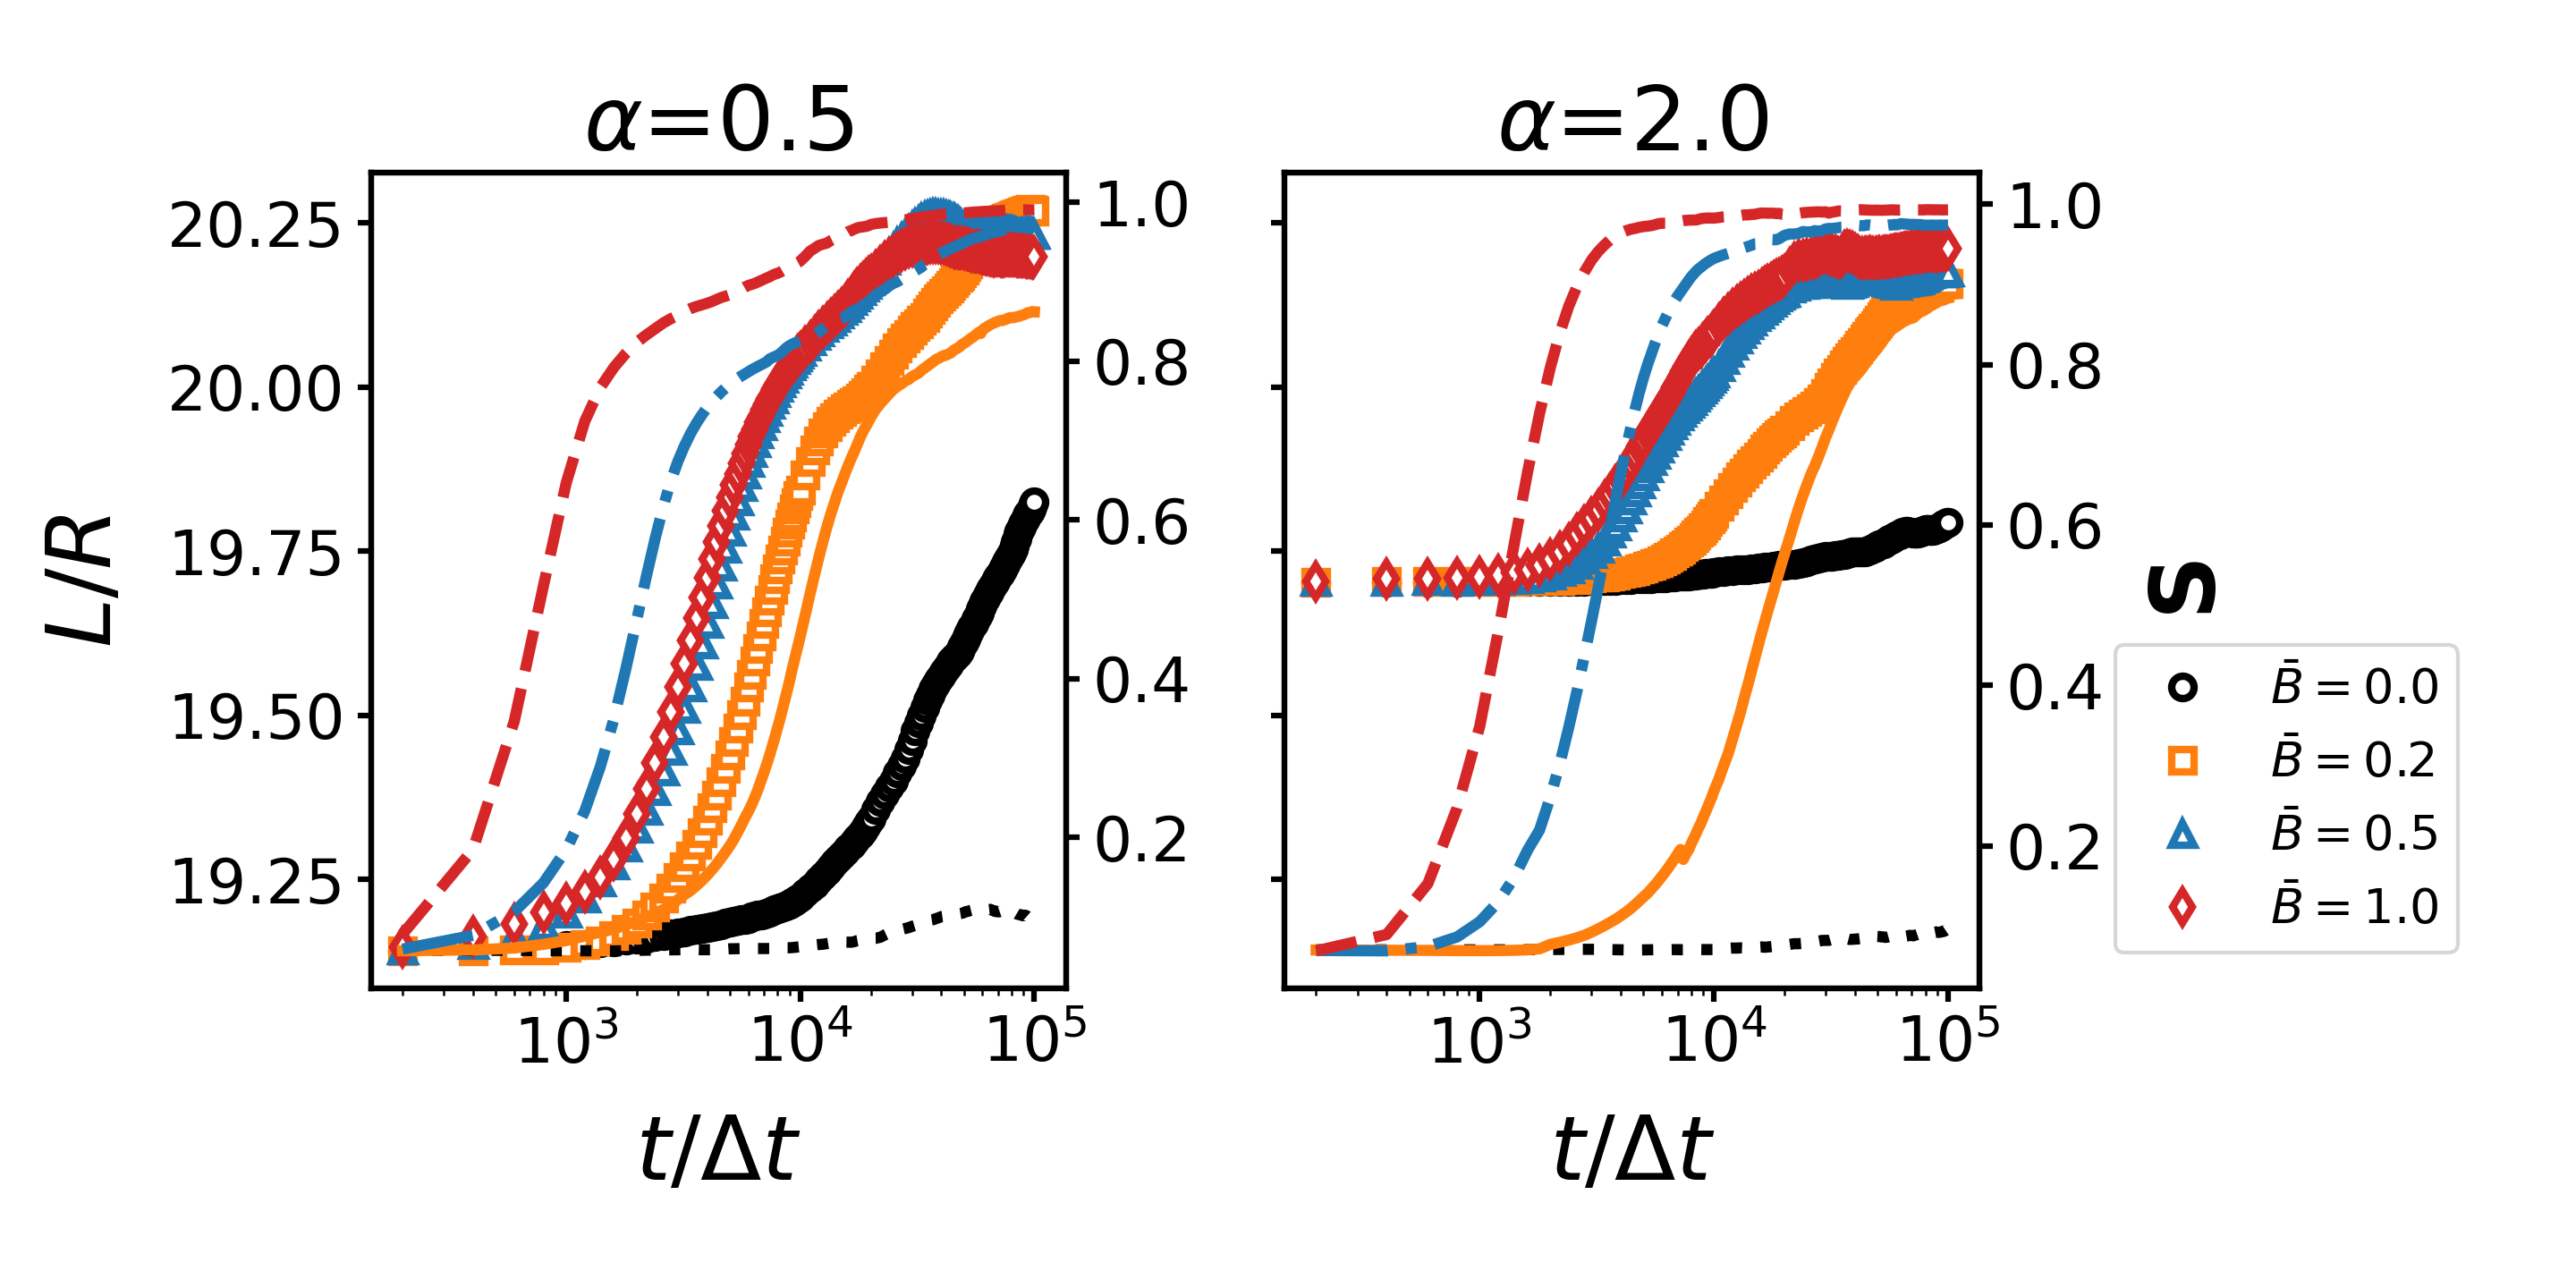
\includegraphics[scale=0.5]{../figures/results/paper2/domain_size-field_on.png} 
\caption{Plotting the spherically averaged domain size normalized with $R_p$($L/R$) of the particle at different magnetic field strengths, $\bar{B}$, and the nematic order 
         parameter $S$ in lines. We quantify the domain size and ordering of the particles, and show that the change in both parameters are correlated with the strength of 
         the applied magnetic field.} 
\label{fig:domain_size-field_on} 
\end{figure}

We normalized the domain size results by the volume equivalent sphere radius, $R = 7.9$ in Figure \ref{fig:domain_size-field_on} The results indicate that upon 
applying a magnetic field to a bijel initially formed without one, the final average domain size increases by up to 5.2\% and 2.5\% for oblate and 
prolate particle stabilized bijels respectively. The domain coarsening is initially slow, before accelerating rapidly and finally reaching a maximum where it plateaus. 
Additionally, in the absence of an external field, domain coarsening occurs for both particle morphologies. However, the results
for oblate particles with a magnetic field is attributed to coalescence of domains rather than magnetic field driven ordering of the particles.

In the same figure, the time evolution of the nematic order parameter $S$ is also plotted to illustrate changes in particle alignment.
Initially, at $\bar{B}_z = 0$, a gradual increase in $S$ is observed, attributed to steric interactions driving particle reordering.
This effect contributes to the domain coarsening seen in the absence of an applied field, consistent with the findings of Günther et
al. \cite{gunther_timescales_2014}. In the case of oblate particle stabilized bijels without an external field, domain
coalescence is primarily driven by steric interactions rather than field-induced rearrangement. Furthermore, the rate and extent of
particle alignment to the field exhibit a dependence on field strength, as evidenced by the earlier onset of nematic ordering with increasing
$\bar{B}$. A time delay between the evolution of the nematic order parameter and domain size, particularly when comparing results for
$\bar{B}_z = 0.5, 1$ against those for $\bar{B}_z = 0.2$ are seen. This suggests that nematic ordering alone may not fully account for the
observed changes in domain size.

Previous studies have demonstrated that microstructural properties such as the length scale and tortuosity, play an important role in the
performance of porous materials across various applications, including battery electrodes and tissue engineering. \cite{zhang_promoting_2019}
\cite{ebner_tortuosity_2014} \cite{hsieh_architected_2021} Specifically, lower tortuosity and more ordered ion-conducting domains have been shown
to enhance charge/discharge rates in battery systems, while controlled tortuosity in artificial bone grafts facilitates improved cell growth
and nutrient transport.

Precise characterization of the anisotropic microstructure is essential for the tailored design of application-specific porous materials. To
quantify the characteristic length scales in each Cartesian direction, we compute the second-moment-derived structure factor. \cite{jansen_bijels_2011} 
We make a further refinement simplifying the domain sizes to directions parallel and orthogonal to the magnetic field. These result in the length scales and
their associated calculation, $L_{\parallel} = L_{z}$ and $L_{\perp} = \frac{L_x + L_y}{2}$. The same simplification
with the directional tortuosities is also performed. 

Tortuosity has been defined using the geometric, diffusional and hydraulic tortuosities. The tortuosity calculated here is
the diffusional tortuosity, $\tau = \frac{D}{D_{eff}}$ which characterizes the ratio between the free diffusion of a tracer and the
effective diffusion of a tracer in the material. We plot the directional second moment derived length scales and tortuosity in
Figure \ref{fig:domain_size_aniso-field_on}.

\begin{figure} 
\centering 
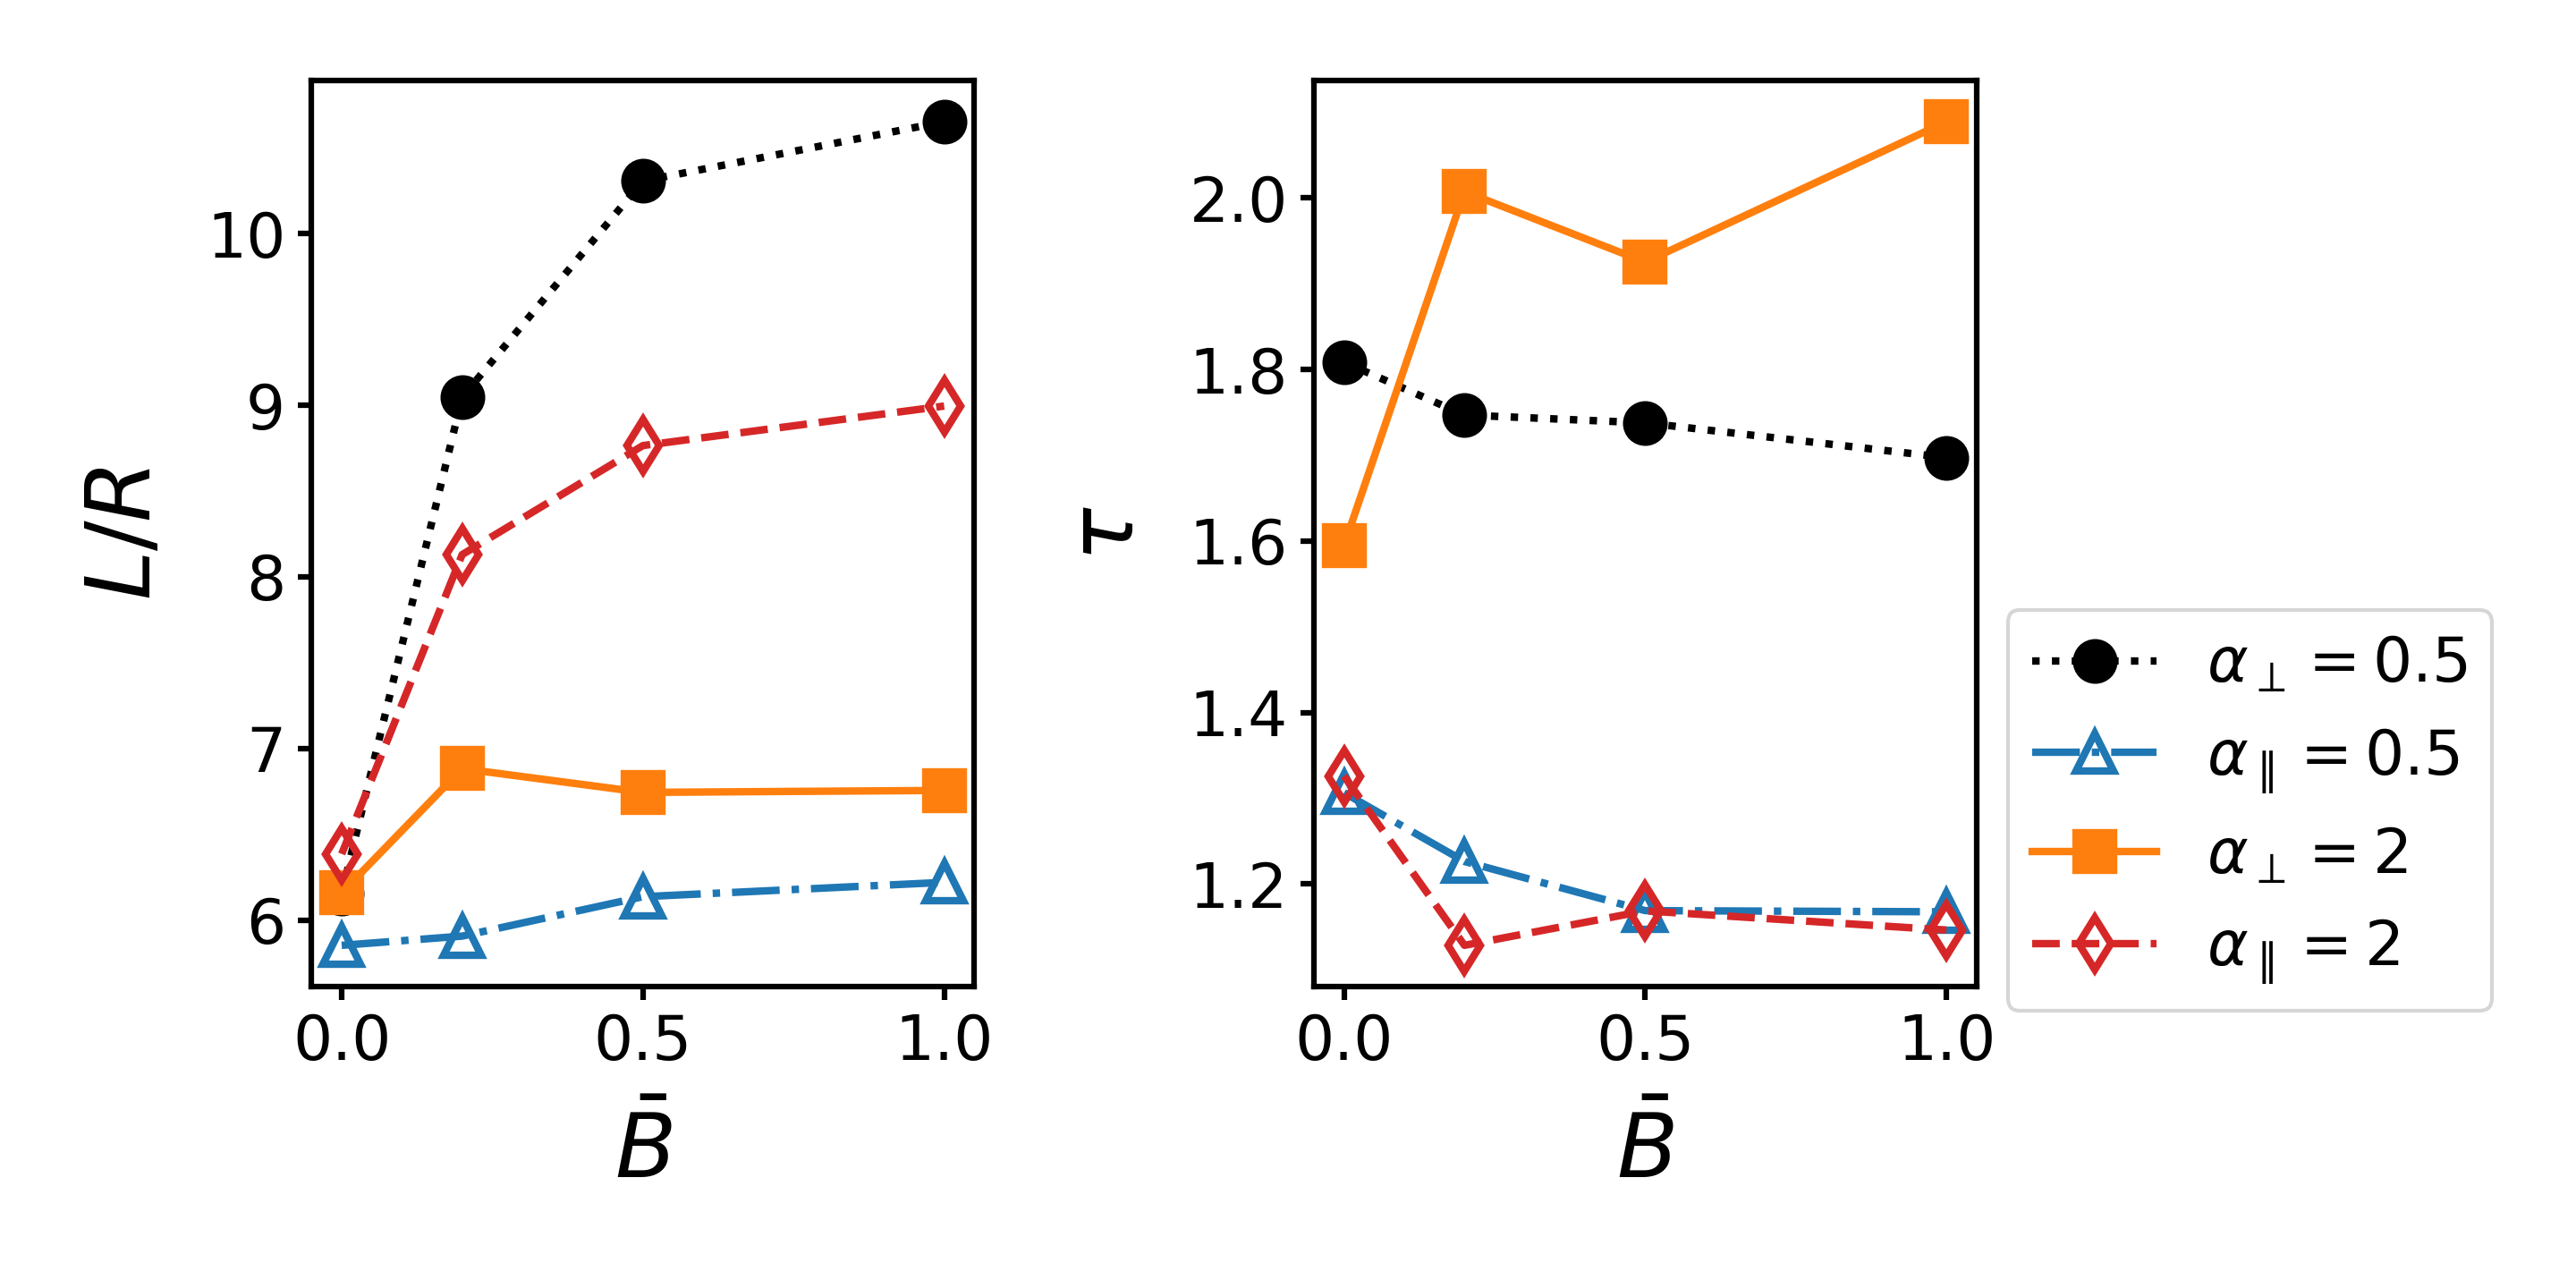
\includegraphics[scale=0.5]{../figures/results/paper2/domain_size_aniso-field_on.png} 
\caption{Plotting the anisotropic domain size and tortuosities against the applied magnetic field strength on the left and right respectively for bijels 
         stabilized with magnetically responsive oblate and prolate ellipsoids. We see that upon application of the field, bijels stabilized with prolate 
         particles experience a domains ize increase in the direction parallel to the applied field direction, $L_{\parallel}$, while the domain size 
         perpendicular to the applied field, $L_{\perp}$ decreases. The opposite is true for bijels stabilized with oblate particles. The tortuosity data 
         demonstrate that as the domain size increases, the tortuosity decreases and vice versa.} 
\label{fig:domain_size_aniso-field_on} 
\end{figure}

From Figure \ref{fig:domain_size_aniso-field_on}, domain size anisotropy is observed upon application of the field for both
particle morphologies. Some domain anisotropy with no applied field is observed, which increases upon application of the magnetic field.
The directional domain sizes, $L_{\perp}$ and $L_{\parallel}$ increase by 73\% and 7\%\ respectively for oblate particles and
10\% and 44\% respectively for oblate particles. The axes that coarsens the most is consistent with past work, explained through the
directions particles reorient in response to the applied magnetic field. As particles unjam and rejam at the interface due to reorientating 
to the magnetic field, they adopt direction specific surface coverages which manifest as anistropic domains upon jamming. In Figure 
\ref{fig:domain_size_aniso-field_on}, we demonstrate that the application of the magnetic field changes the domain size. 

The tortuosity of the bijel is initially around $\tau \approx 1.5$, consistent with simulations of the diffusive tortuosities of gyroid structures using 
Lattice Boltzmann simulations. \cite{luo_macroscopic_2020} Upon application of the field, $\tau_{\perp}$ slightly decreases while $\tau_{\parallel}$
increases. In Chapter \ref{chapter:aim1}, we characterized that increasing the domain size decreases the tortuosity. \cite{karthikeyan_formation_2024} This
observation is in line with the domain size changes observed in Figure \ref{fig:domain_size_aniso-field_on}. The results show that the
tortuosity of the bijel is noticeably affected by the application of magnetic fields. This data suggests that magnetic fields applied onto
bijels stabilized with ellipsoidal particles undergo domain anisotropy upon application of magnetic fields. However the particle morphology,
specifically its axis of symmetry, affect the direction that the domain anisotropy is characterized.

Next, we investigate the time gap between the average domain size increase and the nematic order parameter. This result suggests that the dynamics 
of the system at higher magnetic field strengths are dependent upon other factors that vary upon application of the magnetic field. In this system, these factors
would arise from capillary forces with the interface or steric interactions with other particles at the interface, slowing down the dynamics of the system.
To understand this phenomena, we focus on the dynamics of the particle monolayer. First, we visualize the particle monolayer of the bijels stabilized with prolate 
ellipsoids at the initial and final configuration before and after application of a magnetic field.

\begin{figure} 
\centering 
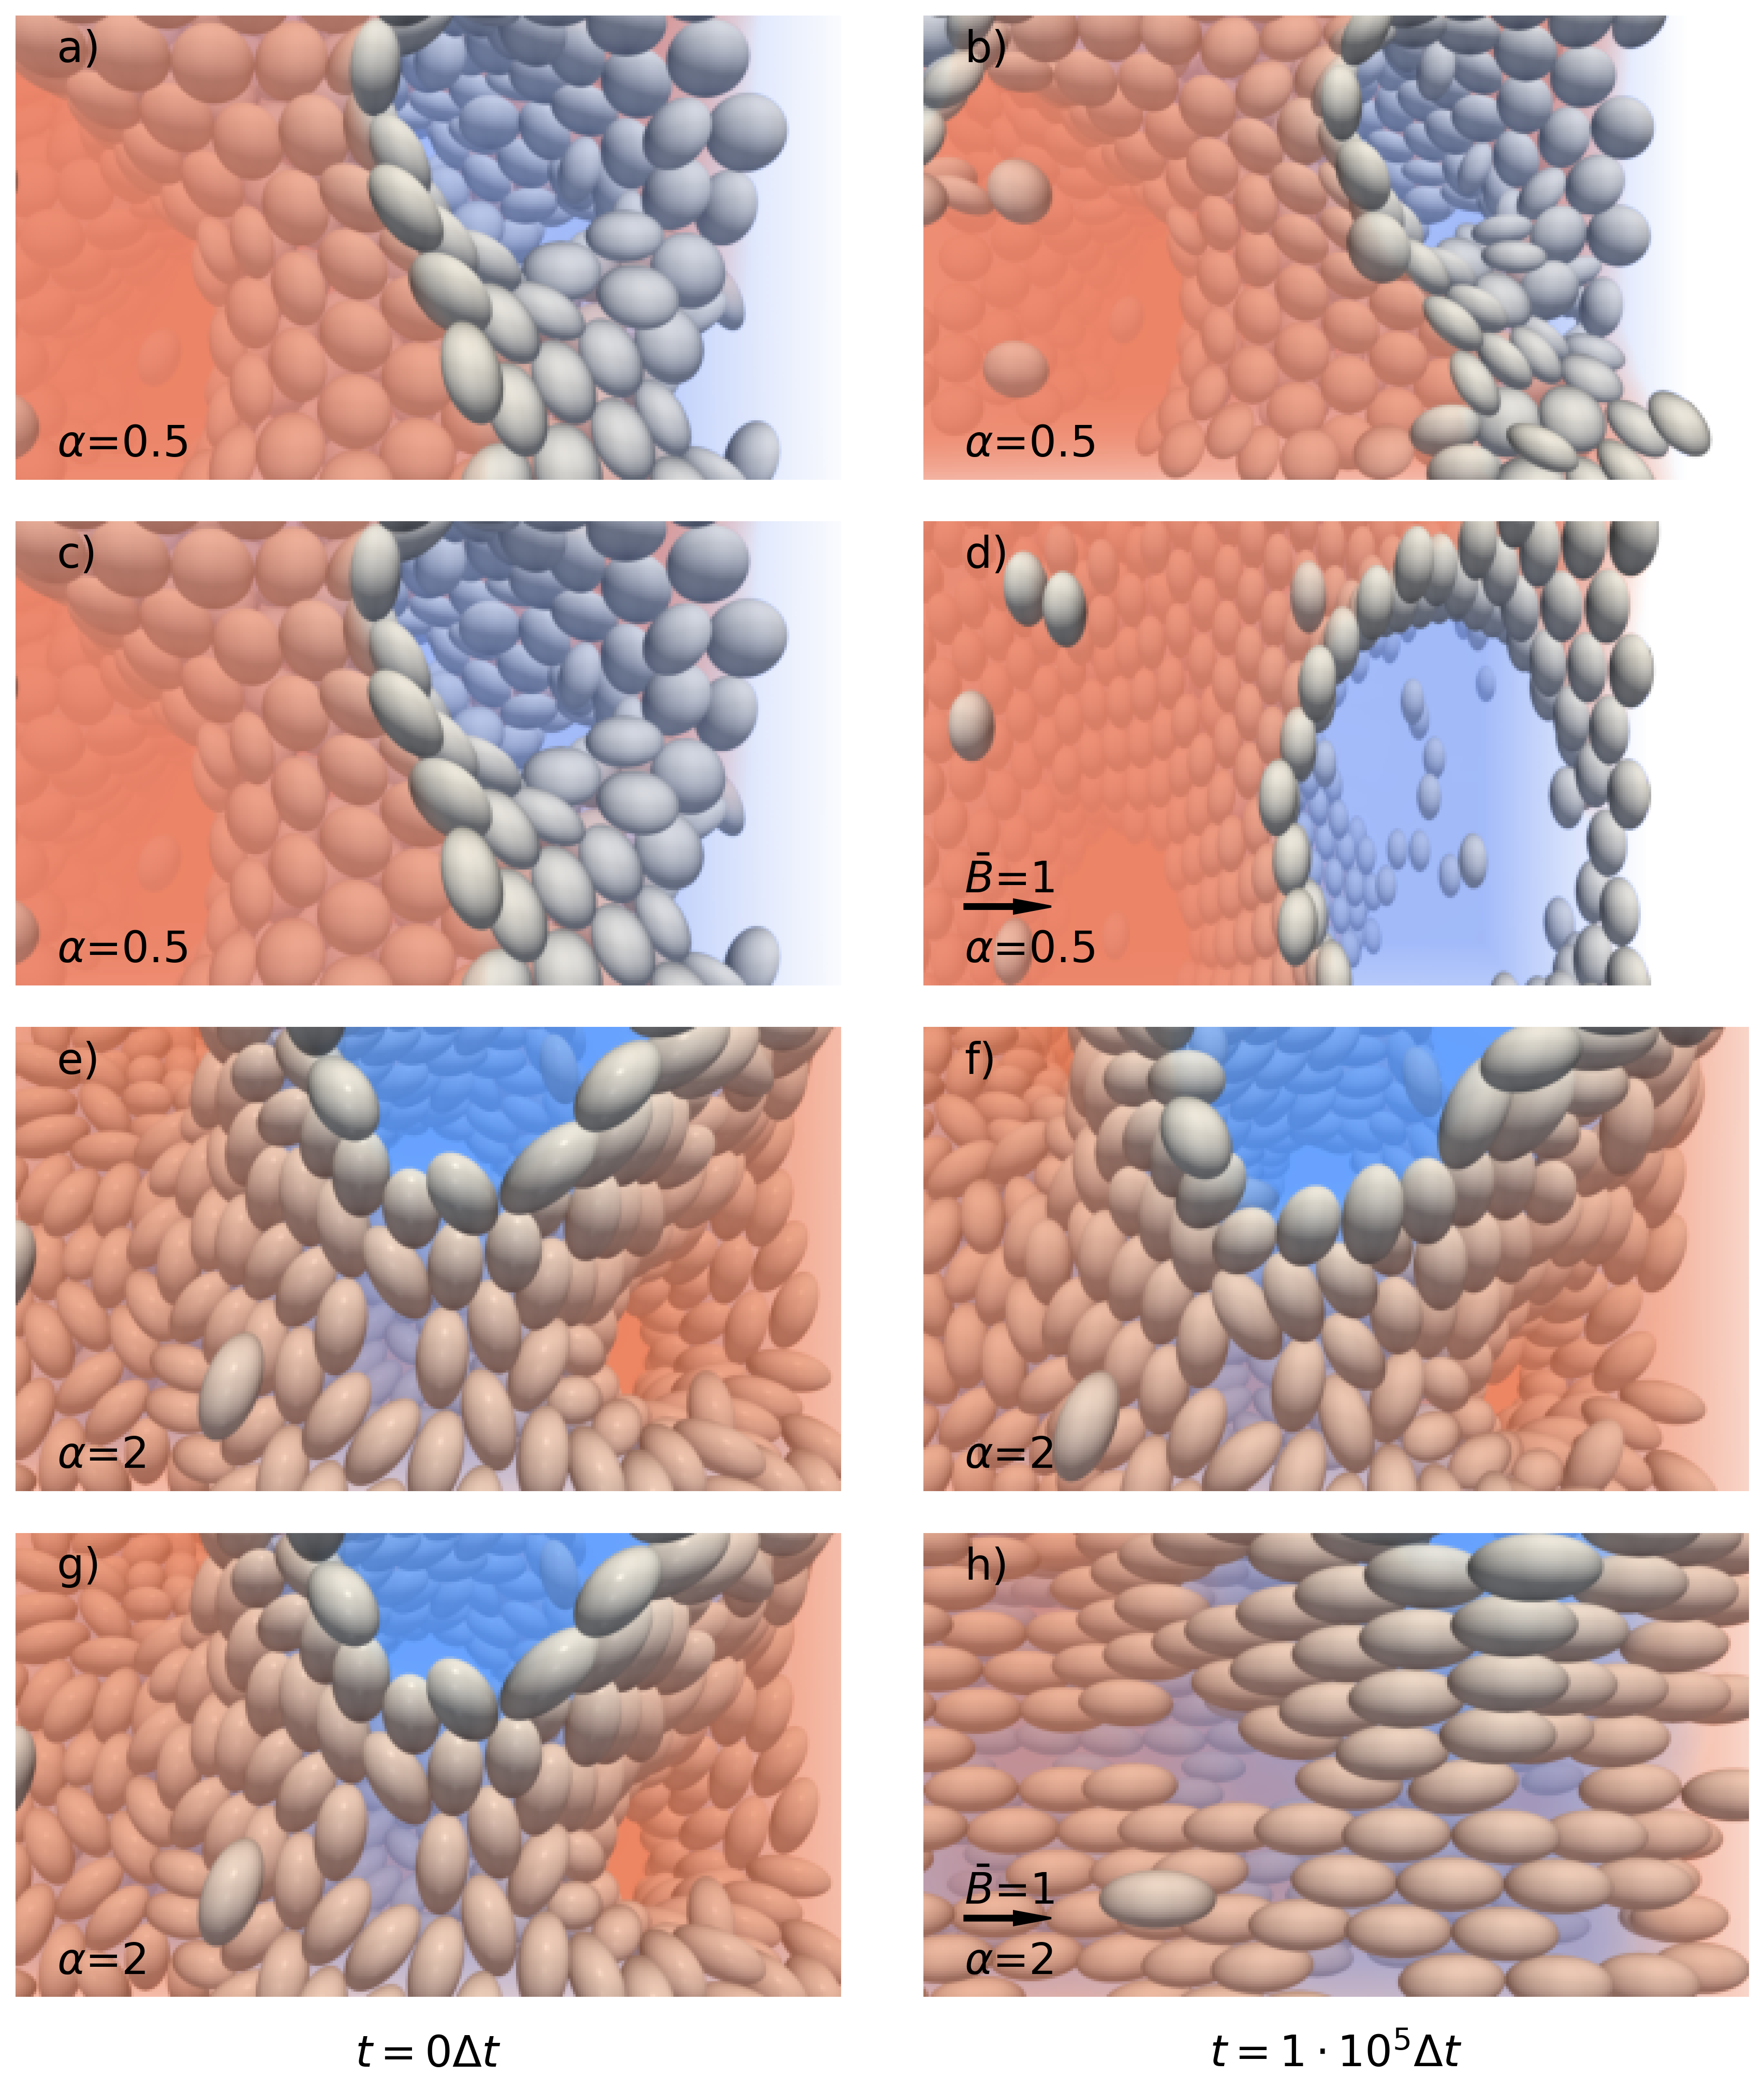
\includegraphics[scale=0.2]{../figures/results/paper2/particle_viz-field_on.png} 
\caption{Visualizations of bijels stabilized with oblate and prolate particles simulated at $t = 0$ (left column) and $t = 10^5$ (right column). The first and 
         third rows show the particle monolayer of bijels stabilized with oblate and prolate ellipsoids respectively with no applied field. The second and fourth 
         rows show the particle monolayer of bijels stabilized with oblate and prolate ellipsoids respectively with an applied field of $\bar{B}_z = 1$. Particle 
         reorientation to the direction of the field can be seen, resulting in coarsening of the domains.} 
\label{fig:particle_viz-field_on} 
\end{figure}

In Figure \ref{fig:particle_viz-field_on}, we see the initial configuration of particles at the monolayer show that the orientations are random and that the 
particles tend to lie flat on the interface. However, upon application of the magnetic field the particles orient to the field direction. With no applied field,
the orientations and positions of the particles vary slightly for both ellipsoidal particle morphologies. This effect is due steric effects between particles,
as identified in Gunther et al. \cite{gunther_timescales_2014} Bijels stabilized by prolate ellipsoids, adopt orientational order
to the magnetic field and qualitatively different particle arrangements on the interface. These indicate that the interfacial capillary forces or steric interactions 
with other particles differ upon application of the magnetic field. The particles would prefer to lie flat on the interface to minimize the interfacial energy of 
adsorption onto the interface. Changes in the local arrangement arise from the unjamming and rejamming process upon application of the magnetic field. These differences 
in the orientational and interfacial ordering can be characterized to understand how each respective interaction force changes as a function of time.

Bresme and Faraudo and Davies investigating the reorientation of particles at interfaces under magnetic fields have shown that a critical magnetic field exists, 
above which the particle orients to the field and below which the particle orientation is a function of the capillary force and magnetic field derived force. 
\cite{davies_interface_2014} \cite{bresme_orientational_2007} Particle adsorption into the interface with microparticles have also been shown to be irreversible due 
to the high adsorption energy. Upon particle reorientation, the microstructure change can be driven solely through particle unjamming and re-jamming, or it can be 
driven through the particles dragging the interface during this process. The mechanism of unjamming and re-jamming can be investigated using the average interfacial 
angle, $\langle \psi \rangle$ and the local ordering of the particles characterized with  $\langle Q6 \rangle$ Past work has identified that local crystallization 
of colloidal supercooled fluids takes place at \(\langle Q6 \rangle = 0.38\). \cite{toxvaerd_role_2020} Past investigations into the rheology of bijels have revealed
that bijels are colloidal glasses percolating in 3D space. \cite{ching_bijel_2022} However, application of a magnetic field results in reorientation of particles on
the interface that can temporarily reduce the interfacial coverage of the particles on the interface, temporarily making the particle monolayer more liquid-like
than amorphous. \cite{hunter_physics_2012} Using this approximation, we can use the local crystallization result shown in Toxvaerd.

\begin{figure} 
\centering 
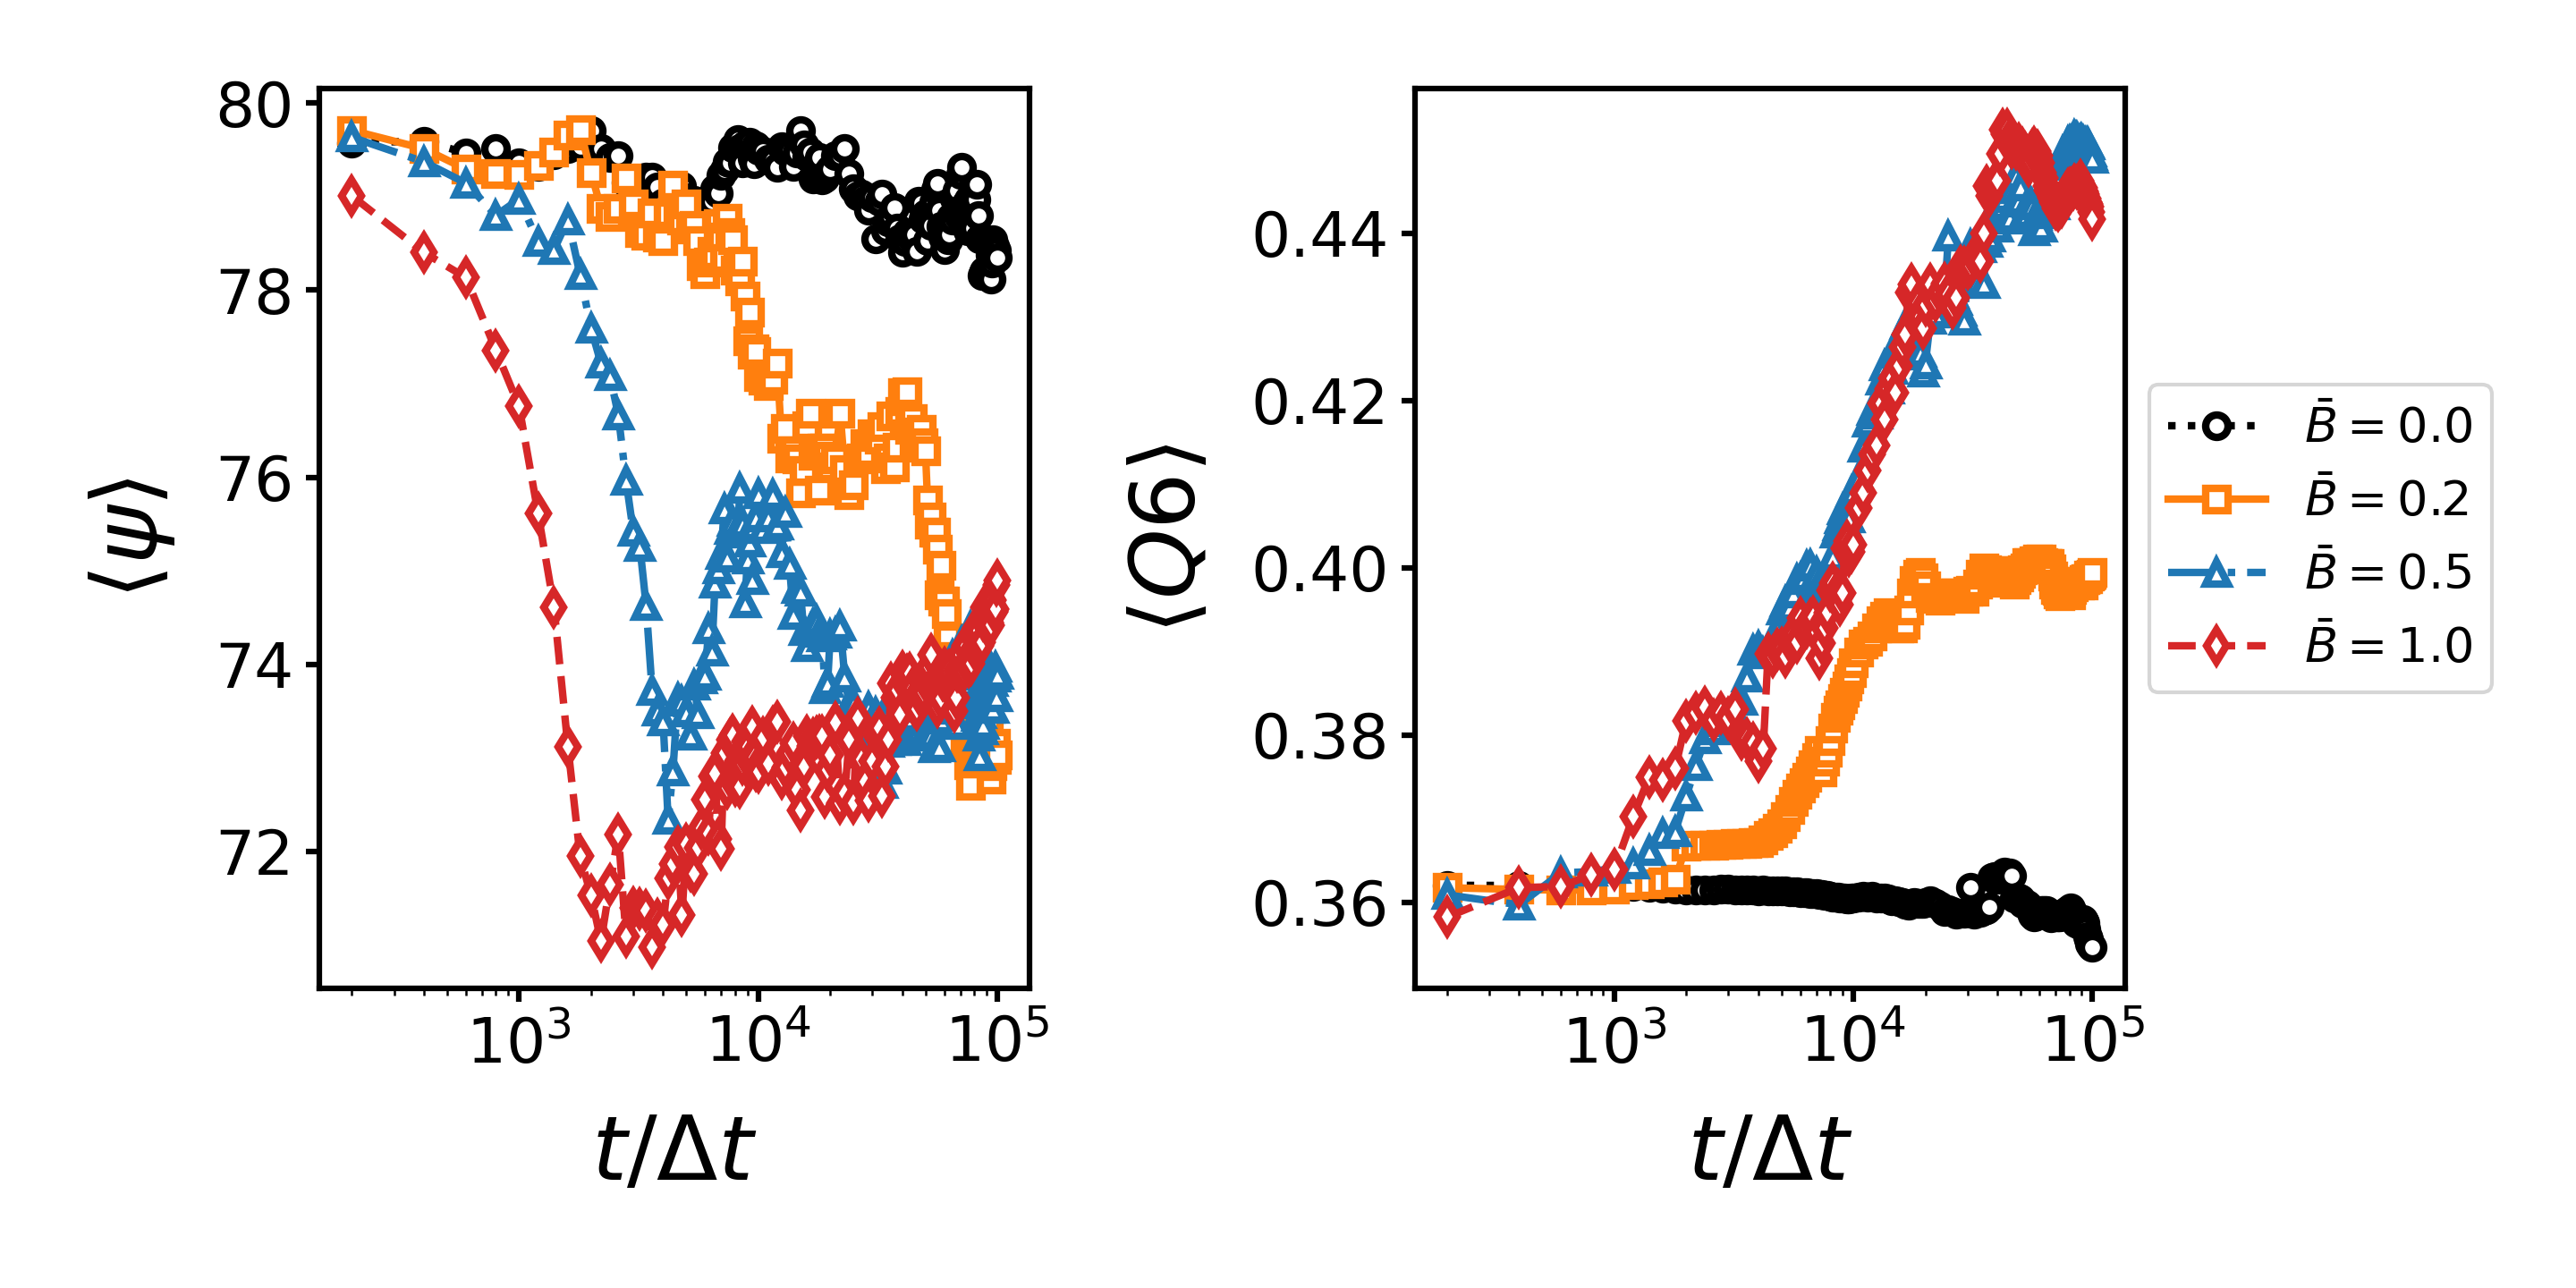
\includegraphics[scale=0.5]{../figures/results/paper2/interface_angle-nint-field_on.png} 
\caption{Plots of the interface angle $(\langle \psi \rangle)$ and six fold Steinhardt order parameter $(\langle Q6 \rangle)$ on the left and right respectively, 
         versus time for bijels stabilized with oblate and prolate ellipsoids on the top and bottom rows respectively. I demonstrate that upon application 
         of a magnetic field, the behavior of $(\langle \psi \rangle)$ and $(\langle Q6 \rangle)$ differ significantly between oblate and prolate ellipsoids 
         indicating that the dynamics for both particle morphologies differ. I also observe magnetic field dependence in each property for both particle types, 
         suggesting that these changes are driven primarily through the change in the applied field strength.} 
\label{fig:interface_angle-nint-field_on} 
\end{figure}

From Figure \ref{fig:interface_angle-nint-field_on}, we identify that prolate and oblate particles respond differently at the interface. For
bijels stabilized by oblate ellipsoids, we characterize an increase in $\langle \psi \rangle$ from an initial value of $19 ^{\circ}$,
before it reduces slightly and begins to increase once again. The initial starting value of $\langle \psi \rangle$ indicates the
particles are lying close to flat on the interface, before they begin to tilt out of the interface when the magnetic field is applied. Then,
$\langle \psi \rangle$ plateaus as the interface begins to move in response to the tilting particle at the interface. This is caused by the
large adsorption energy of the particles at the interface of the bijel, caused by high surface tension. Finally, the particles jam in place,
locking the interface at an angle to the particle. The rate of increase in $\langle \psi \rangle$ at early stages and the time spent
in the plateau increase with a larger applied magnetic field. The final angle at the interface is also dependent upon the applied field
strength.

When analyzing $\langle \psi \rangle$ for bijels stabilized by prolate particles, this behavior can also be observed. $\langle \psi \rangle$
begins at $10 ^{\circ}$. $\langle \psi \rangle$ increases, before plateauing and slowly decreasing. The initial peak height and rate of increase in 
$\langle \psi \rangle$ is field dependent, although given the small decrease in $\langle \psi \rangle$ it is unclear if the final value of this parameter 
is field dependent for bijels stabilized with prolate particles. The changes in $\langle \psi \rangle$ for bijels stabilized with prolate particles are 
small compared to bijels stabilized with oblate particles. We visualize this process by color coding snapshots of the particle monolayer at the initial
and final timesteps of bijels stabilized by prolate particles with a field strength of $\bar{B} = 1$ applied.

\begin{figure} 
    \centering 
    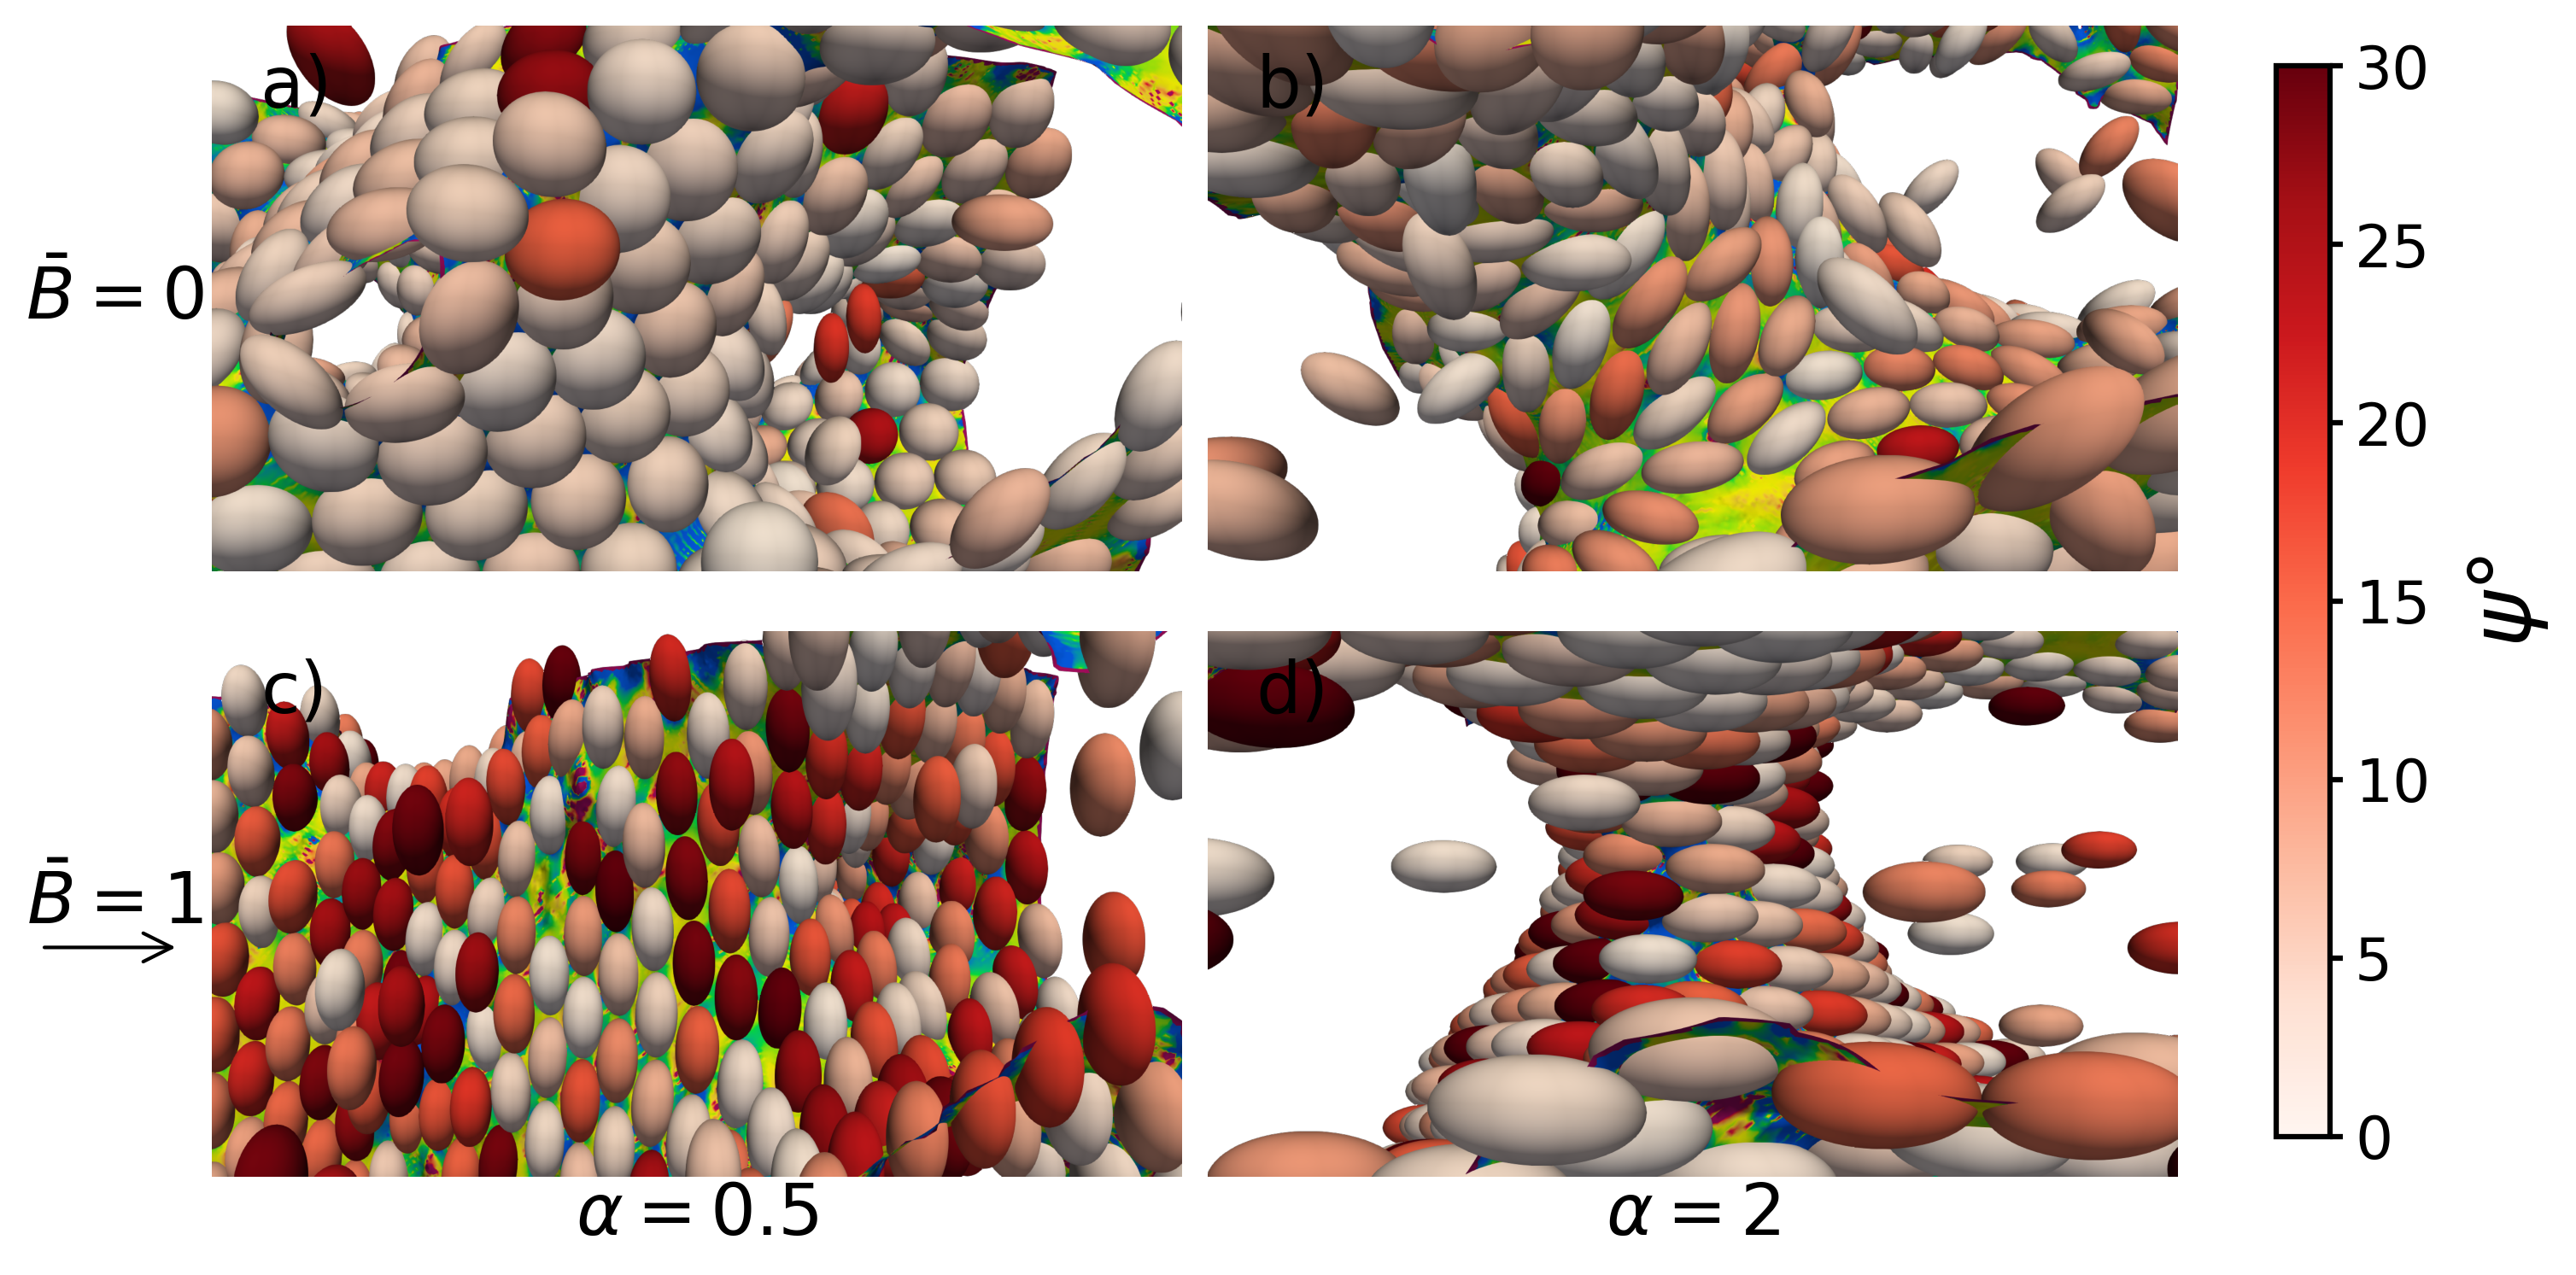
\includegraphics[scale=0.4]{../figures/results/paper2/psi_concat_startB-0_endB-1.png} 
    \caption{Visualizations of bijel stabilized by ellipsoidal particles made with no applied field having a field strength of $\bar{B} = 1$ applied. The top and bottom 
             rows show $\psi$ for each particle at the initial and final timesteps respectively.The intensity
             of the red color qualitatively indicates the magnitude of the $\psi$ for each particle. Field application causes particles to flip out of the interface for
             oblate particles, while prolate particles tilt out of the interface. The interface is shaded with the Gaussian curvature.} 
    \label{fig:psi_field_on_visualize} 
\end{figure}

From the visualizations in Figure \ref{fig:psi_field_on_visualize}, the particles lie mostly flat on the interface at the initial timestep. Upon application of a field 
strength of $\bar{B} = 1$, the final state of the monolayer is particle morphology dependent. Oblate particles tend to flip on the interface into a metastable state where
the interface covered by each particle is done with the $R_p$ and $R_o$ compared to its lowest energy state where it lies flat with radii $R_o$. The particle monolayer
of bijels stabilized by prolate particles tilt out of the interface with no metastable configurations observed. This effect explains the trends seen in $\langle \psi \rangle$
at long times for both particle morphologies. This particle flipping on the interface affects the way the particles can arrange on the interface, like what we 
characterized In Figure \ref{fig:rdf}. This change in local ordering can be quantified using $\langle Q6 \rangle$.

From Figure \ref{fig:interface_angle-nint-field_on} the dynamics of $\langle Q6 \rangle$ are particle morphology specific but can be split into three sections for 
both particle morphologies. Characterizing the time evolution of $\langle Q6 \rangle$ for oblate particles, we see a decrease upon application of the magnetic field, 
followed by a plateau and finally a gradual increase before jamming takes place, seen as a significant decrease in the rate of chang to $\langle Q6 \rangle$.
These results indicate that the ordering of the particles is reduced by the applied magnetic field, before a
restoration of some of the pre-existing order. The final values of $\langle Q6 \rangle$ are magnetic field dependent, with a stronger
magnetic field having a lower final $\langle Q6 \rangle$ value indicating that either the ordering of particles influence the angle at
the interface or vice versa. 

We observe that for bijels stabilized by prolate particles, the interface ordering of the particles increases as a
function of the applied field strength. The first phase of the evolution of $\langle Q6 \rangle$ sees some growth in $\langle Q6 \rangle$ before 
increasing dramatically and plateauing as jamming takes place. The length of time of the initial plateau and growth regions are negatively and
positively correlated to the applied magnetic field strength. Upon application of the magnetic field, $\langle Q6 \rangle > 0.38$ in all cases. Approximating
the particle monolayer as a colloidal glass that underwent a glass transition, the monolayer can be said to undergo a local crystallation event when 
$\langle Q6 \rangle > 0.38$. \cite{toxvaerd_role_2020}

Thus far, three particle based phenomena have been characterized; the orientation of the particle to the magnetic field, the interface and the local 
arrangement of the particles on the interface. we can calculate a timescale for each factor from the plots of each of these properties.
The nematic order parameter $S$ represents the ordering of
particles to an average direction, which in the case of the application
of a magnetic field, is the field direction. Therefore, a timescale
reliant on the nematic order parameter would represent a timescale of
response rate limited to the response to the magnetic field, which
indicates a particle-field orientation dependence named $\tau_S$. When applying a field to a bijel system with a
randomly oriented particle monolayer, the most significant transition
point is the isotropic to nematic transition or when $S \geq 0.3$. We
define $\tau_S$ as the the isotropic to nematic transition point.

We can also do the same for $\langle \psi \rangle$ and
$\langle Q6 \rangle$. A timescale derived from
$\langle \psi \rangle$ named $\tau_{\langle \psi \rangle}$
represents the capillary timescale between the interface and the
particle. Given the shape of the plot, we assign
$\tau_{\langle \psi \rangle}$ to be the time when the first minimum of
$\langle \psi \rangle$ is observed for prolate particles and the first
maximum for oblate particles. A timescale derived from
$\langle Q6 \rangle$, named $\tau_{\langle Q6 \rangle}$ is also
calculated which represents a timescale of local particle rearrangement.
We define $\tau_{\langle Q6 \rangle}$ as the time when
\(\langle Q6 \rangle \geq 0.38\) for prolate particles and the global
minimum of $\tau_{\langle Q6 \rangle}$ for the oblate particles. I
omit \(\bar{B} = 0\) as previous results have identified the domain size
changes observed there. We then plot the average domain size $L$
against time rescaled with these three timescales in Figure
\ref{fig:domain_size-field_on-scaled}.

\begin{figure} 
\centering 
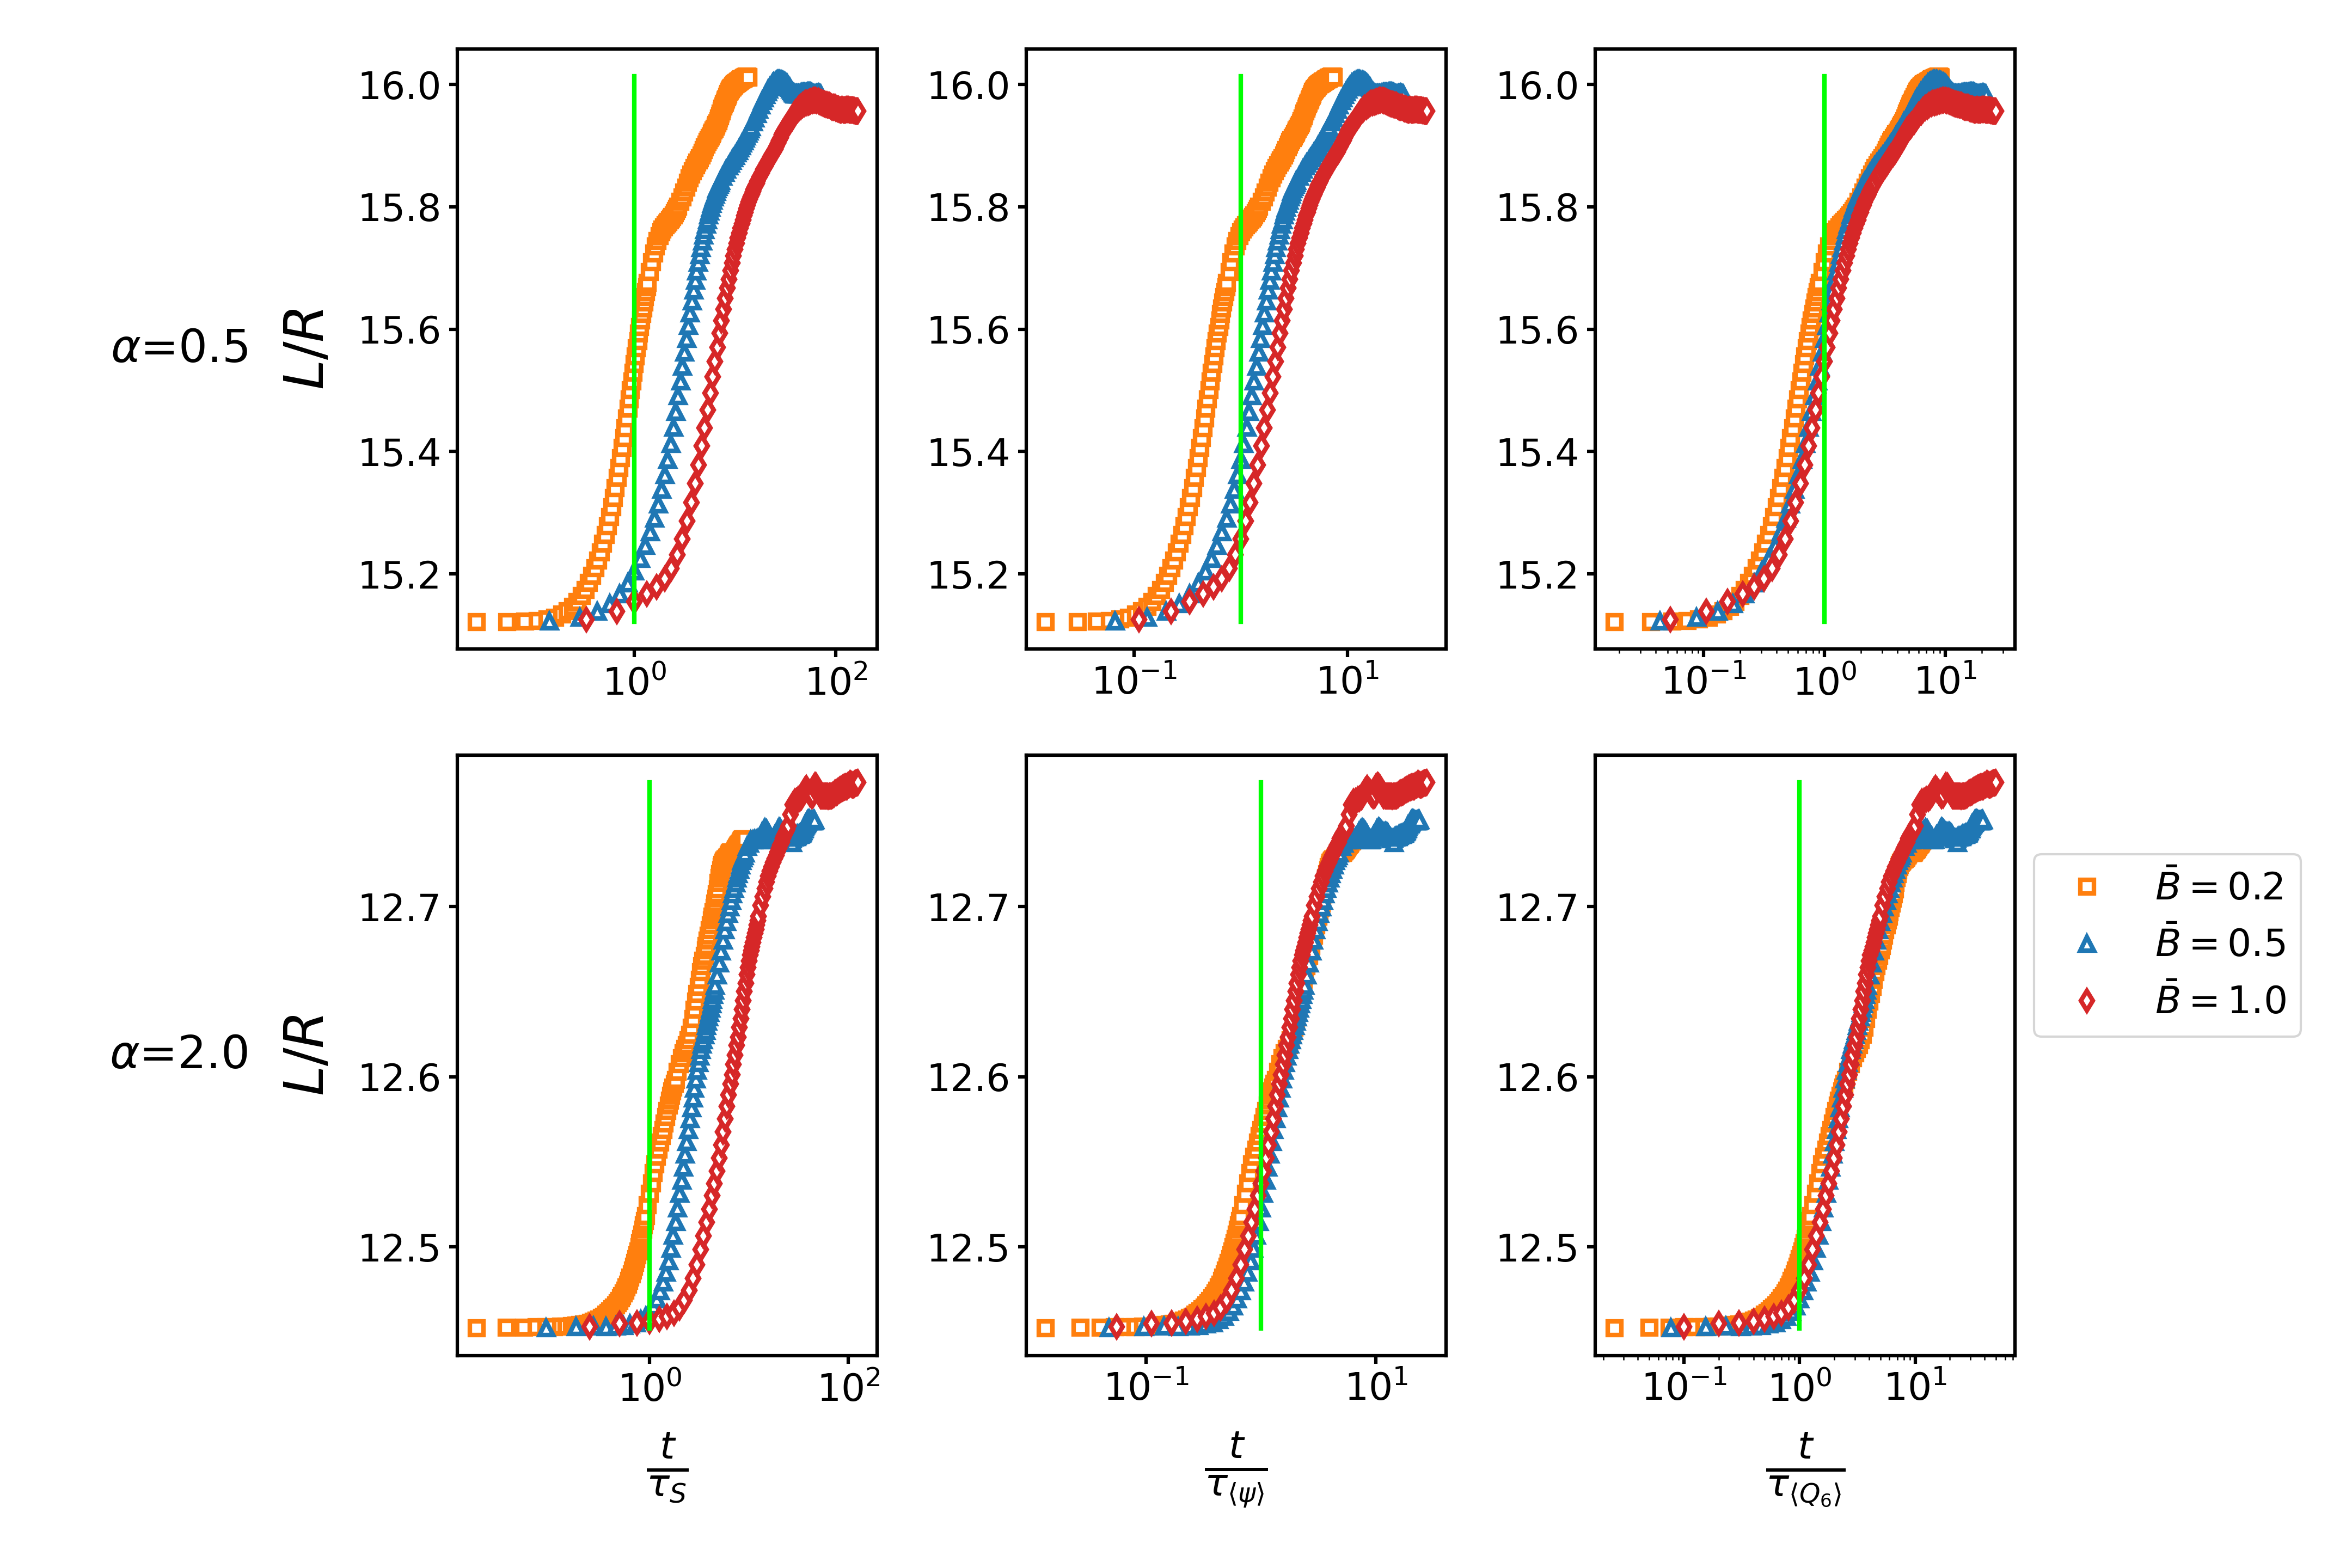
\includegraphics[scale=0.4]{../figures/results/paper2/domain_size-field_on-scaled.png} 
\caption{Plots of domain size with different timescales. The top and bottom row represent the average domain size for bijels stabilized with oblate and 
         prolate particles respectively. The figures on the left plots the domain size against time rescaled with the nematic to isotropic transition time, 
         $\tau_S$. The figures in the middle plot the domain size against time rescaled with the interfacial capillary timescale, $\tau_{\langle \psi \rangle}$. 
         The figures on the right plot the domain size against time rescaled with the particle rearrangement timescale, $\tau_{\langle Q6 \rangle}$. We show 
         that the controlling timescale when applying a magnetic field onto bijels with disordered particles is the latter timescale, indicating that the 
         dominating effect is steric hindrance of the particles during rearrangment at the interface.} 
\label{fig:domain_size-field_on-scaled} 
\end{figure}

In Figure \ref{fig:domain_size-field_on-scaled}, the left plot plots the
average domain size against time rescaled using $\tau_S$. The
the domain sizes do not collapse onto a single line, which is expected
if we want to explain the dynamics using the nematic order parameter.
This confirms the observation made above that the dynamics do not only
depend on the reorientation of particles to the field. The middle plot
demonstrates the average domain size against time rescaled using
$\tau_{\langle \psi \rangle}$. There is good agreement
between all simulations for prolate particles, although the point when
$\frac{t}{\tau_{\langle \psi \rangle}} = 1$ lies when the domain size
transition has started. However for oblate particles this
timescale does not describe the dynamics well.

The right plot demonstrates the domain size change after rescaling time
with $\tau_{\langle Q6 \rangle}$ all plots collapse onto a single line and 
the domain size transition also begins at
$\frac{t}{\tau_{\langle Q6 \rangle}} = 1$. The latter point
demonstrates that the dynamics for the structural response of randomly
oriented particles are controlled by the local particle rearrangement at
the interface rather than the orientation of the particle to the
magnetic field. As the dynamics of both particle morphologies are well described
using the particle steric effects timescale, denoted by $\tau_{\langle Q6 \rangle}$,
We conclude that the dynamics of bijels stabilized by ellipsoidal particles are controlled by
interfacial particle rearrangement at the interface.

From the evidence in Figure \ref{fig:domain_size-field_on-scaled}, two
types of interfacial behaviors are characterized in addition to that
identified by Gunther et al.~\cite{gunther_timescales_2014} The first
type is what is observed for $\bar{B} = 0.2$, where the interfacial
arrangement and orientation of the particle monolayer to the field and to the
interface change in lock step. This causes the interface to reorient at
the same rate as the particles reorienting to the magnetic field. The
second is observed for $\bar{B} = 0.5, 1$, where there is a time lag
between particle ordering, and the intiation of domain coarsening. In
the latter scenario, at early times the particles are jolted out of
position before the large adsorption energy of the particles into the
interface causes the interface to move to the particle position, causing
domain coarsening as the interfacial area reduces before rejamming reforms the bijel.

\subsection{Increasing the applied
field}\label{increasing-the-applied-field}

The hysteresis curve in Figured \ref{fig:hysteresis_curve} shiows that the microstructure change at higher
field strengths began to reduce with each subsequent field strength
jump, suggesting that the ordering of the particles is linked to the
domain size change observed. In the previous section, We saw that domain
size changes in bijels after jamming are constrained by magnetic field
driven local rearrangement of the particle monolayer. In this section,
we explore how pre-existing order in the particles affect the degree of
domain size change observed. We apply fields of strength
$\bar{B}_{template} = 0, 0.2, 0.5, 1$ during phase separation to
create bijels stabilized with ellipsoidal particles with pre-existing
particle order. We then apply a field strength of $\bar{B}_z = 1$ and
observe the time evolution of the system for $t = 10^5$ timesteps. I
simplify my nomenclature here for brevity. For example,
$\bar{B}_z: 0.0 \rightarrow 1.0$ represents a bijel made with no
field, and a field of $\bar{B}_z = 1.0$ applied during the simulations conducted here. 
We begin by visualizing the microstructure
changes experienced by bijels simulated with pre-existing particle order
in Figure \ref{fig:microstructure_viz-field_up}.

\begin{figure}
\centering 
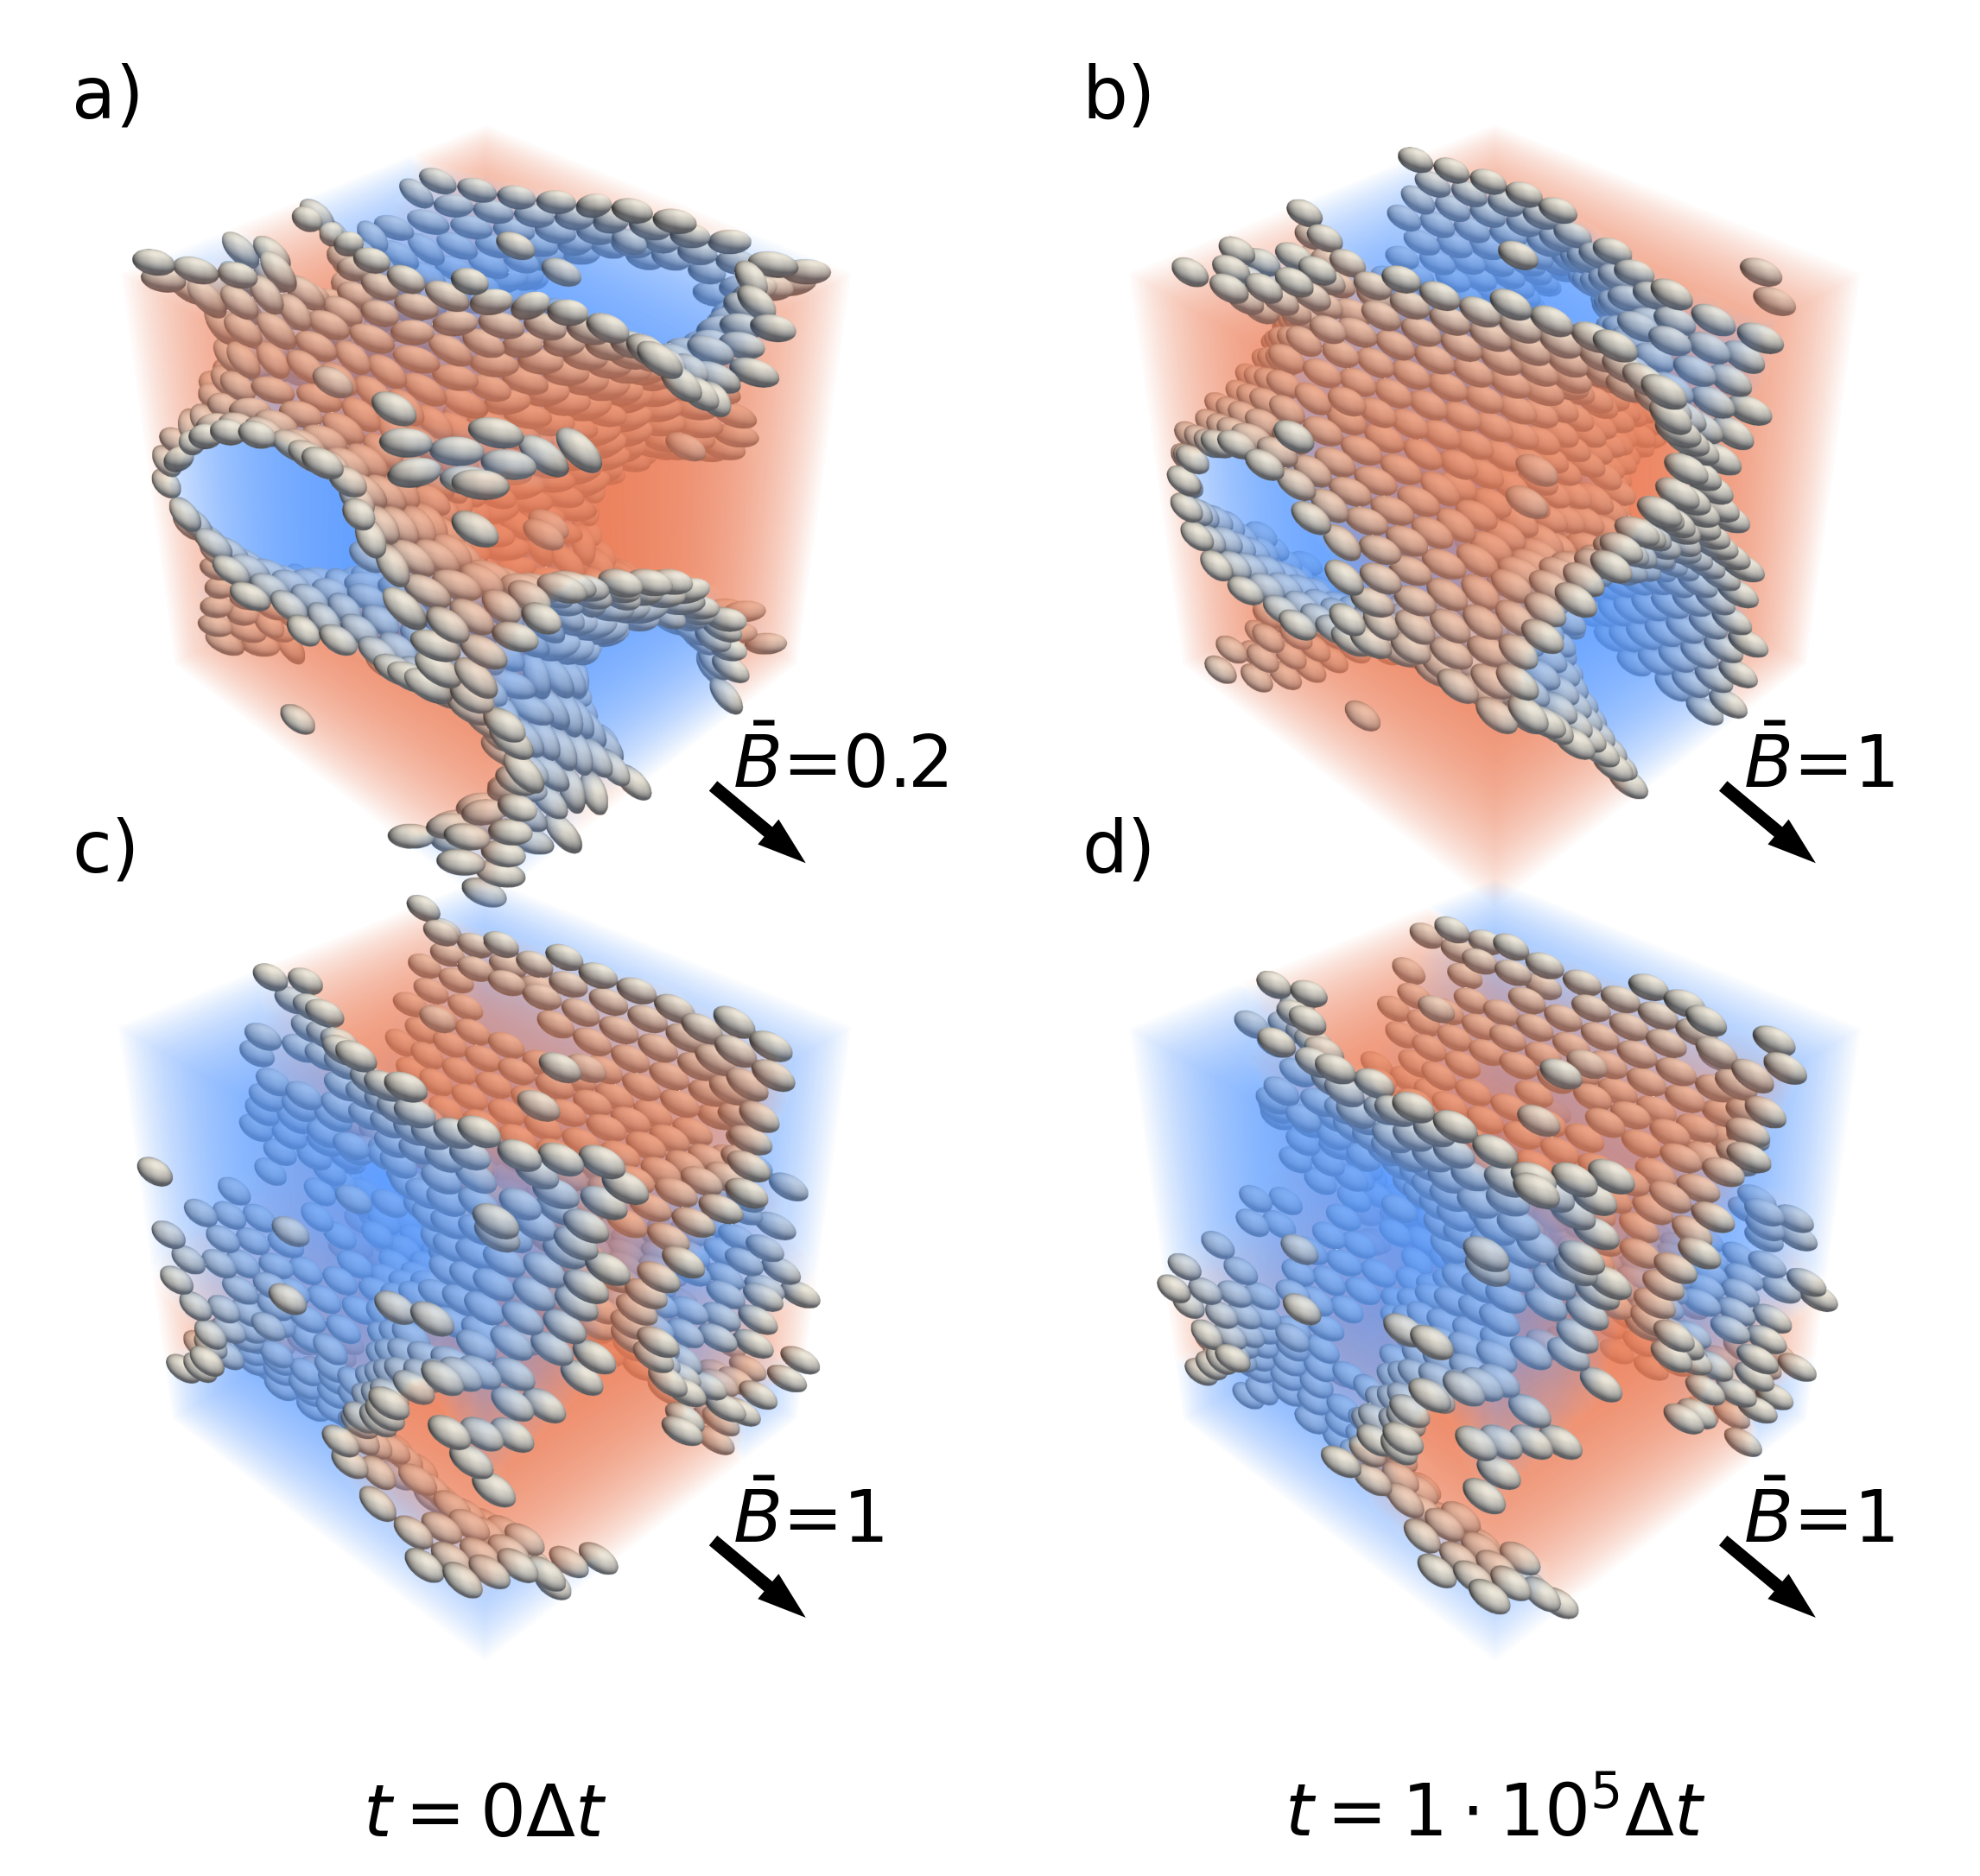
\includegraphics[scale=0.4]{../figures/results/paper2/microstructure_viz-field_up.png} 
\caption{Visualizations of bijels stabilized with oblate and prolate particles simulated at $t = 0$ (left column) and $t = 10^5$ (right column). 
         The first and third rows show the particle monolayer of bijels stabilized with oblate and prolate ellipsoids respectively with an applied 
         field of $\bar{B}_z = 0.2$. The second and fourth rows show the particle monolayer of bijels stabilized with oblate and prolate ellipsoids 
         respectively with an applied field of $\bar{B}_z = 1$. We increase the applied field to $\bar{B}_z = 1$ in both cases and show that particle 
         reorientation to the field occurs at the $\bar{B}_z = 0.2$ but not in the $\bar{B}_z = 1$ case.}
\label{fig:microstructure_viz-field_up}
\end{figure}

In Figure \ref{fig:microstructure_viz-field_up} We show representative
snapshots of a bijel stabilized with prolate particles at the initial
and final timestep with field conditions
$\bar{B}_z: 0.2 \rightarrow 1.0$ and
$\bar{B}_z: 1.0 \rightarrow 1.0$ in the top and bottom rows
respectively. We show that upon application of the field, the fluid
domains undergo a field strength dependent microstructrue response, with
the degree of response dependent upon the difference between the initial
and final magnetic field. We also observe a qualitative increase in the
alignment of the particles to the magnetic field for the
$\bar{B}_z: 0.2 \rightarrow 1.0$ case. We quantify these observations
by plotting the average domain size and nematic order parameter in
Figure \ref{fig:domain_size-field_up}.

\begin{figure} 
\centering 
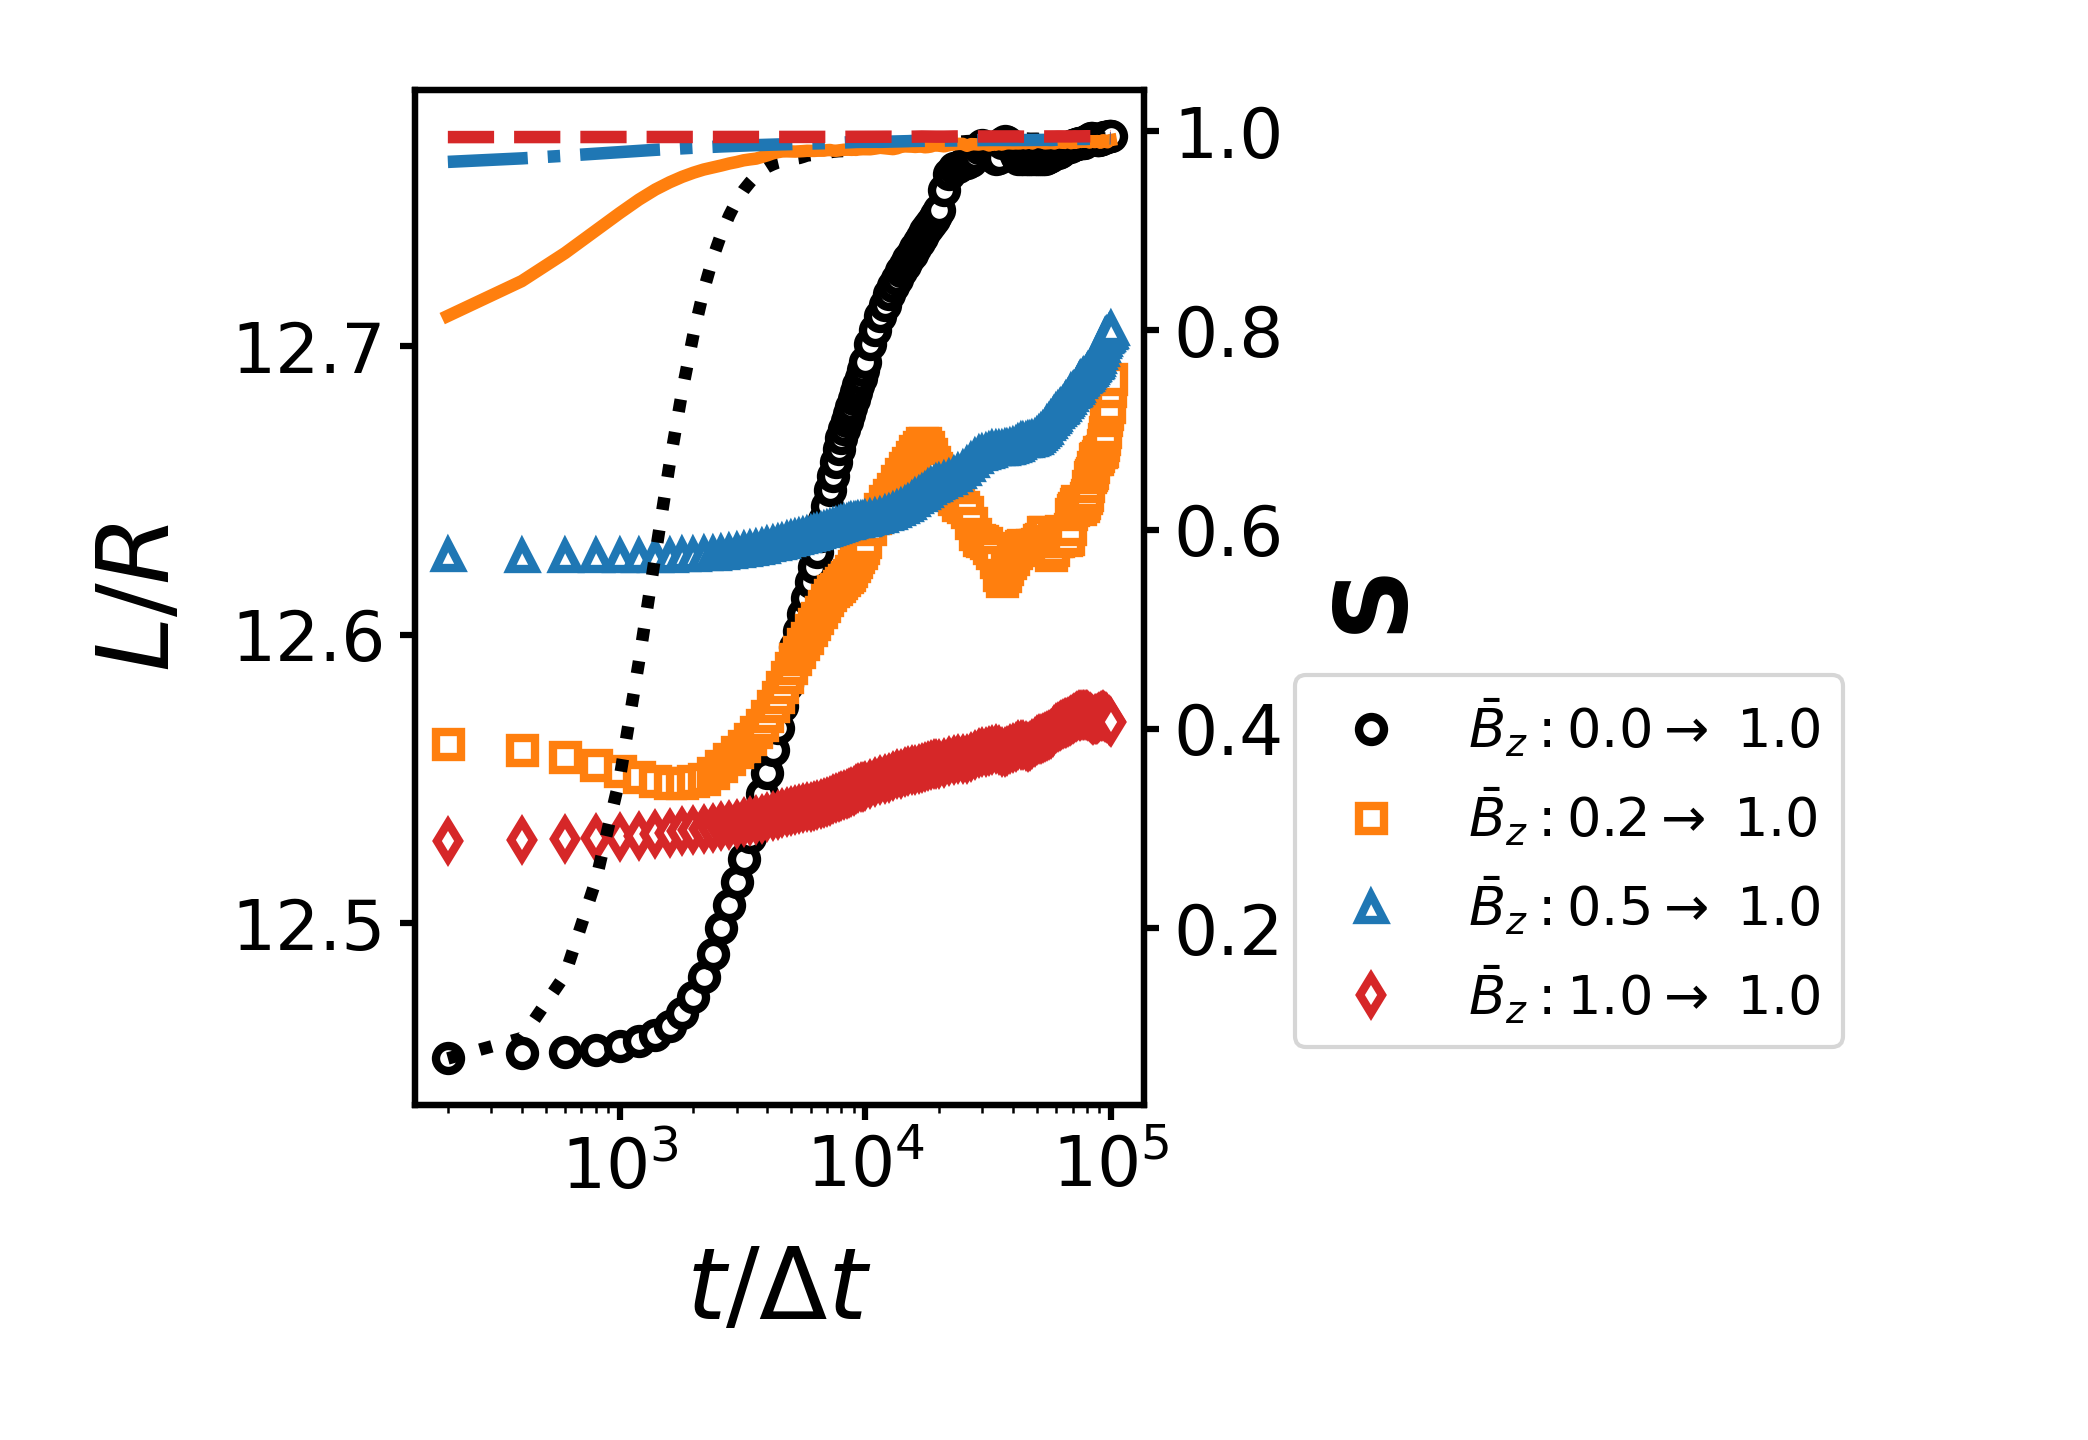
\includegraphics[scale=0.5]{../figures/results/paper2/domain_size-field_up.png} 
\caption{Plot of the spherically averaged domain size normalized with $Rp(L/R)$ of the particle in markers and the nematic order parameter in lines. 
         We show that the domain size change measured is correlated to the change in the particle ordering, characterized using the nematic order parameter.} 
\label{fig:domain_size-field_up} 
\end{figure}

In Figure \ref{fig:domain_size-field_up}, We define the difference
between the final and initial magnetic field strengths as
$\Delta \bar{B}$. The onset of microstructural response is observed to
be $\Delta \bar{B}$-dependent, indicating that a stronger driving
force is required to induce structural reorganization. Additionally, the
extent of microstructural change is also correlated with
$\Delta \bar{B}$, where $\Delta \bar{B} = 1$ results in average
microstructural variations of 5\% and 2\% for oblate and prolate
particles, respectively which decreases as $\Delta \bar{B}$ decreases.
We further characterize the relationship between $\Delta \bar{B}$ and
nematic order, showing that an increase in \(S\) correlates with
$\Delta \bar{B}$. This suggests that changes in domain size are
intrinsically linked to the initial particle ordering within the system.
These findings indicate that characteristic length scale evolution is
dependent on both aspect ratio and field strength variation,
highlighting the role of particle alignment in governing domain
coarsening dynamics. To further quantify the anisotropic microstructural
evolution, We define the relative change in domain size as
$\Delta L = \frac{L_{f} - L_{i}}{L_{i}}$, where $L$ represents
either $L_{\perp}$ or $L_{\parallel}$. The same formulation is
applied to the tortuosity in the respective directional components. I
do this to characterize the $\Delta \bar{B}$-dependent changes
observed in the domain anisotropy. The results are presented in Figure
\ref{fig:domain_size_aniso-field_up}.

\begin{figure} 
\centering 
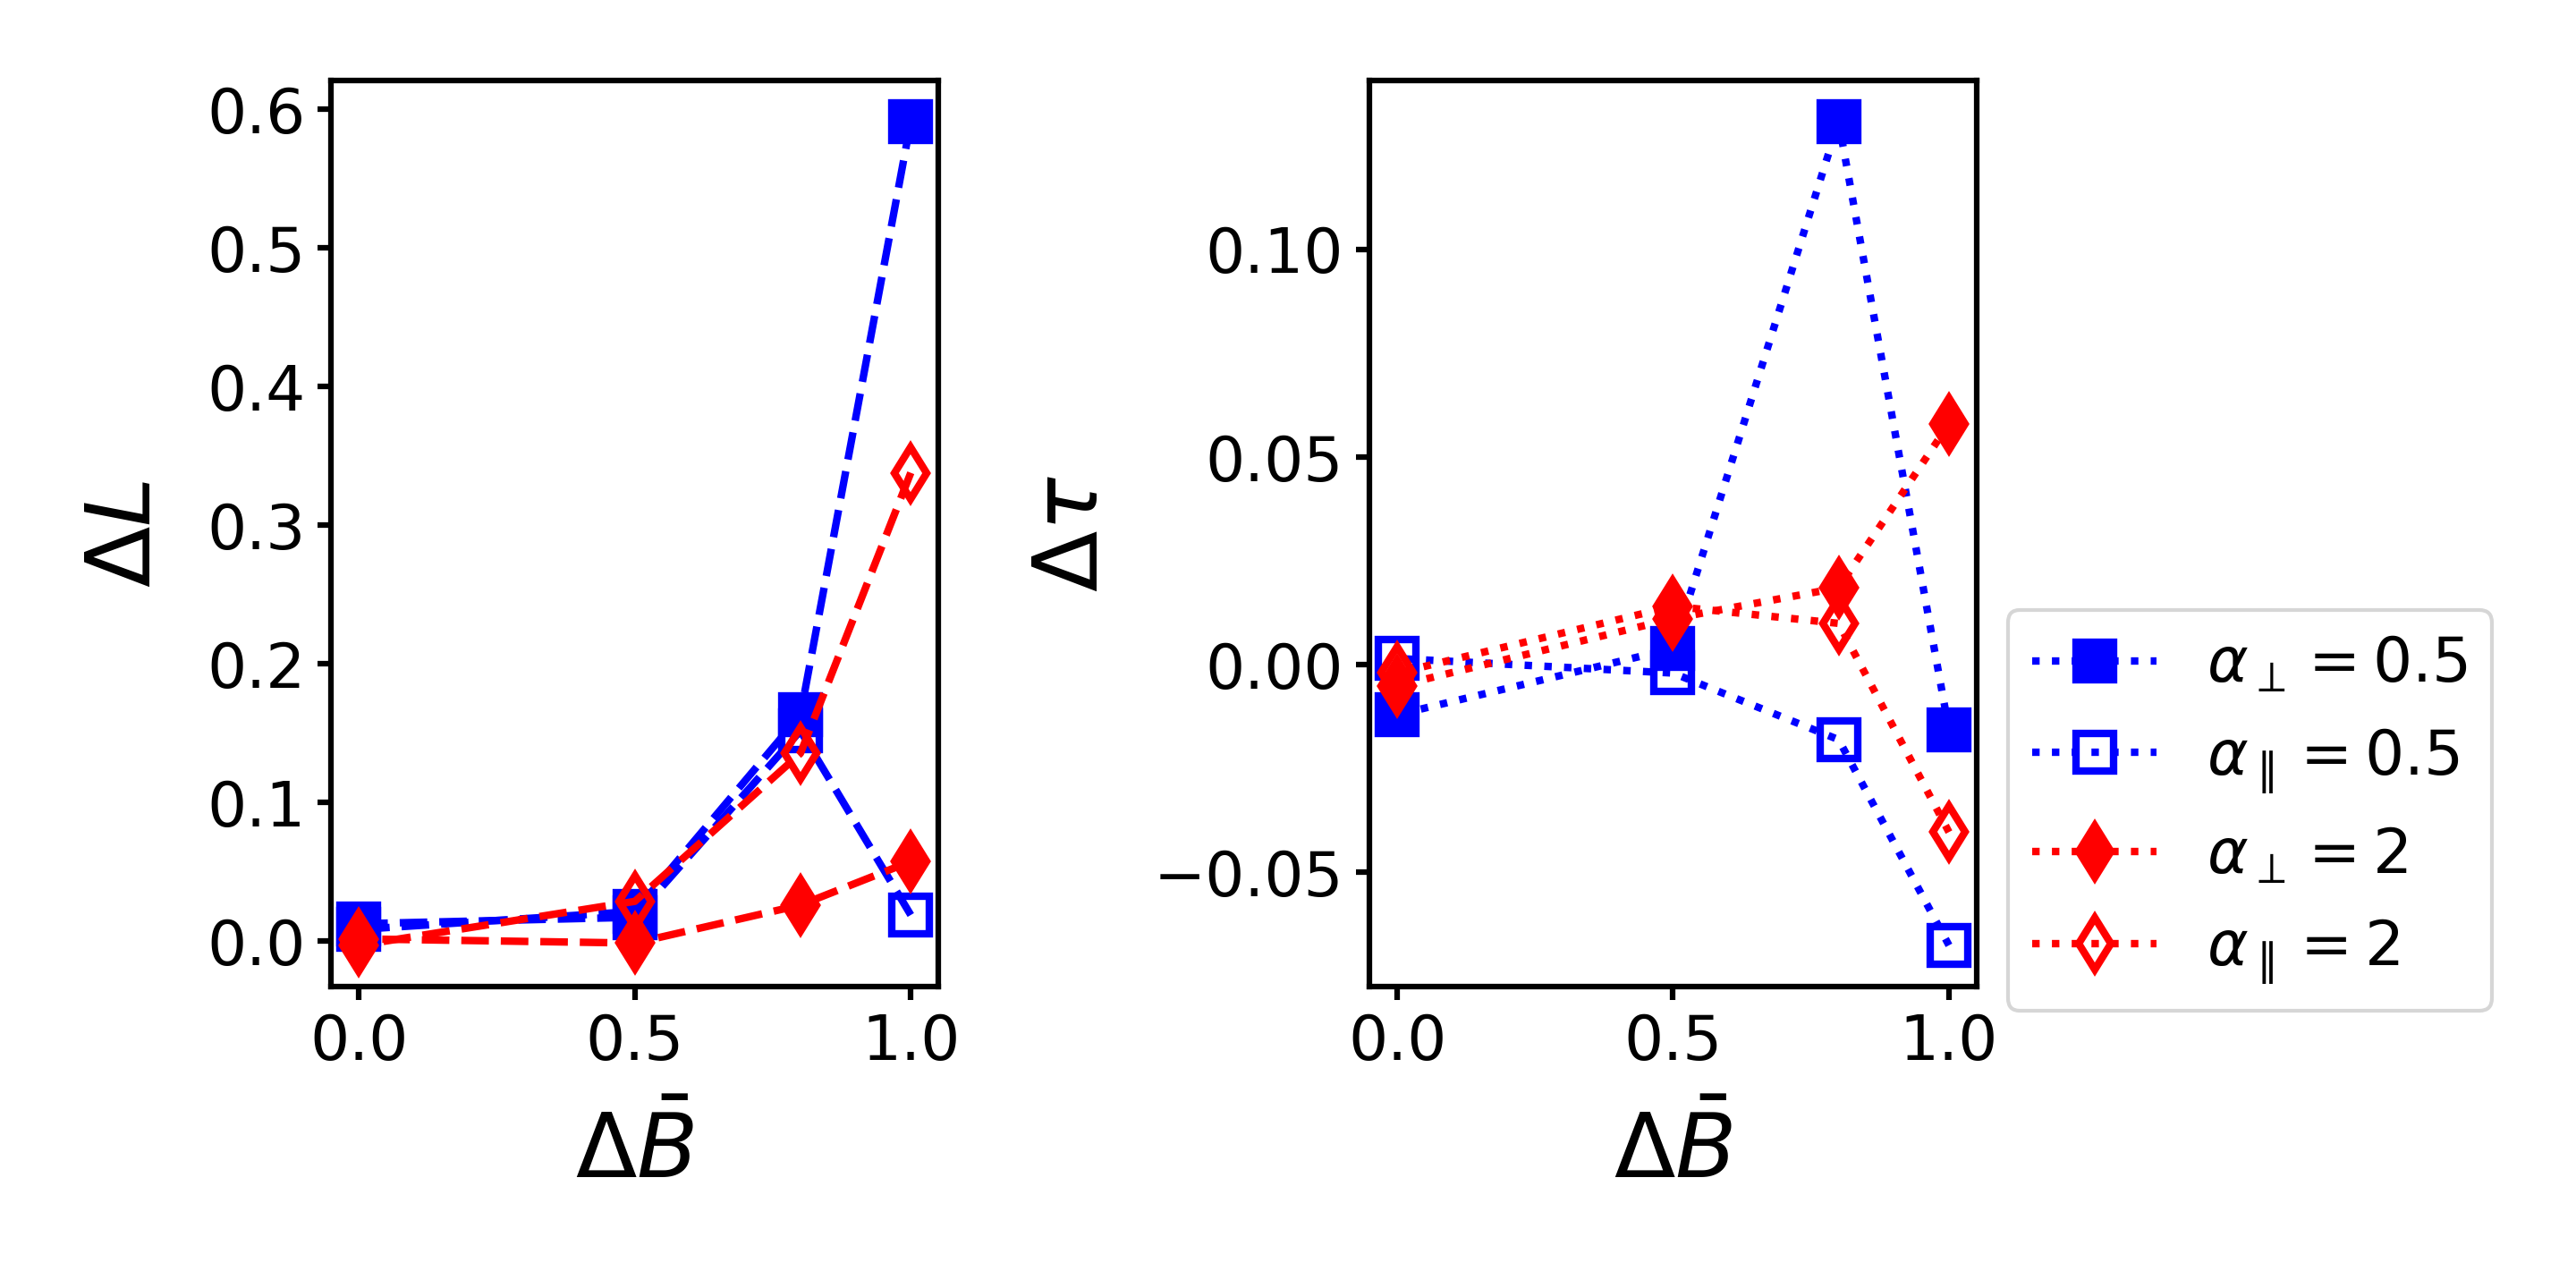
\includegraphics[scale = 0.5]{../figures/results/paper2/domain_size_aniso-field_up.png} 
\caption{Plotting the anisotropic domain sizes and tortuosity at the final timestep on the left and right respectively for bijels stabilized with 
         oblate and prolate ellipsoidal particles starting at different particle orders. We plot these results against the change in the applied field 
         strength, $\Delta B$. The anisotropic domain size is inversely correlated to the tortuosity and $L_{perp}$ changes for 
         a bijel made with $\bar{B} = 1 \rightarrow 1$ and $\bar{B}: 0 \rightarrow 1$ differ, suggesting that the processing history of the bijel is important.} 
\label{fig:domain_size_aniso-field_up} 
\end{figure}

From Figure \ref{fig:domain_size_aniso-field_up}, domain
size anisotropy is observed upon increasing the applied field
for both particle morphologies. Some domain anisotropy with no applied field can be observed, 
which increases upon application of the magnetic field. The directional domain sizes,
$L_{\perp}$ and $L_{\parallel}$ increase by $73\%$ and $7\%$
respectively for oblate particles and $10\%$ and $44\%$ respectively
for prolate particles. The axes that coarsens the most is consistent
with past work, explained through the directions particles reorient in
response to the applied magnetic field. The
tortuosity of the bijel is initially around $\tau \approx 1.5$,
consistent with simulations of the diffusive tortuosities of gyroid
structures using Lattice Boltzmann simulations.
\cite{luo_macroscopic_2020} Upon application of the field,
$\tau_{\perp}$ slightly decreases while $\tau_{\parallel}$
increases. Consistent with past work, an increase in the domain size sees a decrease in
tortuosity in that direction. \cite{karthikeyan_formation_2024}. The results show that the
tortuosity of the bijel is noticeably affected by the application of
magnetic fields.

As particles unjam and rejam at the interface due to reorientating to
the magnetic field, they adopt direction specific surface coverages
which manifest as anistropic domains upon jamming. The direction of the
anisotropy is different as the oblate particles have an axis of symmetry
in the short axis of the radius, while for the prolate particles it is
on the long axis. Thus during reorientation, the long axis of the oblate
particles will be orthogonal to the applied field and parallel for the
prolate particles. To characterize how the particle order changes on the
interface as a function of the magnetic field strength, we visualize the
particle monolayer of bijels stabilized by prolate particles in Figure
\ref{fig:particle_viz-field_up}.

\begin{figure} 
\centering 
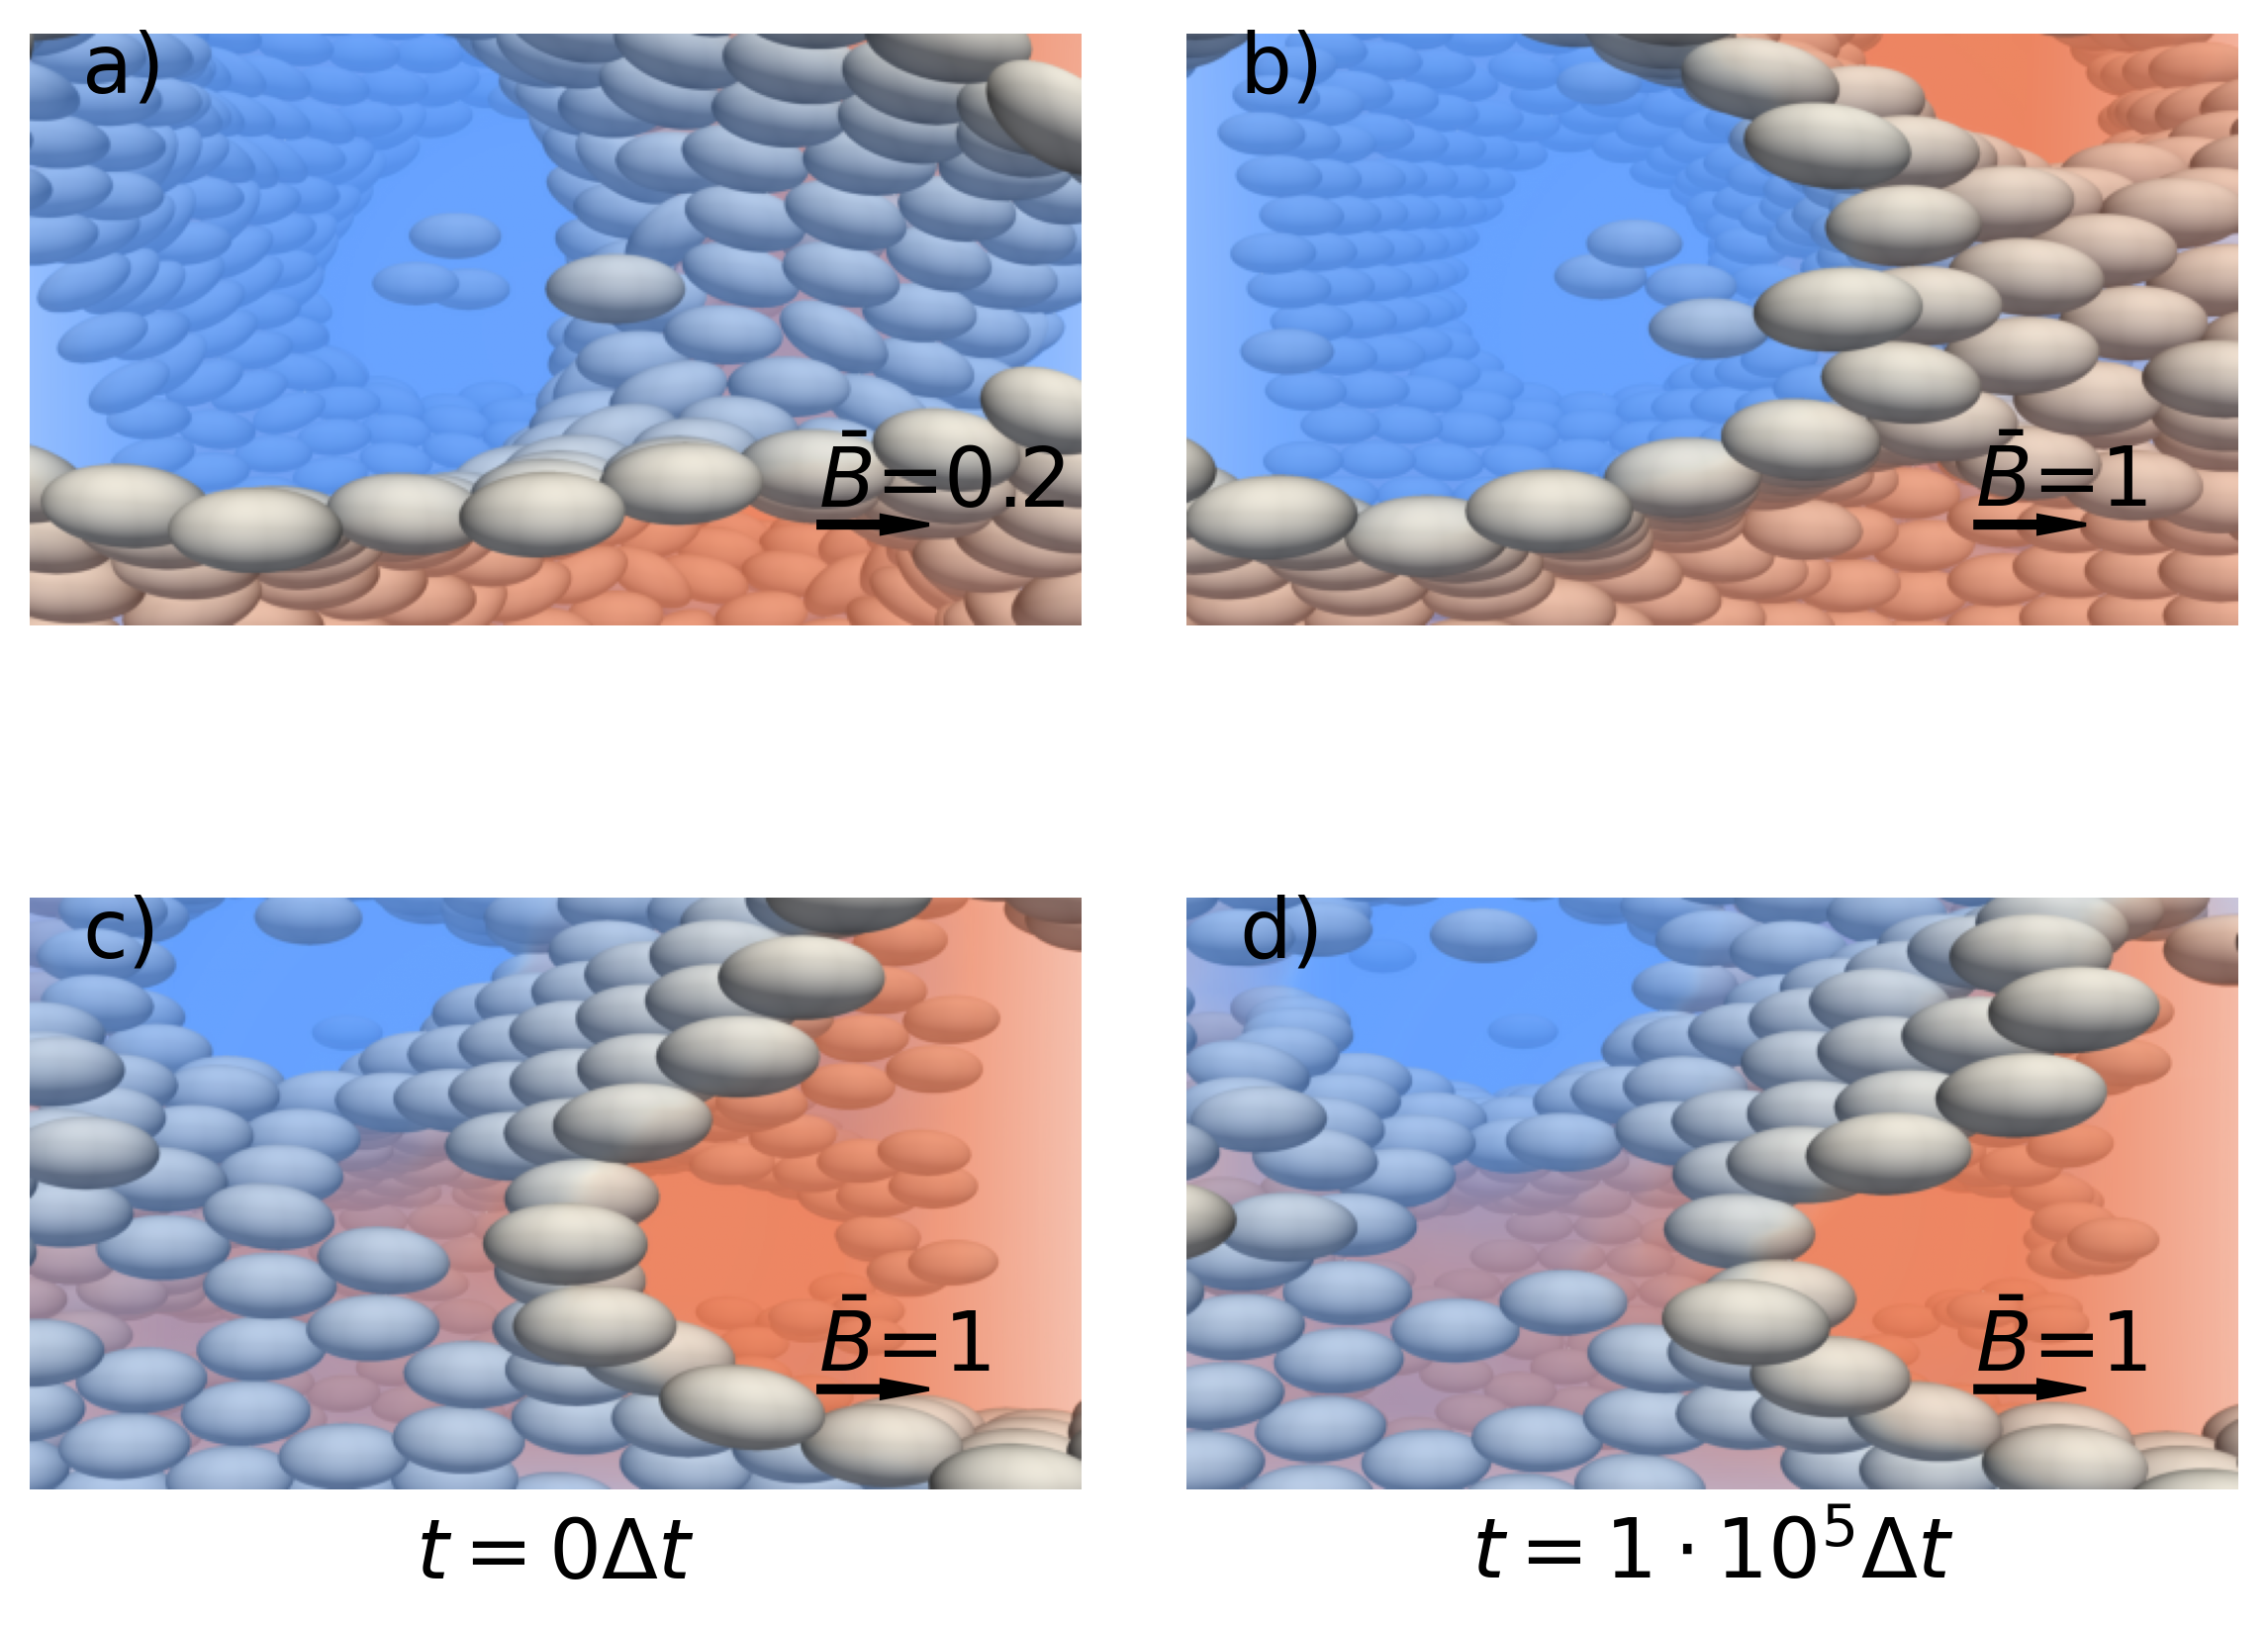
\includegraphics[scale=0.2]{../figures/results/paper2/particle_viz-field_up.png} 
\caption{Visualizations of bijels stabilized with oblate and prolate particles simulated at $t = 0$ (left column) and $t = 10^5$ (right column). 
         The first and third rows show the particle monolayer of bijels stabilized with oblate and prolate ellipsoids respectively with an applied 
         field of $\bar{B}_z = 0.2$. The second and fourth rows show the particle monolayer of bijels stabilized with oblate and prolate ellipsoids 
         respectively with an applied field of $\bar{B}_z = 1$. We increase the applied field to $\bar{B}_z = 1$ in both cases and show that particle 
         reorientation to the field occurs at the $\bar{B}_z = 0.2$ but not in the $\bar{B}_z = 1$ case.} 
\label{fig:particle_viz-field_up} 
\end{figure}

In Figure \ref{fig:particle_viz-field_up}, we see the effect of the
application of the magnetic field on the monolayer. The initial
configuration of particles at the monolayer show that even at initial
configuration of run $\bar{B}: 0.2 \rightarrow 1$, most particles are
oriented towards the field. Upon increasing the field strength to
$\bar{B} = 1$, all particles shown can be seen to be ordered to the
field, matching the results for the nematic order parameter shown in
Figure \ref{fig:domain_size-field_up}. We also observe the alignment of
the long axis of the particles to the magnetic field, demonstrating the
origin of the microstructure anisotropy. To understand how the particle
reorientation at the interface causes microstructure reorientation we
quantify the average interface angle, $\langle \psi \rangle$ and the
local interface order of the material, $\langle Q6 \rangle$ in Figure
\ref{fig:interface_angle-nint-field_up}.

Figure \ref{fig:interface_angle-nint-field_up} shows that
prolate and oblate particles respond differently at the interface upon application of a magnetic field
even with pre-existing ordering of the particles. We
show that there are three time evolution trends for
$\langle \psi \rangle$ and $\langle Q6 \rangle$ for both oblate and
prolate particles despite the differences in the initial state of the
particles. In oblate particles $\langle \psi \rangle$ begins closer to
$20 ^{\circ}$ as the axis of symmetry lies close to the interface
normal. For bijels experiencing a field strength history of
$\bar{B}: 0 \rightarrow 1$ and $\bar{B}: 0.2 \rightarrow 1$,
$\langle \psi \rangle$ increases, plateaus and increases again before
plateauing again. This is indicative of particles tilting at the
interface, before interfacial capillary interactions ``pause'' particle
reorientation before the applied magnetic field begins to cause
particles to tilt out of the interface. We see similar trends for bijels
stabilized by prolate particles. $\langle \psi \rangle$ begins near
$11 ^{\circ}$ and decrease before reorientation ceases before
$\langle \psi \rangle$ increases again.

When looking at $\langle Q6 \rangle$ for $\bar{B}: 0 \rightarrow 1$
and $\bar{B}: 0.2 \rightarrow 1$ for oblate particles, we see that the
trends are similar with an initial decrease, followed by a plateau and
increase over time before plateauing again. $\langle Q6 \rangle$
generally decreases with a large decrease observed for
\(\bar{B}: 0 \rightarrow 1\) from an initial hexagonally packed system
to a structure that is locally ordered but not close packed. $\langle Q6 \rangle$ increases before plateauing 
in both systems around 5000 timesteps. The significance of
this time is unknown for $\bar{B}: 0.2 \rightarrow 1$ but for
$\bar{B}: 1 \rightarrow 1$, this is approximately the local
crystallization point when $\langle Q6 \rangle \geq 0.38$.

For oblate particles, structural response dynamics
arise from particle tilting on the interface identified as the large
difference between the initial and final $\langle \psi \rangle$ with
an associated decrease in the interface coverage, initiating domain
coarsening. Interfacial tilting causes a loss in the
close packing of oblate particles at the interface. For prolate
particles, a small degree of particle tilting can be seen
from $\langle \psi \rangle$, although an increase in $\langle Q6 \rangle$ is observed
decreasing the interfacial area. Larger domain size response is
observed for the oblate particles as the interfacial area change from
particle tilting at the interface is larger than that of particles close
packing at the interface.

\begin{figure} 
    \centering 
    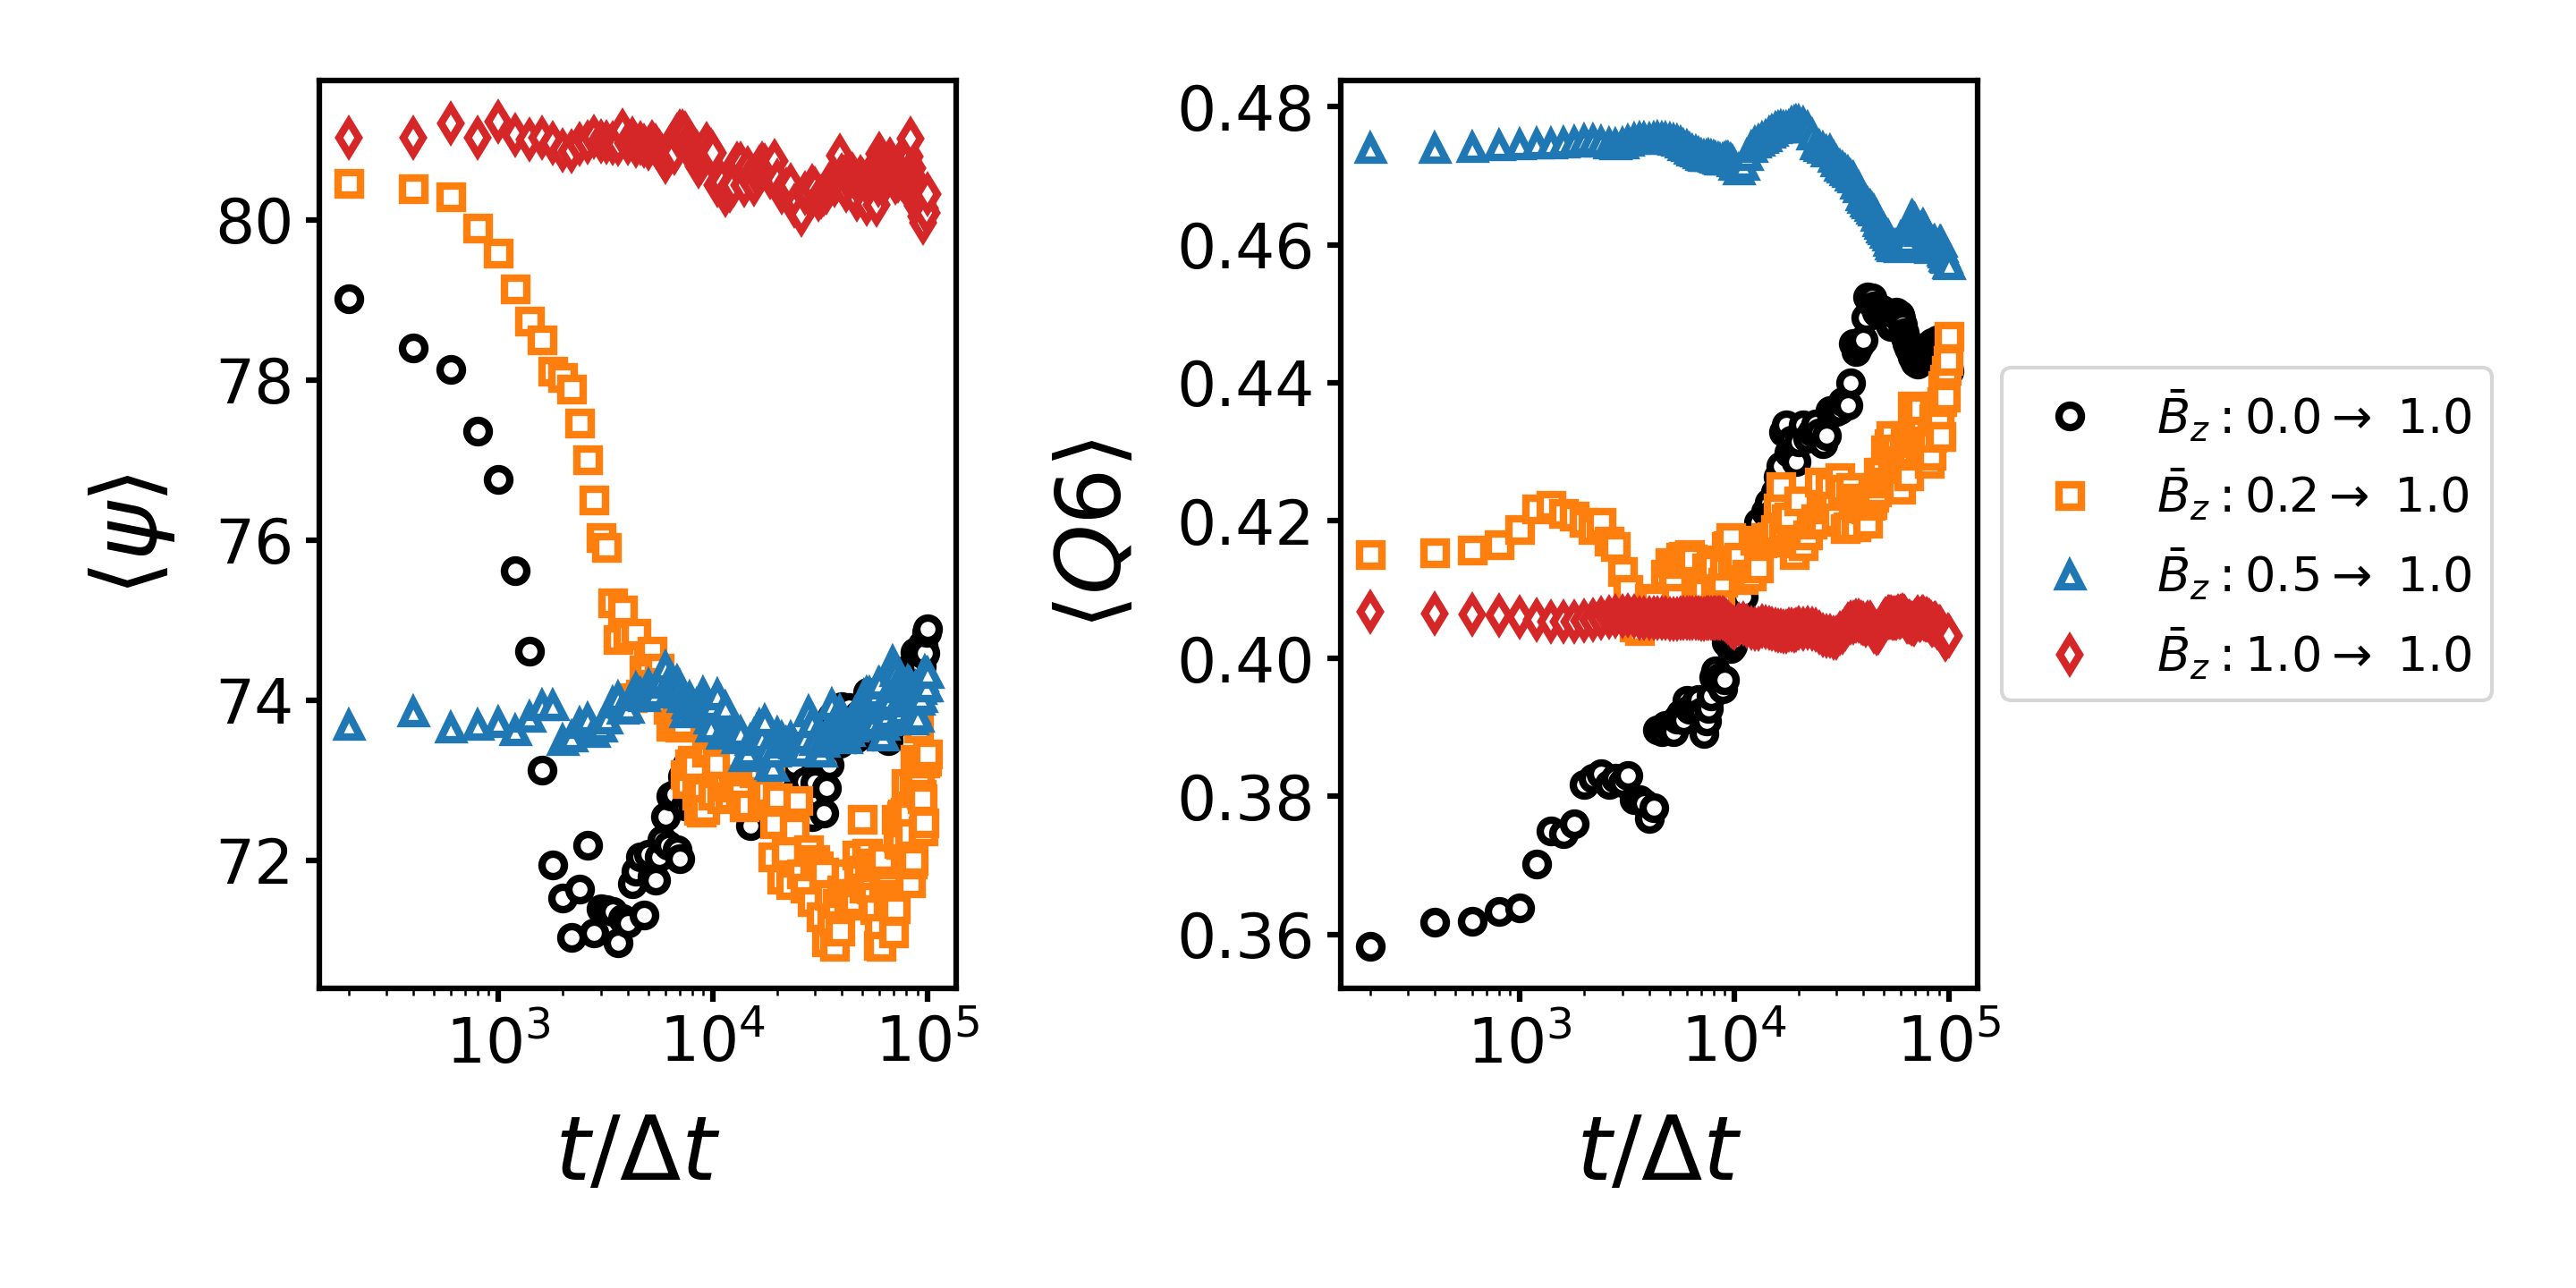
\includegraphics[scale=0.4]{../figures/results/paper2/interface_angle-nint-field_up.png} 
    \caption{Plots of the average interfacial angle $\psi$ and the number of particles on the interface $n_{int}$ on the left and right respectively, 
             plotted against time for bijels stabilized with ellipsoidal particles with aspect ratio 2. When looking at $\psi$, a change in dynamics can be 
             seen as the initial particle order increases. When looking at $n_{int}$, different dynamics are seen above and below the isotropic to nematic transition point. 
             Both results suggest that the ordering of particles is linked to the dynamics of domain coarsening.} 
    \label{fig:interface_angle-nint-field_up} 
\end{figure}

For both particle morphologies we analyze the response of bijels with a
field history of $\bar{B}: 0.5 \rightarrow 1$ and
$\bar{B}: 1 \rightarrow 1$.
$\langle Q6 \rangle$ decreases for bijels stabilized with oblate particles with
field application of $\bar{B}: 0.5 \rightarrow 1$ compared to an
increase for $\bar{B}: 1 \rightarrow 1$. This behavior arises from the
slight increase in the nematic order for particles in bijels
experiencing the $\bar{B}: 0.5 \rightarrow 1$ field application
history. The $\langle \psi \rangle$ results indicate that the
particles rearrange over time to lie flatter on the interface. For
bijels stabilized with prolate particles, We characterize a difference
in behavior between $\bar{B}: 0.5 \rightarrow 1$ and
$\bar{B}: 1 \rightarrow 1$. For the $\bar{B}: 0.5 \rightarrow 1$
case, a slight increase in $\langle \psi \rangle$ before a
decrease and increase is seen compared to the $\bar{B}: 1 \rightarrow 1$ case
where we characterize a slight decrease over time. We also characterize
a slight decrease in $\langle Q6 \rangle$ over time for the
$\bar{B}: 1 \rightarrow 1$ case while characterizing a larger decrease
for the $\bar{B}: 0.5 \rightarrow 1$ case. Similar to the oblate
particles, these results originate from the slight increase in the
nematic order for bijels experiencing the $\bar{B}: 0.5 \rightarrow 1$
field history.

\subsection{Decreasing the applied
field}\label{decreasing-the-applied-field}

Bijels are kinetically stable structures whose properties are dependent
upon the stability of the particle monolayer. Past work into responsive
emulsions have demonstrated resilience to microstructure changes after
application and removal of stimuli even after several months. \cite{cui_stabilizing_2013} However,
in the systems simulated above the particles need not necessarily be in
thermodynamically stable states when jammed upon removal of stimuli as
the particles take up a arrangements not observed when no field is
applied. In this section, we explore how removal of the magnetic field
changes the microstructure of the bijel as a function of the initial
particle order. We use bijels simulated under
$\bar{B}_{template} = 0, 0.2, 0.5, 1$ during formation of the bijel. Once
the microstructure has stabilized, we switch off the magnetic field and
observe the time evolution of the system for $t = 10^5$ timesteps.

\begin{figure} 
\centering 
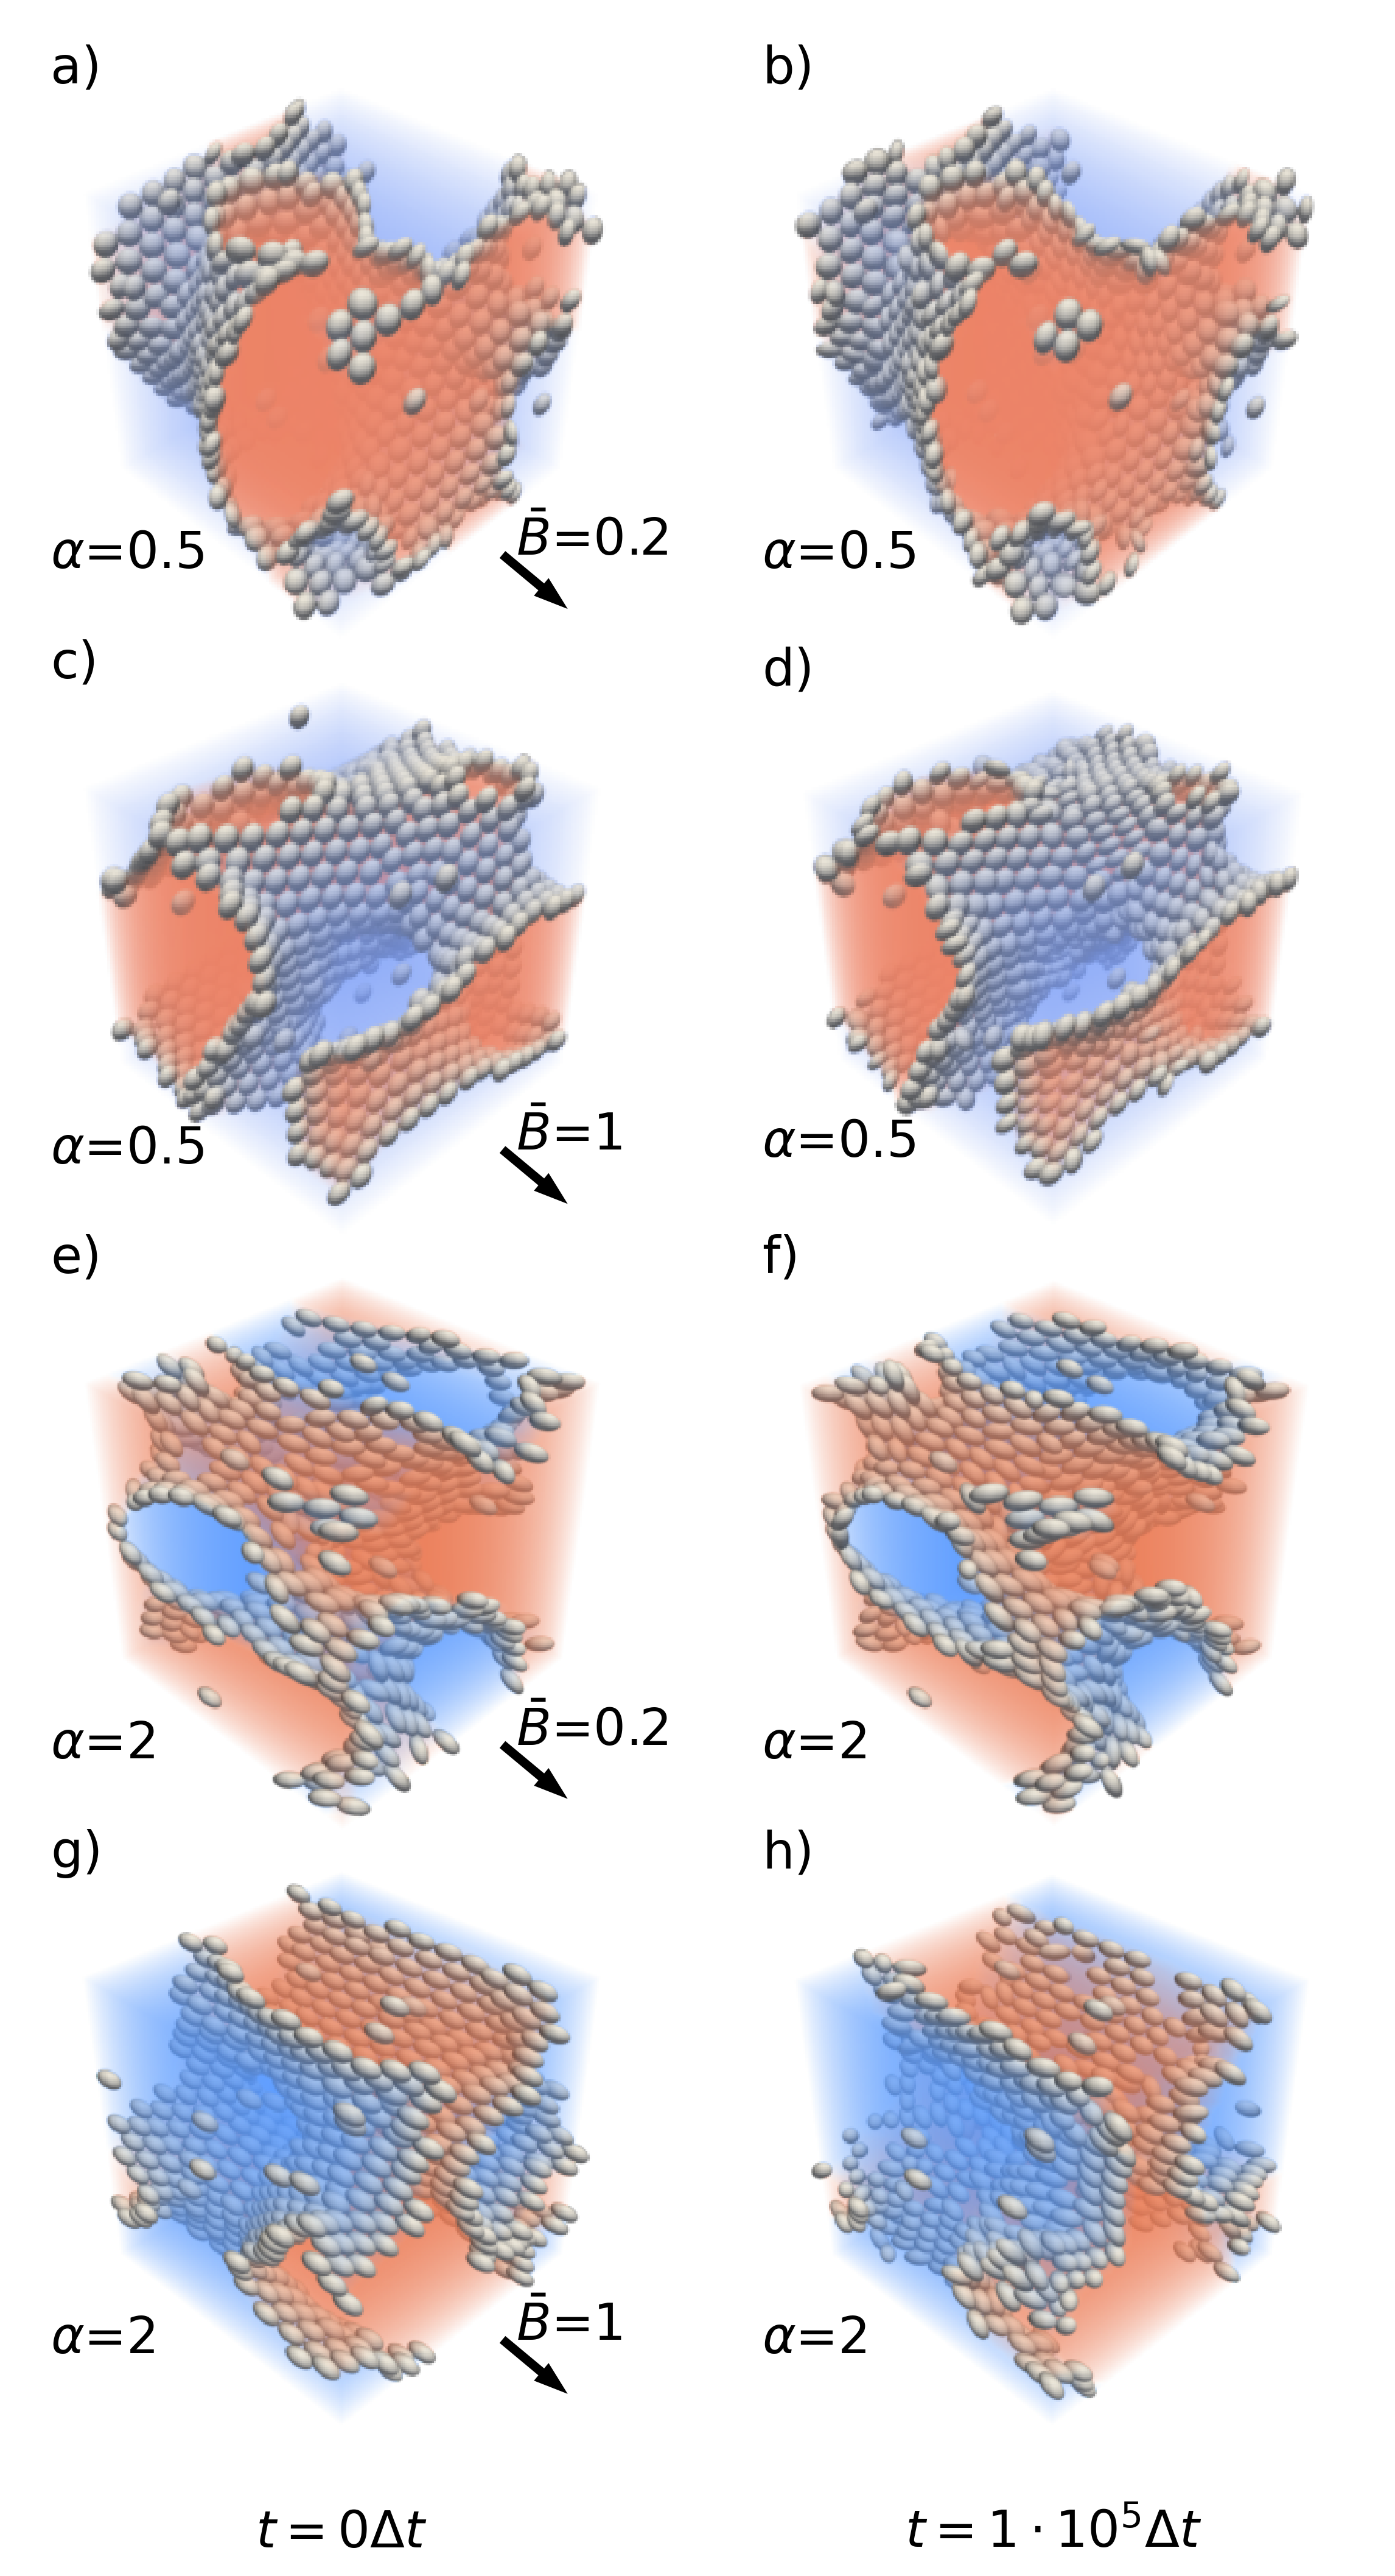
\includegraphics[scale=0.4]{../figures/results/paper2/microstructure_viz-field_down.png} 
\caption{Visualizations of bijels stabilized with oblate and prolate particles simulated at $t = 0$ (left column) and $t = 10^5$ (right column). 
         The first and third rows show the particle monolayer of bijels stabilized with oblate and prolate ellipsoids respectively with an applied 
         field of $\bar{B}_z = 0.2$. The second and fourth rows show the particle monolayer of bijels stabilized with oblate and prolate ellipsoids 
         respectively with an applied field of $\bar{B}_z = 1$. We switch off the applied field in both cases and show that while particle reorientation 
         occurs, it has little effect on the microstructure of the bijel.}
\label{fig:microstructure_viz-field_down}
\end{figure}

In Figure \ref{fig:microstructure_viz-field_down}, we visualize the time
evolution of the microstructure of bijels with processing history
$\bar{B}:0.2 \rightarrow 0$ (top) and $\bar{B}:1 \rightarrow 0$
(bottom). When switching the field off, the microstructure
remains largely the same, demonstrating the kinetic stability of bijels.
However, the particle monolayer, while still showing order, appears to
be slowly losing that order as particles are beginning to become
randomly oriented. This is especially obvious in the
$\bar{B}:1 \rightarrow 0$ process, demonstrating that the dynamics of
the system is dependent upon the initial order of the particle
monolayer.

\begin{figure} 
\centering 
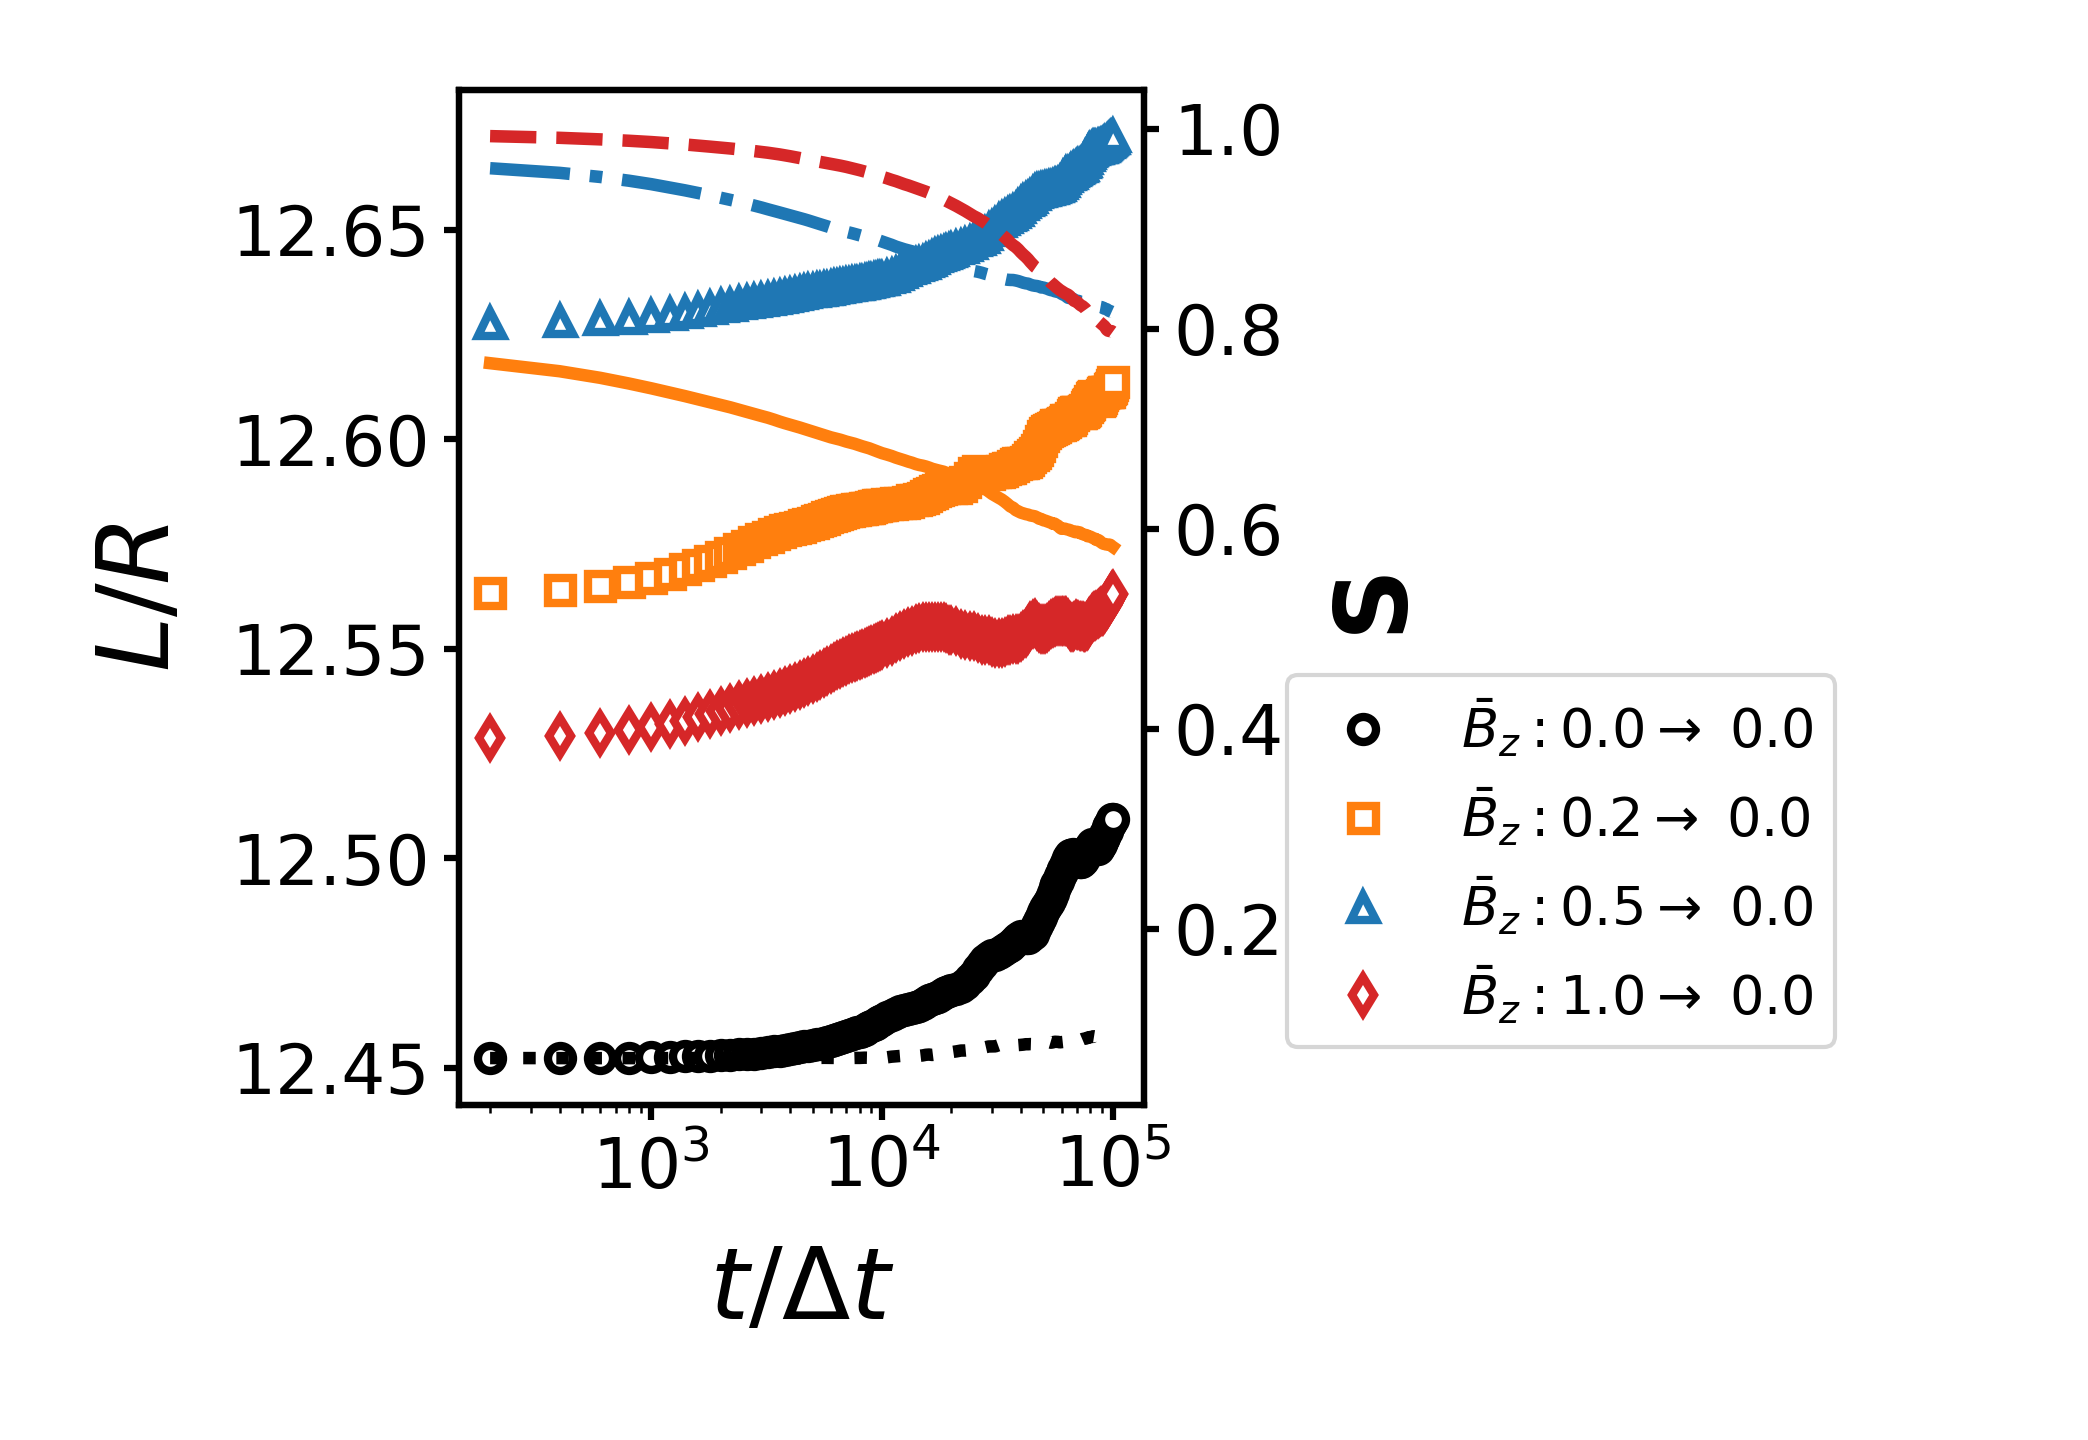
\includegraphics[scale=0.5]{../figures/results/paper2/domain_size-field_down.png} 
\caption{Plot of the spherically averaged domain size normalized with $R_p$ of the particle and the nematic order parameter of each bijel over time. 
         Each color represents bijel templates made with different field strengths $\bar{B}$. We show that there is domain coarsening when the field 
         is switched off, along with a reduction in the ordering of the particles.} 
\label{fig:domain_size-field_down} 
\end{figure}

The results in \ref{fig:domain_size-field_down}, show with the exception of $\bar{B}:0\rightarrow0$, all
domain sizes show a slow coarsening over time. This is reflected clearly
in the bijels stabilized by prolate particles, showing that that the
changes in properties of the particle monolayer due to the applied
magnetic field during bijel template simulation does not play a
significant role in the dynamics of the bijel. We attribute the large
increase in the domain size in oblate particle stabilized
$\bar{B}:0\rightarrow0$ case to be due to coalescence of two
domains, characterized as a two step process where slower long
timescale domain coarsening initially occurs followed by a rapid jump in the
domain size when coalscence between domains occur.

The nematic order parameter of all runs with prexisting particle order
show order dependent decreases, arising from interfacial forces causing
the particles to return to a thermodynamically optimum configuration on
the interface. To quantify is the coarsening that takes place is
anisotropic, We define the relative change in domain size as
$\Delta L = \frac{L_{f} - L_{i}}{L_{i}}$, where $L$ represents
either $L_{\perp}$ or $L_{\parallel}$. The same formulation is
applied to the tortuosity in the respective directional components. We
do this to characterize the $\Delta \bar{B}$ dependent changes
observed in the domain anisotropy. The results are presented in Figure
\ref{fig:domain_size_aniso-field_up}.

\begin{figure} 
\centering 
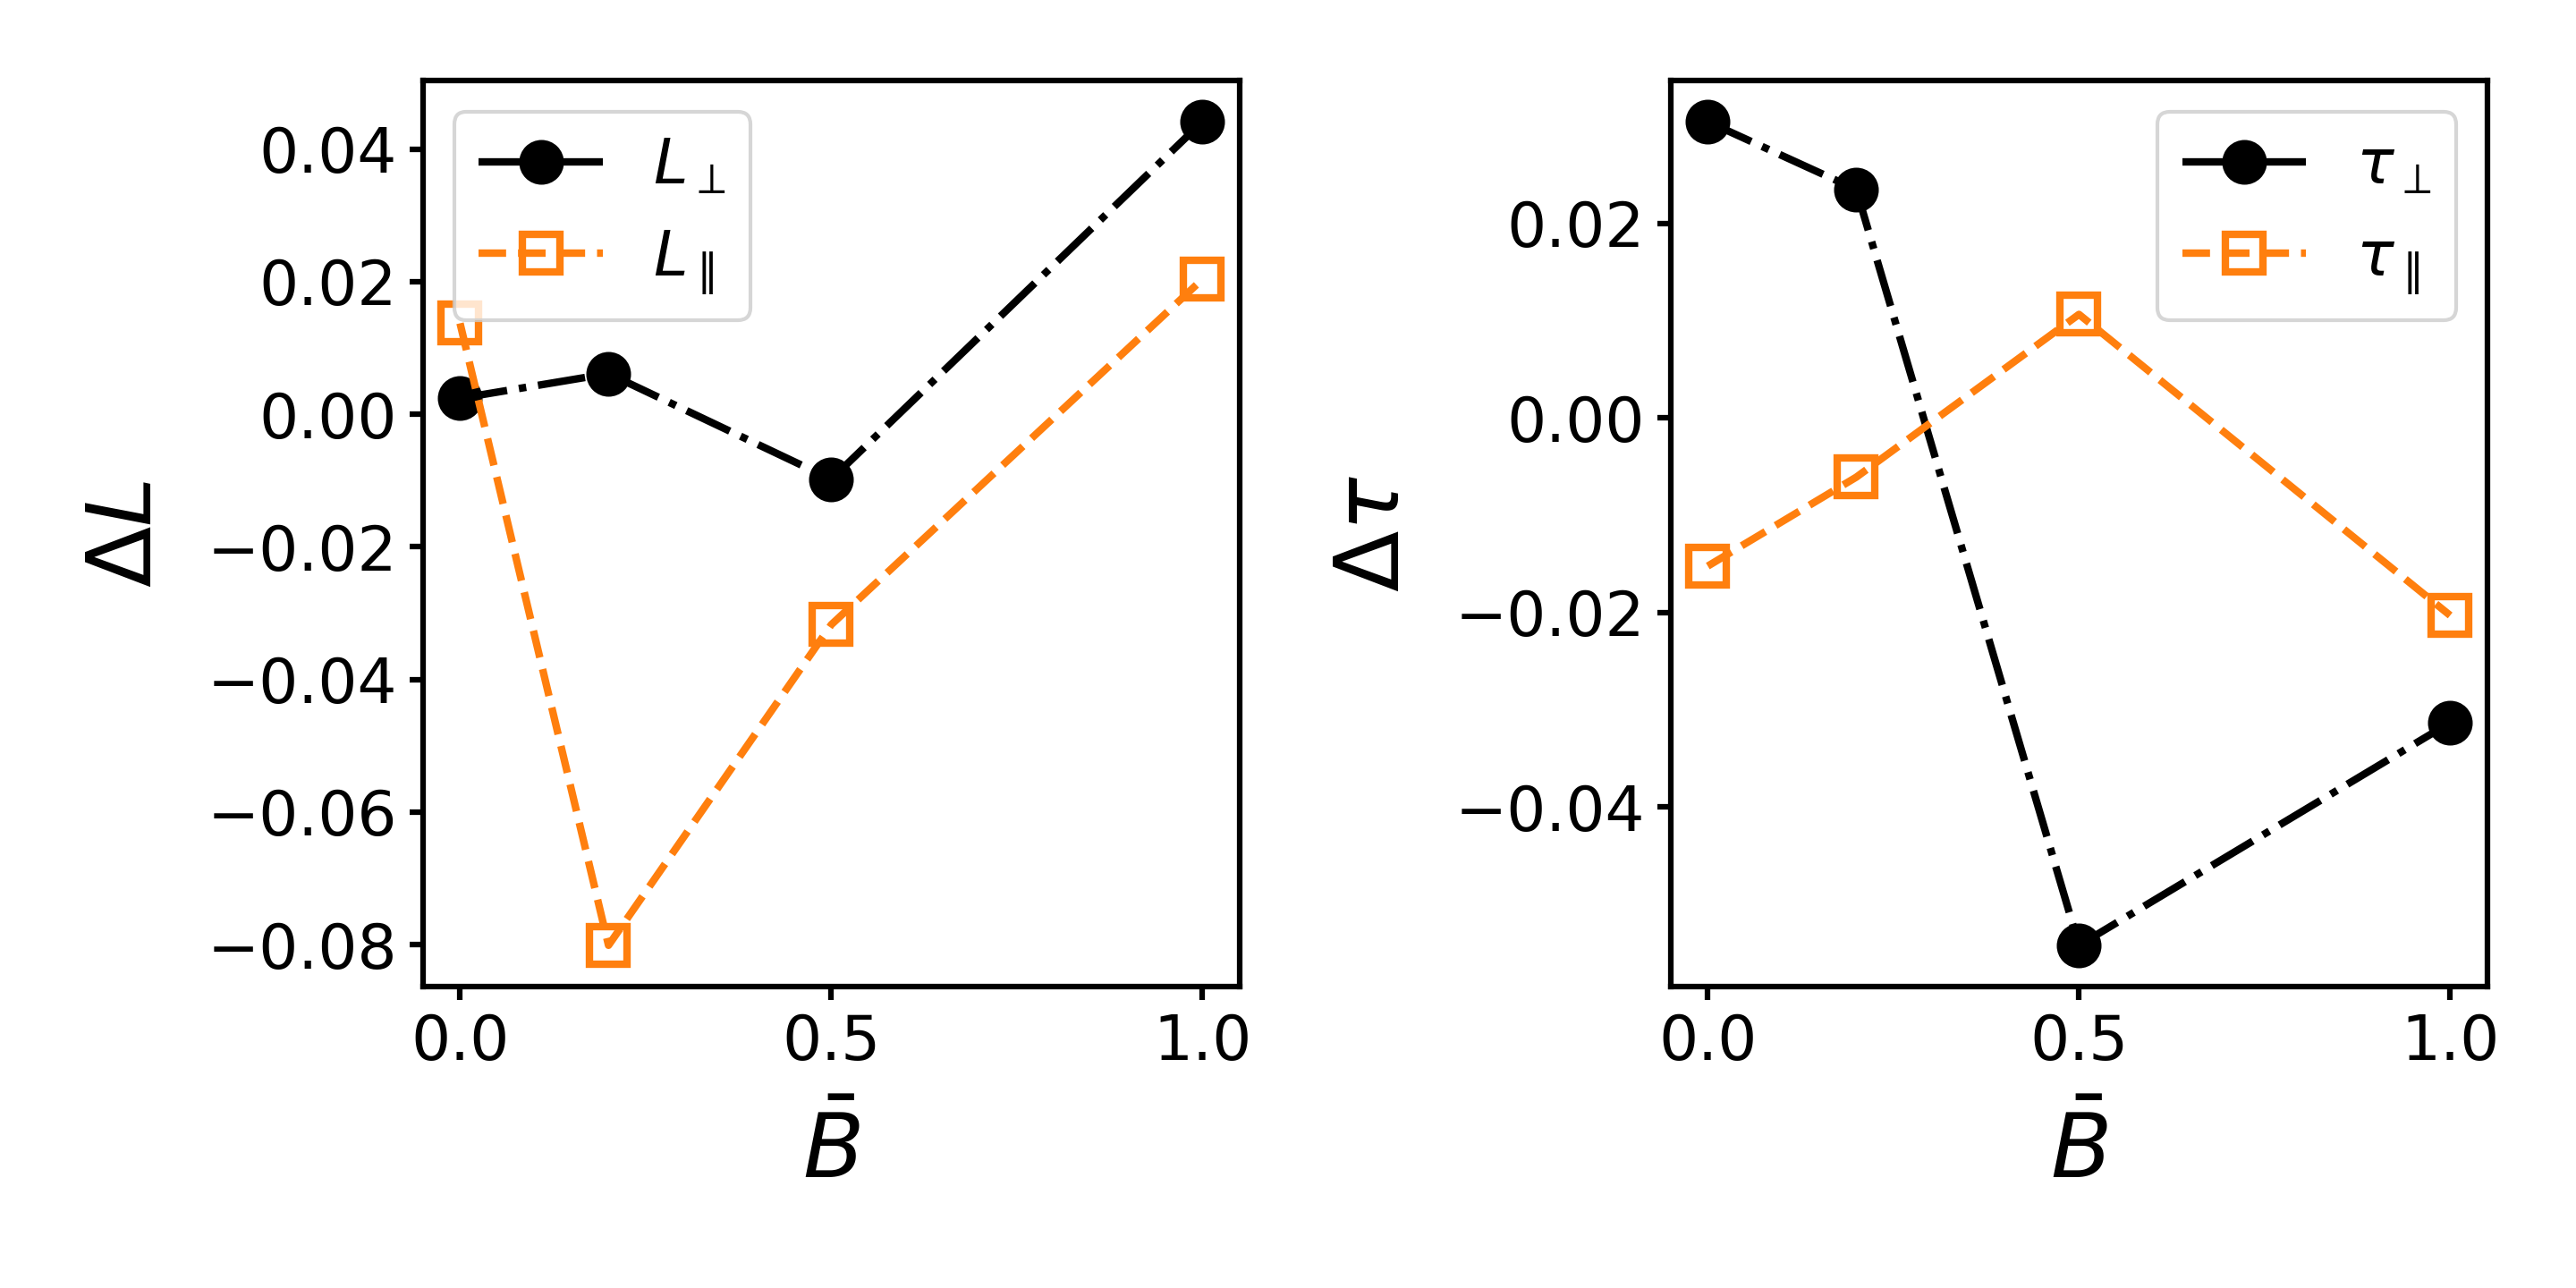
\includegraphics[scale = 0.5]{../figures/results/paper2/domain_size_aniso-field_down.png} 
\caption{Plotting the anisotropic domain sizes and tortuosity at the final timestep on the left and right respectively for bijels stabilized with oblate and 
         prolate ellipsoidal particles starting at different particle orders. We plot these results against the change in the applied field strength, 
         $\Delta B$ and show that there are only minor differences in the microstructure of stimuli responsive bijels once the magnetic field is switched off.} 
\label{fig:domain_size_aniso-field_down} 
\end{figure}

Figure \ref{fig:domain_size_aniso-field_down}, shows that there are
small $\Delta \bar{B}$ dependent changes in the anisotropic domain
size and tortuosity for both particle morphologies. However, there are
no clear trends that can be developed from these plots, suggesting that
the changes are overall isotropic and any differences observed arise
from the arrangement of particles. This suggests that the response of
the material to the removal of a magnetic field is isotropic and only
dependent upon the capillary interactions with the particle monolayer.
We showed earlier that the application of magnetic fields change the
local state of the particles at the interface. However the results shown
thus far demonstrate that that these changes do not seem to affect the
coarsening of the bijel once stimuli is removed. To investigate why this
is the case, we plot $\langle \psi \rangle$ and
$\langle Q6 \rangle$ for bijels stabilized with ellipsoidal particles
below.

\begin{figure} 
\centering 
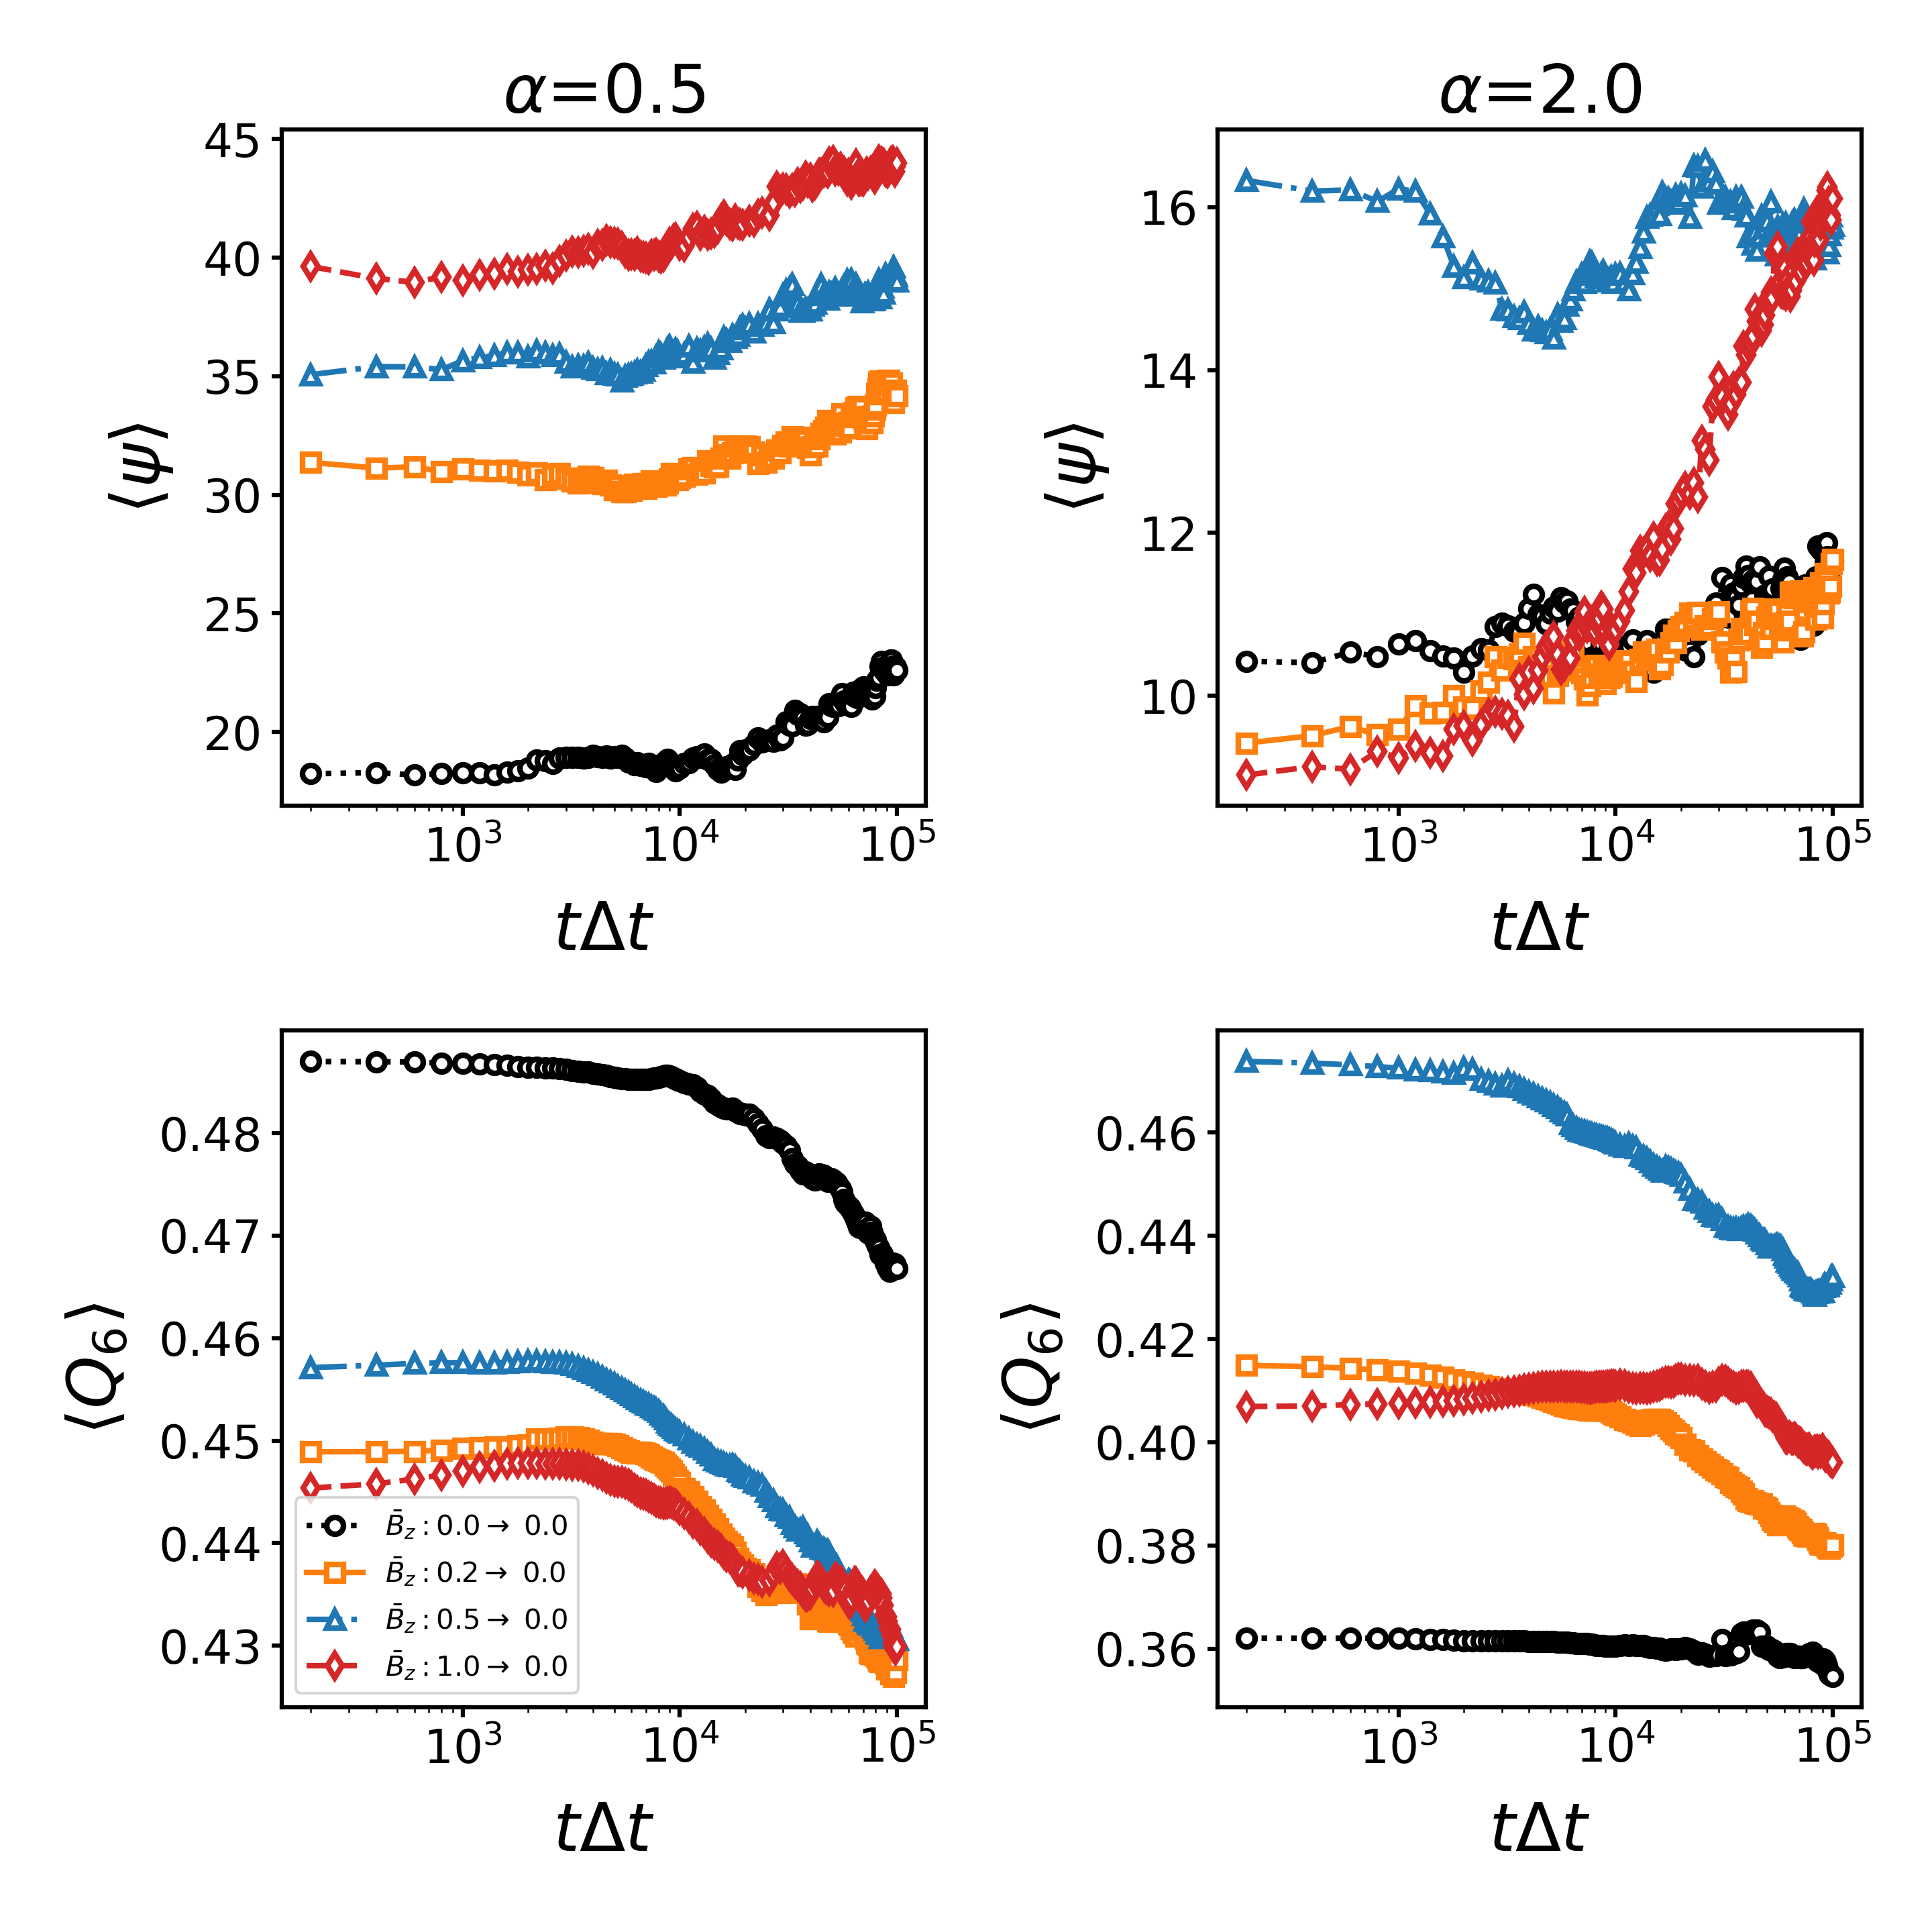
\includegraphics[scale=0.4]{../figures/results/paper2/interface_angle-nint-field_down.png} 
\caption{Plots of the average interfacial angle $\psi$ and the number of particles on the interface $n_{int}$ on the left and right respectively, 
         plotted against time for bijels stabilized with ellipsoidal particles with aspect ratio 2. When looking at $\psi$, the $\bar{B}:1 \rightarrow 1$ 
         case looks distinctly different from the other processes. At $\bar{B} = 1$, the particles are totally ordered to the field. This suggests that 
         the presence of some particle disorder resists domain coarsening.} 
\label{fig:interface_angle-field_down} 
\end{figure}

From Figure \ref{fig:interface_angle-field_down}, there are minor differences to the time when $\langle \psi \rangle$ and $\langle Q6 \rangle$
begin to change. We also characerize that $\langle \psi \rangle$ increases for both particle morphologies, even for systems that have initial ordering.
Similarly, $\langle Q6 \rangle$ decreases for all systems. Thus, the presence of ordering does not greatly affect trends in the evolution of the
particle monolayer, and thus has an insignificant effect on the microstructure of the bijel.

From the microstructure evolution, steric effects are the
driving force behind microstructure changes in the absence of a magnetic
field. Even though we observe that the interface angle and Steinhardt
order parameter show substantial changes from the scenario where no
field is applied, these are insufficient to change the average steric
effect driven particle monolayer rearrangement observed, causing
coarsening of the bijel at long timescales to possess trends similar to what was observed by
Gunther et al. \cite{gunther_timescales_2014}

\section{Conclusions}

Owing to the applicability of bijels in the catalyst support, filtration membrane and drug release spaces, we were interested in identifying how bijels stabilized 
by magnetically responsive ellipsoidal particles could be used to create active soft matter. In this work, we have studied the effect of the application, increase 
or removal of magnetic fields on the structural response of bijels stabilized by magnetically responsive ellipsoids using hybrid Lattice Boltzmann-Molecular Dynamics 
simulations. We first characterized the hysteresis curve of the bijel, identifying that the process history dependence of the bijel microstructure. To identify why 
We observed the path dependence and the microstructure change observed when applying magnetic fields after synthesis, we considered three starting setups; The first 
applying a field of varying strength to bijel templates that were simulated with no magnetic field applied. The second involved increasing the applied field 
strength onto bijel templates that were simulated with increasing field strengths. The final setup involves removing a field from bijel templates that were simulated 
with various field strengths. 

We found that application of magnetic fields onto bijels stabilized by magnetically responsive ellipsoidal particles results in an average microstructure change up to 
$5\%$ when investigating changes in the average microstructure. We also identified that the structures become anisotropic upon application of the magnetic field for 
oblate and prolate particles. The anisotropy is particle dependent with bijels stabilized by oblate particles seeing an increase in $L_{\perp}$ of up to $60\%$ and for 
prolate particles an increase in $L_{\parallel}$ of up to $40\%$ with a corresponding decrease in the tortuosity in that axis. This is caused by the reorientation of the 
particles to the magnetic field, followed by domain coarsening as the interfacial coverage of the particles decrease, before jamming in place again. We characterize that 
while particle reorientation to the applied field initiates microstructural response, local rearrangement of the particle monolayer is the controlling mechanism of 
domain size evolution as characterized by identifying the dominant timescales 
of response for both particle morphologies. However, their time evolution is different with bijels stabilized by prolate particles undergoing a local crystallization when 
the average six fold Steinhardt order parameter or $\langle Q_6 \rangle \geq 0.38$. For bijels stabilized by oblate particles, a global minimum of the $\langle Q_6 \rangle$ 
characterizes the dynamics of the system.

When increasing the applied field strength, we observe that the difference between the final and initial magnetic fields is correlated to the domain size change observed. 
We observe that the anisotropic domain size changes are also dependent upon this difference, with the largest difference being observed when characterizing a bijel template 
simulated under no field before having a field strength of $\bar{B} = 1$ applied to it. When looking at the particle monolayer, we characterize three behaviors seen from the 
average interfacial angle $\langle \psi \rangle$ and $\langle Q_6 \rangle$. These behaviors are further differentiated for each particle morphology. For oblate particles, 
the first behavior is characterized as a reorientation of the particle on the interface seen as an increase in $\langle \psi \rangle$ over time with a corresponding decrease 
in $\langle Q_6 \rangle$ as the particles do not close pack anymore. For prolate particles, we see a slight reduction in $\langle \psi \rangle$ and greater ordering of the 
particles from $\langle Q_6 \rangle$. The second behavior originates from small reorientations of the particles at the monolayer which do not greatly affect the interfacial 
angle but cause a loss or gain of particle order on the interface. The final behavior is characterized as long timescale domain coarsening as there is no change between the 
applied magnetic field and the magnetic field used to simulate the template.

Finally, when decreasing the magnetic field strength, we observe little difference between bijel templates made with any field strength and no field. From the average domain 
size, we see that the bijels coarsen at approximately the same rate. Upon further investigation of the microstructure anisotropy, we identify that the anisotropic structure 
does not change as well, suggesting coarsening effects are independent of the effect of the local differences at the particle monolayer. After characterizing 
$\langle \psi \rangle$ and $\langle Q_6 \rangle$, we see differences at the initial state which, while changing the initiation point of the dynamics, does not play a large
 role otherwise. Thus any domain size change observed when removing a field is due to interfacial capillary interactions. 

It has been shown how the domain size and tortuosity can be used to adjust the flow rate, separations efficiency or reaction rate in applications such as cross-flow reactors, 
drug delivery and liquid-liquid extraction. These results show that the properties of bijels can be tuned in-situ for these applications although it appears that it can only 
be done once. With the results presented here, we have considered only one set of parameters that control the dynamics. Parameters not changed such as the fluid density, 
viscosity, surface tension and volume fraction of particles may impact the mechanisms and rate of domain size control. We also do not consider magnetic 
fields applied in different directions which even in this simple setup may be able to modify the microstructure considerably, or gradient magnetic fields which may allow 
more effective unjamming and re-jamming dynamics for further microstructure modification than what has been shown here.

Effects such as the steric hindrance between particles may lessen as particle size reduces as particles are more easily able to conform to the curvature of the interface. 
The impact this may have on the results seen with the micron-sized particles used here is unknown. In many of the applications listed above, it is also unknown how changes 
in the spacing between particles affect underlying reactivity, selectivity or diffusion rates which have implications past the domain size and tortuosity changes characterized 
in the literature. Furthermore, it is unknown how additional particle interactions such as chemical cross-linking or charge affect the results seen here. Both strategies are 
used in bijels to reinforce them against shear to facilitate higher shear rates, useful in cross-flow reactors and separation membranes. In conclusion, our simulations provide 
qualitative trends into the expected microstructure change and their underlying mechanisms and timescales when applying or removing a field from a bijel stabilized by 
anisotropic particles by modifying their orientation and packing.